% $Author$
% $Date$
% $Revision$
%=================================================================
\ifx\wholebook\relax\else
% --------------------------------------------
% Lulu:
	\documentclass[a4paper,10pt,twoside]{book}
	\usepackage[
		papersize={6in,9in},
		hmargin={.75in,.75in},
		vmargin={.75in,1in},
		ignoreheadfoot
	]{geometry}
	% $Author$ Martial
% $Date$ Wed Oct 10 13:34:55 CEST 2007
% $Revision$ source: SBE 12715 
% Last Changed Date: 2007-10-08 21:32:45 +0200 (Mon, 08 Oct 2007)
%=============================================================
% NB: documentclass must be set in main document.
% Allows book to be generated in multiple formats.
%=============================================================
%:Packages
\usepackage[french]{babel}
\usepackage[T1]{fontenc}  %%%%%% really important to get the code directly in the text!
\usepackage{lmodern}
%\usepackage[scaled=0.85]{bookmanx} % needs another scale factor if used with \renewcommand{\sfdefault}{cmbr}
\usepackage{palatino}
\usepackage[scaled=0.85]{helvet}
\usepackage{microtype}
\usepackage{graphicx}
\usepackage{theorem}
\usepackage[utf8]{inputenc}
% ON: pdfsync breaks the use of p{width} for tabular columns!
\ifdefined\usepdfsync\usepackage{pdfsync}\fi % Requires texlive 2007
%=============================================================
%:More packages
%Stef should check which ones are used!
%\usepackage{picinpar}
%\usepackage{layout}
%\usepackage{color}
%\usepackage{enum}
%\usepackage{a4wide}
% \usepackage{fancyhdr}
\usepackage{ifthen}
\usepackage{float}
\usepackage{longtable}
\usepackage{makeidx}
\usepackage[nottoc]{tocbibind}
\usepackage{multicol}
\usepackage{booktabs}	% book-style tables
\usepackage{topcapt}	% enables \topcaption
\usepackage{multirow}
\usepackage{tabularx}
%\usepackage[bottom]{footmisc}
\usepackage{xspace}
\usepackage{alltt}
\usepackage{amssymb,textcomp}
\usepackage[usenames,dvipsnames]{color}
%\usepackage{colortbl}
\usepackage[hang]{subfigure}\makeatletter\def\p@subfigure{\thefigure\,}\makeatother
\usepackage{rotating}
\usepackage{enumitem}	% apb: allows more control over tags in enumerations
\usepackage{verbatim}     % for comment environment
\usepackage{varioref}	% for page references that work
\labelformat{footnote}{\thechapter--#1} % to distinguish citations from jurabib
\usepackage{needspace}
\usepackage{isodateo} % enable \isodate
\usepackage[newparttoc]{titlesec}
\usepackage{titletoc}
\usepackage{eurosym}
\usepackage{wrapfig}

\usepackage[
	super,
	citefull=first,
	authorformat={allreversed,and},
	titleformat={commasep,italic}
]{jurabib} % citations as footnotes
\usepackage[
	colorlinks=true,
	linkcolor=black,
	urlcolor=black,
	citecolor=black
]{hyperref}   % should come last

%=============================================================
%:URL style
\makeatletter

\def\url@leostyle{%
  \@ifundefined{selectfont}{\def\UrlFont{\sf}}{\def\UrlFont{\sffamily}}}
% ajouter par Martial pour \traduit (met une dague dans les \doublebox
\def\thempfootnote{\fnsymbol{mpfootnote}}

\makeatother
% Now actually use the newly defined style.
\urlstyle{leo}
%=============================================================
%:Booleans
\newboolean{lulu}
\setboolean{lulu}{false}
\newcommand{\ifluluelse}[2]{\ifthenelse{\boolean{lulu}}{#1}{#2}}
%=============================================================
%:Names
\newcommand{\SUnit}{SUnit\xspace}
\newcommand{\sunit}{SUnit\xspace}
\newcommand{\xUnit}{$x$Unit\xspace}
\newcommand{\JUnit}{JUnit\xspace}
%\newcommand{\XP}{eXtreme Programming\xspace}
\newcommand{\st}{Smalltalk\xspace}
\newcommand{\Squeak}{Squeak\xspace}
\newcommand{\sq}{Squeak\xspace}
\newcommand{\sqmap}{SqueakMap\xspace}
\newcommand{\squeak}{Squeak\xspace}
%\newcommand{\sbe}{\url{scg.unibe.ch/SBE}\xspace}
%\newcommand{\sbe}{\url{squeakbyexample.org}\xspace}
\newcommand{\sbe}{\url{SqueakByExample.org}\xspace}
% squeak-fr: adresse de la version francaise
\newcommand{\spe}{\url{SqueakByExample.org}\xspace} % ?/FR
\newcommand{\sba}{\url{SquareBracketAssociates.org}\xspace}

% squeak-fr: ajout de la \squeakdev pour eviter les problemes de
% changements d'url rencontres dans la VO:
\newcommand{\squeakdev}{\url{www.squeaksource.com/ImageForDevelopers}\xspace} %ou
%\newcommand{\squeakdev}{\url{squeak.ofset.org/squeak-dev}\xspace}

%=============================================================
%:Editorial comment macros
\newcommand{\nnbb}[2]{
    \fbox{\bfseries\sffamily\scriptsize#1}
    {\sf\small$\blacktriangleright$\textit{#2}$\blacktriangleleft$}
   }
\newcommand{\ab}[1]{\nnbb{Andrew}{#1}}
\newcommand{\sd}[1]{\nnbb{St\'{e}f}{#1}}
\newcommand{\md}[1]{\nnbb{Marcus}{#1}}
\newcommand{\on}[1]{\nnbb{Oscar}{#1}}
\newcommand{\damien}[1]{\nnbb{Damien}{#1}}
\newcommand{\lr}[1]{\nnbb{Lukas}{#1}}
\newcommand{\orla}[1]{\nnbb{Orla}{#1}}
%\newcommand{\here}{\nnbb{CONTINUE}{HERE}}
\newcommand{\here}{\nnbb{CONTINUE}{ICI}}

%=============================================================
%:Abbreviation macros
\newcommand{\ie}{\emph{c-\`a-d.}\xspace}
\newcommand{\cad}{\emph{c-\`a-d.}\xspace}
%\newcommand{\eg}{\emph{e.g.},\xspace}
\newcommand{\eg}{\emph{par ex.},\xspace}
\newcommand{\parex}{\emph{par ex.},\xspace}
\newcommand{\etc}{etc\xspace}
%=============================================================
%:Cross reference macros

% [squeak-fr] martial: remarquez les articles devant les noms
\newcommand{\charef}[1]{le chapitre~\ref{cha:#1}\xspace}
% note de martial: utilise dans chapitre Syntax.tex: a redefinir
\newcommand{\charefs}[2]{les chapitres~\ref{cha:#1} et \ref{cha:#2}\xspace}
\newcommand{\secref}[1]{la section~\ref{sec:#1}\xspace}
\newcommand{\figref}[1]{la figure~\ref{fig:#1}\xspace}
\newcommand{\Figref}[1]{La figure~\ref{fig:#1}\xspace}
\newcommand{\appref}[1]{l'annexe~\ref{app:#1}\xspace}
\newcommand{\tabref}[1]{la table~\ref{tab:#1}\xspace}
% defini pour le chapitre Messages.tex
\newcommand{\Tabref}[1]{La table~\ref{tab:#1}\xspace}

% APB: I removed trailing \xspace commands from these macros because
% \xspace mostly doesn't work.  If you want a space after your
% references, type one!
% ON: xspace has always worked just fine for me!  Please leave them in.
%
\newcommand{\ruleref}[1]{\ref{rule:#1}\xspace}
%
\newcommand{\egref}[1]{exemple~\ref{eg:#1}\xspace}
\newcommand{\Egref}[1]{Exemple~\ref{eg:#1}\xspace}
%
\newcommand{\scrref}[1]{script~\ref{scr:#1}\xspace}
\newcommand{\Scrref}[1]{Script~\ref{scr:#1}\xspace}
% t = the
\newcommand{\tscrref}[1]{le script~\ref{scr:#1}\xspace}
\newcommand{\Tscrref}[1]{Le script~\ref{scr:#1}\xspace}
%
\newcommand{\mthref}[1]{m\'ethode~\ref{mth:#1}\xspace}
\newcommand{\mthsref}[1]{m\'ethodes~\ref{mth:#1}\xspace}
\newcommand{\Mthref}[1]{M\'ethode~\ref{mth:#1}\xspace}
\newcommand{\tmthref}[1]{la m\'ethode~\ref{mth:#1}\xspace}
\newcommand{\Tmthref}[1]{La m\'ethode~\ref{mth:#1}\xspace}
%
\newcommand{\clsref}[1]{classe~\ref{cls:#1}\xspace}
\newcommand{\tclsref}[1]{la classe~\ref{cls:#1}\xspace}
\newcommand{\Tclsref}[1]{La classe~\ref{cls:#1}\xspace}
%=============================================================
%:Menu item macro
% for menu items, so we can change our minds on how to print them! (apb)
\definecolor{lightgray}{gray}{0.89}
\newcommand{\menu}[1]{{%
	\setlength{\fboxsep}{0pt}%
	\colorbox{lightgray}{{{\upshape\sffamily\strut \,#1\,}}}}}
% \newcommand{\menu}[1]{{%
% 	\fontfamily{lmr}\selectfont
% 	\upshape\textlangle{\sffamily #1}\textrangle}}
% For submenu items:
\newcommand{\go}{\,$\triangleright$\,}
% \newcommand{\go}{\,$\blacktriangleright$\,}
% For keyboard shortcuts:
%\newcommand{\short}[1]{\mbox{$\langle${\sc CMD}$\rangle$-#1}\xspace}
\newcommand{\short}[1]{\mbox{{\sc cmd}\hspace{0.08em}--\hspace{0.09em}#1}\xspace}
% For buttons:
\newcommand{\button}[1]{{%
	\setlength{\fboxsep}{0pt}%
	\fbox{{\upshape\sffamily\strut \,#1\,}}}}
\newcommand{\toolsflap}{l'onglet \textit{Tools}\xspace}
%=============================================================
%:Reader cues (do this)
%
% Indicate something the reader should try out.
\newcommand{\dothisicon}{\raisebox{-.5ex}{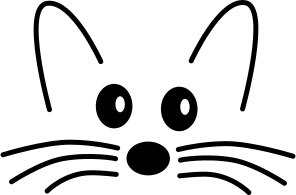
\includegraphics[width=1.4em]{squeak-logo}}}
\newcommand{\dothis}[1]{%
	\medskip
	\noindent\dothisicon
	\ifx#1\empty\else\quad\emph{#1}\fi
	\par\smallskip\nopagebreak}
% NB: To use this in an individual chapter, you must set:
%\graphicspath{{figures/} {../figures/}}
% at the head of the chapter.  Don't forget the final /
%=============================================================
%:Reader hints (hint)
%
% Indicates a non-obvious consequence 
\newcommand{\hint}[1]{\vspace{1ex}\noindent\fbox{\textsc{Astuce}} \emph{#1}}
%=================================================================
% graphics for Morphic handles
\newcommand{\grabHandle}{\raisebox{-0.2ex}{
\includegraphics[width=1em]{blackHandle}}}
\newcommand{\moveHandle}{\raisebox{-0.2ex}{
\includegraphics[width=1em]{moveHandle}}}
\newcommand{\debugHandle}{\raisebox{-0.2ex}{
\includegraphics[width=1em]{debugHandle}}}
% squeak-fr (added for Morphic handles)
\newcommand{\rotateHandle}{\raisebox{-0.2ex}{
\includegraphics[width=1em]{rotateHandle}}}
\newcommand{\viewerHandle}{\raisebox{-0.2ex}{
\includegraphics[width=1em]{viewerHandle}}}
% squeak-fr (add cloverHandle to use \clover in QuickTour.tex as alias
% todo 

%=============================================================
%:Highlighting Important stuff (doublebox)
%
% From Seaside book ...
\newsavebox{\SavedText}
\newlength{\InnerBoxRule}\setlength{\InnerBoxRule}{.75\fboxrule}
\newlength{\OuterBoxRule}\setlength{\OuterBoxRule}{1.5\fboxrule}
\newlength{\BoxSeparation}\setlength{\BoxSeparation}{1.5\fboxrule}
\addtolength{\BoxSeparation}{.5pt}
\newlength{\SaveBoxSep}\setlength{\SaveBoxSep}{2\fboxsep}
%
\newenvironment{doublebox}{\begin{lrbox}{\SavedText}
    \begin{minipage}{.75\textwidth}}
    {\end{minipage}\end{lrbox}\begin{center}
    \setlength{\fboxsep}{\BoxSeparation}\setlength{\fboxrule}{\OuterBoxRule}
    \fbox{\setlength{\fboxsep}{\SaveBoxSep}\setlength{\fboxrule}{\InnerBoxRule}%
      \fbox{\usebox{\SavedText}}}
  \end{center}}
% Use this:
\newcommand{\important}[1]{\begin{doublebox}#1\end{doublebox}}
%=============================================================
%:Section depth
\setcounter{secnumdepth}{2}
%% for this to happen start the file with
%\ifx\wholebook\relax\else
%% $Author$ Martial
% $Date$ Wed Oct 10 13:34:55 CEST 2007
% $Revision$ source: SBE 12715 
% Last Changed Date: 2007-10-08 21:32:45 +0200 (Mon, 08 Oct 2007)
%=============================================================
% NB: documentclass must be set in main document.
% Allows book to be generated in multiple formats.
%=============================================================
%:Packages
\usepackage[french]{babel}
\usepackage[T1]{fontenc}  %%%%%% really important to get the code directly in the text!
\usepackage{lmodern}
%\usepackage[scaled=0.85]{bookmanx} % needs another scale factor if used with \renewcommand{\sfdefault}{cmbr}
\usepackage{palatino}
\usepackage[scaled=0.85]{helvet}
\usepackage{microtype}
\usepackage{graphicx}
\usepackage{theorem}
\usepackage[utf8]{inputenc}
% ON: pdfsync breaks the use of p{width} for tabular columns!
\ifdefined\usepdfsync\usepackage{pdfsync}\fi % Requires texlive 2007
%=============================================================
%:More packages
%Stef should check which ones are used!
%\usepackage{picinpar}
%\usepackage{layout}
%\usepackage{color}
%\usepackage{enum}
%\usepackage{a4wide}
% \usepackage{fancyhdr}
\usepackage{ifthen}
\usepackage{float}
\usepackage{longtable}
\usepackage{makeidx}
\usepackage[nottoc]{tocbibind}
\usepackage{multicol}
\usepackage{booktabs}	% book-style tables
\usepackage{topcapt}	% enables \topcaption
\usepackage{multirow}
\usepackage{tabularx}
%\usepackage[bottom]{footmisc}
\usepackage{xspace}
\usepackage{alltt}
\usepackage{amssymb,textcomp}
\usepackage[usenames,dvipsnames]{color}
%\usepackage{colortbl}
\usepackage[hang]{subfigure}\makeatletter\def\p@subfigure{\thefigure\,}\makeatother
\usepackage{rotating}
\usepackage{enumitem}	% apb: allows more control over tags in enumerations
\usepackage{verbatim}     % for comment environment
\usepackage{varioref}	% for page references that work
\labelformat{footnote}{\thechapter--#1} % to distinguish citations from jurabib
\usepackage{needspace}
\usepackage{isodateo} % enable \isodate
\usepackage[newparttoc]{titlesec}
\usepackage{titletoc}
\usepackage{eurosym}
\usepackage{wrapfig}

\usepackage[
	super,
	citefull=first,
	authorformat={allreversed,and},
	titleformat={commasep,italic}
]{jurabib} % citations as footnotes
\usepackage[
	colorlinks=true,
	linkcolor=black,
	urlcolor=black,
	citecolor=black
]{hyperref}   % should come last

%=============================================================
%:URL style
\makeatletter

\def\url@leostyle{%
  \@ifundefined{selectfont}{\def\UrlFont{\sf}}{\def\UrlFont{\sffamily}}}
% ajouter par Martial pour \traduit (met une dague dans les \doublebox
\def\thempfootnote{\fnsymbol{mpfootnote}}

\makeatother
% Now actually use the newly defined style.
\urlstyle{leo}
%=============================================================
%:Booleans
\newboolean{lulu}
\setboolean{lulu}{false}
\newcommand{\ifluluelse}[2]{\ifthenelse{\boolean{lulu}}{#1}{#2}}
%=============================================================
%:Names
\newcommand{\SUnit}{SUnit\xspace}
\newcommand{\sunit}{SUnit\xspace}
\newcommand{\xUnit}{$x$Unit\xspace}
\newcommand{\JUnit}{JUnit\xspace}
%\newcommand{\XP}{eXtreme Programming\xspace}
\newcommand{\st}{Smalltalk\xspace}
\newcommand{\Squeak}{Squeak\xspace}
\newcommand{\sq}{Squeak\xspace}
\newcommand{\sqmap}{SqueakMap\xspace}
\newcommand{\squeak}{Squeak\xspace}
%\newcommand{\sbe}{\url{scg.unibe.ch/SBE}\xspace}
%\newcommand{\sbe}{\url{squeakbyexample.org}\xspace}
\newcommand{\sbe}{\url{SqueakByExample.org}\xspace}
% squeak-fr: adresse de la version francaise
\newcommand{\spe}{\url{SqueakByExample.org}\xspace} % ?/FR
\newcommand{\sba}{\url{SquareBracketAssociates.org}\xspace}

% squeak-fr: ajout de la \squeakdev pour eviter les problemes de
% changements d'url rencontres dans la VO:
\newcommand{\squeakdev}{\url{www.squeaksource.com/ImageForDevelopers}\xspace} %ou
%\newcommand{\squeakdev}{\url{squeak.ofset.org/squeak-dev}\xspace}

%=============================================================
%:Editorial comment macros
\newcommand{\nnbb}[2]{
    \fbox{\bfseries\sffamily\scriptsize#1}
    {\sf\small$\blacktriangleright$\textit{#2}$\blacktriangleleft$}
   }
\newcommand{\ab}[1]{\nnbb{Andrew}{#1}}
\newcommand{\sd}[1]{\nnbb{St\'{e}f}{#1}}
\newcommand{\md}[1]{\nnbb{Marcus}{#1}}
\newcommand{\on}[1]{\nnbb{Oscar}{#1}}
\newcommand{\damien}[1]{\nnbb{Damien}{#1}}
\newcommand{\lr}[1]{\nnbb{Lukas}{#1}}
\newcommand{\orla}[1]{\nnbb{Orla}{#1}}
%\newcommand{\here}{\nnbb{CONTINUE}{HERE}}
\newcommand{\here}{\nnbb{CONTINUE}{ICI}}

%=============================================================
%:Abbreviation macros
\newcommand{\ie}{\emph{c-\`a-d.}\xspace}
\newcommand{\cad}{\emph{c-\`a-d.}\xspace}
%\newcommand{\eg}{\emph{e.g.},\xspace}
\newcommand{\eg}{\emph{par ex.},\xspace}
\newcommand{\parex}{\emph{par ex.},\xspace}
\newcommand{\etc}{etc\xspace}
%=============================================================
%:Cross reference macros

% [squeak-fr] martial: remarquez les articles devant les noms
\newcommand{\charef}[1]{le chapitre~\ref{cha:#1}\xspace}
% note de martial: utilise dans chapitre Syntax.tex: a redefinir
\newcommand{\charefs}[2]{les chapitres~\ref{cha:#1} et \ref{cha:#2}\xspace}
\newcommand{\secref}[1]{la section~\ref{sec:#1}\xspace}
\newcommand{\figref}[1]{la figure~\ref{fig:#1}\xspace}
\newcommand{\Figref}[1]{La figure~\ref{fig:#1}\xspace}
\newcommand{\appref}[1]{l'annexe~\ref{app:#1}\xspace}
\newcommand{\tabref}[1]{la table~\ref{tab:#1}\xspace}
% defini pour le chapitre Messages.tex
\newcommand{\Tabref}[1]{La table~\ref{tab:#1}\xspace}

% APB: I removed trailing \xspace commands from these macros because
% \xspace mostly doesn't work.  If you want a space after your
% references, type one!
% ON: xspace has always worked just fine for me!  Please leave them in.
%
\newcommand{\ruleref}[1]{\ref{rule:#1}\xspace}
%
\newcommand{\egref}[1]{exemple~\ref{eg:#1}\xspace}
\newcommand{\Egref}[1]{Exemple~\ref{eg:#1}\xspace}
%
\newcommand{\scrref}[1]{script~\ref{scr:#1}\xspace}
\newcommand{\Scrref}[1]{Script~\ref{scr:#1}\xspace}
% t = the
\newcommand{\tscrref}[1]{le script~\ref{scr:#1}\xspace}
\newcommand{\Tscrref}[1]{Le script~\ref{scr:#1}\xspace}
%
\newcommand{\mthref}[1]{m\'ethode~\ref{mth:#1}\xspace}
\newcommand{\mthsref}[1]{m\'ethodes~\ref{mth:#1}\xspace}
\newcommand{\Mthref}[1]{M\'ethode~\ref{mth:#1}\xspace}
\newcommand{\tmthref}[1]{la m\'ethode~\ref{mth:#1}\xspace}
\newcommand{\Tmthref}[1]{La m\'ethode~\ref{mth:#1}\xspace}
%
\newcommand{\clsref}[1]{classe~\ref{cls:#1}\xspace}
\newcommand{\tclsref}[1]{la classe~\ref{cls:#1}\xspace}
\newcommand{\Tclsref}[1]{La classe~\ref{cls:#1}\xspace}
%=============================================================
%:Menu item macro
% for menu items, so we can change our minds on how to print them! (apb)
\definecolor{lightgray}{gray}{0.89}
\newcommand{\menu}[1]{{%
	\setlength{\fboxsep}{0pt}%
	\colorbox{lightgray}{{{\upshape\sffamily\strut \,#1\,}}}}}
% \newcommand{\menu}[1]{{%
% 	\fontfamily{lmr}\selectfont
% 	\upshape\textlangle{\sffamily #1}\textrangle}}
% For submenu items:
\newcommand{\go}{\,$\triangleright$\,}
% \newcommand{\go}{\,$\blacktriangleright$\,}
% For keyboard shortcuts:
%\newcommand{\short}[1]{\mbox{$\langle${\sc CMD}$\rangle$-#1}\xspace}
\newcommand{\short}[1]{\mbox{{\sc cmd}\hspace{0.08em}--\hspace{0.09em}#1}\xspace}
% For buttons:
\newcommand{\button}[1]{{%
	\setlength{\fboxsep}{0pt}%
	\fbox{{\upshape\sffamily\strut \,#1\,}}}}
\newcommand{\toolsflap}{l'onglet \textit{Tools}\xspace}
%=============================================================
%:Reader cues (do this)
%
% Indicate something the reader should try out.
\newcommand{\dothisicon}{\raisebox{-.5ex}{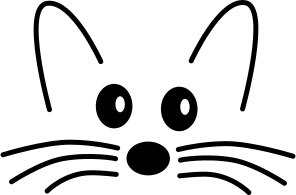
\includegraphics[width=1.4em]{squeak-logo}}}
\newcommand{\dothis}[1]{%
	\medskip
	\noindent\dothisicon
	\ifx#1\empty\else\quad\emph{#1}\fi
	\par\smallskip\nopagebreak}
% NB: To use this in an individual chapter, you must set:
%\graphicspath{{figures/} {../figures/}}
% at the head of the chapter.  Don't forget the final /
%=============================================================
%:Reader hints (hint)
%
% Indicates a non-obvious consequence 
\newcommand{\hint}[1]{\vspace{1ex}\noindent\fbox{\textsc{Astuce}} \emph{#1}}
%=================================================================
% graphics for Morphic handles
\newcommand{\grabHandle}{\raisebox{-0.2ex}{
\includegraphics[width=1em]{blackHandle}}}
\newcommand{\moveHandle}{\raisebox{-0.2ex}{
\includegraphics[width=1em]{moveHandle}}}
\newcommand{\debugHandle}{\raisebox{-0.2ex}{
\includegraphics[width=1em]{debugHandle}}}
% squeak-fr (added for Morphic handles)
\newcommand{\rotateHandle}{\raisebox{-0.2ex}{
\includegraphics[width=1em]{rotateHandle}}}
\newcommand{\viewerHandle}{\raisebox{-0.2ex}{
\includegraphics[width=1em]{viewerHandle}}}
% squeak-fr (add cloverHandle to use \clover in QuickTour.tex as alias
% todo 

%=============================================================
%:Highlighting Important stuff (doublebox)
%
% From Seaside book ...
\newsavebox{\SavedText}
\newlength{\InnerBoxRule}\setlength{\InnerBoxRule}{.75\fboxrule}
\newlength{\OuterBoxRule}\setlength{\OuterBoxRule}{1.5\fboxrule}
\newlength{\BoxSeparation}\setlength{\BoxSeparation}{1.5\fboxrule}
\addtolength{\BoxSeparation}{.5pt}
\newlength{\SaveBoxSep}\setlength{\SaveBoxSep}{2\fboxsep}
%
\newenvironment{doublebox}{\begin{lrbox}{\SavedText}
    \begin{minipage}{.75\textwidth}}
    {\end{minipage}\end{lrbox}\begin{center}
    \setlength{\fboxsep}{\BoxSeparation}\setlength{\fboxrule}{\OuterBoxRule}
    \fbox{\setlength{\fboxsep}{\SaveBoxSep}\setlength{\fboxrule}{\InnerBoxRule}%
      \fbox{\usebox{\SavedText}}}
  \end{center}}
% Use this:
\newcommand{\important}[1]{\begin{doublebox}#1\end{doublebox}}
%=============================================================
%:Section depth
\setcounter{secnumdepth}{2}
%% for this to happen start the file with
%\ifx\wholebook\relax\else
%% $Author$ Martial
% $Date$ Wed Oct 10 13:34:55 CEST 2007
% $Revision$ source: SBE 12715 
% Last Changed Date: 2007-10-08 21:32:45 +0200 (Mon, 08 Oct 2007)
%=============================================================
% NB: documentclass must be set in main document.
% Allows book to be generated in multiple formats.
%=============================================================
%:Packages
\usepackage[french]{babel}
\usepackage[T1]{fontenc}  %%%%%% really important to get the code directly in the text!
\usepackage{lmodern}
%\usepackage[scaled=0.85]{bookmanx} % needs another scale factor if used with \renewcommand{\sfdefault}{cmbr}
\usepackage{palatino}
\usepackage[scaled=0.85]{helvet}
\usepackage{microtype}
\usepackage{graphicx}
\usepackage{theorem}
\usepackage[utf8]{inputenc}
% ON: pdfsync breaks the use of p{width} for tabular columns!
\ifdefined\usepdfsync\usepackage{pdfsync}\fi % Requires texlive 2007
%=============================================================
%:More packages
%Stef should check which ones are used!
%\usepackage{picinpar}
%\usepackage{layout}
%\usepackage{color}
%\usepackage{enum}
%\usepackage{a4wide}
% \usepackage{fancyhdr}
\usepackage{ifthen}
\usepackage{float}
\usepackage{longtable}
\usepackage{makeidx}
\usepackage[nottoc]{tocbibind}
\usepackage{multicol}
\usepackage{booktabs}	% book-style tables
\usepackage{topcapt}	% enables \topcaption
\usepackage{multirow}
\usepackage{tabularx}
%\usepackage[bottom]{footmisc}
\usepackage{xspace}
\usepackage{alltt}
\usepackage{amssymb,textcomp}
\usepackage[usenames,dvipsnames]{color}
%\usepackage{colortbl}
\usepackage[hang]{subfigure}\makeatletter\def\p@subfigure{\thefigure\,}\makeatother
\usepackage{rotating}
\usepackage{enumitem}	% apb: allows more control over tags in enumerations
\usepackage{verbatim}     % for comment environment
\usepackage{varioref}	% for page references that work
\labelformat{footnote}{\thechapter--#1} % to distinguish citations from jurabib
\usepackage{needspace}
\usepackage{isodateo} % enable \isodate
\usepackage[newparttoc]{titlesec}
\usepackage{titletoc}
\usepackage{eurosym}
\usepackage{wrapfig}

\usepackage[
	super,
	citefull=first,
	authorformat={allreversed,and},
	titleformat={commasep,italic}
]{jurabib} % citations as footnotes
\usepackage[
	colorlinks=true,
	linkcolor=black,
	urlcolor=black,
	citecolor=black
]{hyperref}   % should come last

%=============================================================
%:URL style
\makeatletter

\def\url@leostyle{%
  \@ifundefined{selectfont}{\def\UrlFont{\sf}}{\def\UrlFont{\sffamily}}}
% ajouter par Martial pour \traduit (met une dague dans les \doublebox
\def\thempfootnote{\fnsymbol{mpfootnote}}

\makeatother
% Now actually use the newly defined style.
\urlstyle{leo}
%=============================================================
%:Booleans
\newboolean{lulu}
\setboolean{lulu}{false}
\newcommand{\ifluluelse}[2]{\ifthenelse{\boolean{lulu}}{#1}{#2}}
%=============================================================
%:Names
\newcommand{\SUnit}{SUnit\xspace}
\newcommand{\sunit}{SUnit\xspace}
\newcommand{\xUnit}{$x$Unit\xspace}
\newcommand{\JUnit}{JUnit\xspace}
%\newcommand{\XP}{eXtreme Programming\xspace}
\newcommand{\st}{Smalltalk\xspace}
\newcommand{\Squeak}{Squeak\xspace}
\newcommand{\sq}{Squeak\xspace}
\newcommand{\sqmap}{SqueakMap\xspace}
\newcommand{\squeak}{Squeak\xspace}
%\newcommand{\sbe}{\url{scg.unibe.ch/SBE}\xspace}
%\newcommand{\sbe}{\url{squeakbyexample.org}\xspace}
\newcommand{\sbe}{\url{SqueakByExample.org}\xspace}
% squeak-fr: adresse de la version francaise
\newcommand{\spe}{\url{SqueakByExample.org}\xspace} % ?/FR
\newcommand{\sba}{\url{SquareBracketAssociates.org}\xspace}

% squeak-fr: ajout de la \squeakdev pour eviter les problemes de
% changements d'url rencontres dans la VO:
\newcommand{\squeakdev}{\url{www.squeaksource.com/ImageForDevelopers}\xspace} %ou
%\newcommand{\squeakdev}{\url{squeak.ofset.org/squeak-dev}\xspace}

%=============================================================
%:Editorial comment macros
\newcommand{\nnbb}[2]{
    \fbox{\bfseries\sffamily\scriptsize#1}
    {\sf\small$\blacktriangleright$\textit{#2}$\blacktriangleleft$}
   }
\newcommand{\ab}[1]{\nnbb{Andrew}{#1}}
\newcommand{\sd}[1]{\nnbb{St\'{e}f}{#1}}
\newcommand{\md}[1]{\nnbb{Marcus}{#1}}
\newcommand{\on}[1]{\nnbb{Oscar}{#1}}
\newcommand{\damien}[1]{\nnbb{Damien}{#1}}
\newcommand{\lr}[1]{\nnbb{Lukas}{#1}}
\newcommand{\orla}[1]{\nnbb{Orla}{#1}}
%\newcommand{\here}{\nnbb{CONTINUE}{HERE}}
\newcommand{\here}{\nnbb{CONTINUE}{ICI}}

%=============================================================
%:Abbreviation macros
\newcommand{\ie}{\emph{c-\`a-d.}\xspace}
\newcommand{\cad}{\emph{c-\`a-d.}\xspace}
%\newcommand{\eg}{\emph{e.g.},\xspace}
\newcommand{\eg}{\emph{par ex.},\xspace}
\newcommand{\parex}{\emph{par ex.},\xspace}
\newcommand{\etc}{etc\xspace}
%=============================================================
%:Cross reference macros

% [squeak-fr] martial: remarquez les articles devant les noms
\newcommand{\charef}[1]{le chapitre~\ref{cha:#1}\xspace}
% note de martial: utilise dans chapitre Syntax.tex: a redefinir
\newcommand{\charefs}[2]{les chapitres~\ref{cha:#1} et \ref{cha:#2}\xspace}
\newcommand{\secref}[1]{la section~\ref{sec:#1}\xspace}
\newcommand{\figref}[1]{la figure~\ref{fig:#1}\xspace}
\newcommand{\Figref}[1]{La figure~\ref{fig:#1}\xspace}
\newcommand{\appref}[1]{l'annexe~\ref{app:#1}\xspace}
\newcommand{\tabref}[1]{la table~\ref{tab:#1}\xspace}
% defini pour le chapitre Messages.tex
\newcommand{\Tabref}[1]{La table~\ref{tab:#1}\xspace}

% APB: I removed trailing \xspace commands from these macros because
% \xspace mostly doesn't work.  If you want a space after your
% references, type one!
% ON: xspace has always worked just fine for me!  Please leave them in.
%
\newcommand{\ruleref}[1]{\ref{rule:#1}\xspace}
%
\newcommand{\egref}[1]{exemple~\ref{eg:#1}\xspace}
\newcommand{\Egref}[1]{Exemple~\ref{eg:#1}\xspace}
%
\newcommand{\scrref}[1]{script~\ref{scr:#1}\xspace}
\newcommand{\Scrref}[1]{Script~\ref{scr:#1}\xspace}
% t = the
\newcommand{\tscrref}[1]{le script~\ref{scr:#1}\xspace}
\newcommand{\Tscrref}[1]{Le script~\ref{scr:#1}\xspace}
%
\newcommand{\mthref}[1]{m\'ethode~\ref{mth:#1}\xspace}
\newcommand{\mthsref}[1]{m\'ethodes~\ref{mth:#1}\xspace}
\newcommand{\Mthref}[1]{M\'ethode~\ref{mth:#1}\xspace}
\newcommand{\tmthref}[1]{la m\'ethode~\ref{mth:#1}\xspace}
\newcommand{\Tmthref}[1]{La m\'ethode~\ref{mth:#1}\xspace}
%
\newcommand{\clsref}[1]{classe~\ref{cls:#1}\xspace}
\newcommand{\tclsref}[1]{la classe~\ref{cls:#1}\xspace}
\newcommand{\Tclsref}[1]{La classe~\ref{cls:#1}\xspace}
%=============================================================
%:Menu item macro
% for menu items, so we can change our minds on how to print them! (apb)
\definecolor{lightgray}{gray}{0.89}
\newcommand{\menu}[1]{{%
	\setlength{\fboxsep}{0pt}%
	\colorbox{lightgray}{{{\upshape\sffamily\strut \,#1\,}}}}}
% \newcommand{\menu}[1]{{%
% 	\fontfamily{lmr}\selectfont
% 	\upshape\textlangle{\sffamily #1}\textrangle}}
% For submenu items:
\newcommand{\go}{\,$\triangleright$\,}
% \newcommand{\go}{\,$\blacktriangleright$\,}
% For keyboard shortcuts:
%\newcommand{\short}[1]{\mbox{$\langle${\sc CMD}$\rangle$-#1}\xspace}
\newcommand{\short}[1]{\mbox{{\sc cmd}\hspace{0.08em}--\hspace{0.09em}#1}\xspace}
% For buttons:
\newcommand{\button}[1]{{%
	\setlength{\fboxsep}{0pt}%
	\fbox{{\upshape\sffamily\strut \,#1\,}}}}
\newcommand{\toolsflap}{l'onglet \textit{Tools}\xspace}
%=============================================================
%:Reader cues (do this)
%
% Indicate something the reader should try out.
\newcommand{\dothisicon}{\raisebox{-.5ex}{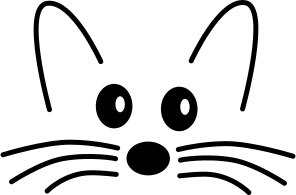
\includegraphics[width=1.4em]{squeak-logo}}}
\newcommand{\dothis}[1]{%
	\medskip
	\noindent\dothisicon
	\ifx#1\empty\else\quad\emph{#1}\fi
	\par\smallskip\nopagebreak}
% NB: To use this in an individual chapter, you must set:
%\graphicspath{{figures/} {../figures/}}
% at the head of the chapter.  Don't forget the final /
%=============================================================
%:Reader hints (hint)
%
% Indicates a non-obvious consequence 
\newcommand{\hint}[1]{\vspace{1ex}\noindent\fbox{\textsc{Astuce}} \emph{#1}}
%=================================================================
% graphics for Morphic handles
\newcommand{\grabHandle}{\raisebox{-0.2ex}{
\includegraphics[width=1em]{blackHandle}}}
\newcommand{\moveHandle}{\raisebox{-0.2ex}{
\includegraphics[width=1em]{moveHandle}}}
\newcommand{\debugHandle}{\raisebox{-0.2ex}{
\includegraphics[width=1em]{debugHandle}}}
% squeak-fr (added for Morphic handles)
\newcommand{\rotateHandle}{\raisebox{-0.2ex}{
\includegraphics[width=1em]{rotateHandle}}}
\newcommand{\viewerHandle}{\raisebox{-0.2ex}{
\includegraphics[width=1em]{viewerHandle}}}
% squeak-fr (add cloverHandle to use \clover in QuickTour.tex as alias
% todo 

%=============================================================
%:Highlighting Important stuff (doublebox)
%
% From Seaside book ...
\newsavebox{\SavedText}
\newlength{\InnerBoxRule}\setlength{\InnerBoxRule}{.75\fboxrule}
\newlength{\OuterBoxRule}\setlength{\OuterBoxRule}{1.5\fboxrule}
\newlength{\BoxSeparation}\setlength{\BoxSeparation}{1.5\fboxrule}
\addtolength{\BoxSeparation}{.5pt}
\newlength{\SaveBoxSep}\setlength{\SaveBoxSep}{2\fboxsep}
%
\newenvironment{doublebox}{\begin{lrbox}{\SavedText}
    \begin{minipage}{.75\textwidth}}
    {\end{minipage}\end{lrbox}\begin{center}
    \setlength{\fboxsep}{\BoxSeparation}\setlength{\fboxrule}{\OuterBoxRule}
    \fbox{\setlength{\fboxsep}{\SaveBoxSep}\setlength{\fboxrule}{\InnerBoxRule}%
      \fbox{\usebox{\SavedText}}}
  \end{center}}
% Use this:
\newcommand{\important}[1]{\begin{doublebox}#1\end{doublebox}}
%=============================================================
%:Section depth
\setcounter{secnumdepth}{2}
%% for this to happen start the file with
%\ifx\wholebook\relax\else
%\input{../common.tex}
%\begin{document}
%\fi
% and terminate by
% \ifx\wholebook\relax\else\end{document}\fi

\DeclareGraphicsExtensions{.pdf, .jpg, .png}
%=============================================================
%:PDF setup
\hypersetup{
%   a4paper,
%   pdfstartview=FitV,
%   colorlinks,
%   linkcolor=darkblue,
%   citecolor=darkblue,
%   pdftitle={Squeak by Example},
pdftitle={Squeak par l'exemple},
   pdfauthor={Andrew Black, St\'ephane Ducasse,	Oscar Nierstrasz,
Damien Pollet},
   pdfkeywords={Smalltalk, Squeak, Programmation Orient\'ee Objet},
pdfsubject={Informatique, Computer Science}
}
%=============================================================
%:Page layout and appearance
%
% \renewcommand{\headrulewidth}{0pt}
\renewcommand{\chaptermark}[1]{\markboth{#1}{}}
\renewcommand{\sectionmark}[1]{\markright{\thesection\ #1}}
\renewpagestyle{plain}[\small\itshape]{%
	\setheadrule{0pt}%
	\sethead[\thepage][][]{}{}{\thepage}%
	\setfoot[][][]{}{}{}}
\renewpagestyle{headings}[\small\itshape]{%
	\setheadrule{0pt}%
	\setmarks{chapter}{section}%
	\sethead[\thepage][][\chaptertitle]{\sectiontitle}{}{\thepage}%
	\setfoot[][][]{}{}{}}
%=============================================================
%:Title section setup and TOC numbering depth
\setcounter{secnumdepth}{1}
\setcounter{tocdepth}{1}
\titleformat{\part}[display]{\centering}{\huge\partname\ \thepart}{1em}{\Huge\textbf}[]
\titleformat{\chapter}[display]{}{\huge\chaptertitlename\ \thechapter}{1em}{\Huge\raggedright\textbf}[]
\titlecontents{part}[3pc]{%
		\pagebreak[2]\addvspace{1em plus.4em minus.2em}%
		\leavevmode\large\bfseries}
	{\contentslabel{3pc}}{\hspace*{-3pc}}
	{}[\nopagebreak]
\titlecontents{chapter}[3pc]{%
		\pagebreak[0]\addvspace{1em plus.2em minus.2em}%
		\leavevmode\bfseries}
	{\contentslabel{3pc}}{}
	{\hfill\contentspage}[\nopagebreak]
\dottedcontents{section}[3pc]{}{3pc}{1pc}
\dottedcontents{subsection}[3pc]{}{0pc}{1pc}
% \dottedcontents{subsection}[4.5em]{}{0pt}{1pc}
% Make \cleardoublepage insert really blank pages http://www.tex.ac.uk/cgi-bin/texfaq2html?label=reallyblank
\let\origdoublepage\cleardoublepage
\newcommand{\clearemptydoublepage}{%
  \clearpage
  {\pagestyle{empty}\origdoublepage}}
\let\cleardoublepage\clearemptydoublepage % see http://www.tex.ac.uk/cgi-bin/texfaq2html?label=patch
%=============================================================
%:FAQ macros (for FAQ chapter)
\newtheorem{faq}{FAQ}
\newcommand{\answer}{\paragraph{R\'eponse}\ }
%=============================================================
%:Listings package configuration
\usepackage{listings}
\newcommand{\caret}{\makebox{\raisebox{0.4ex}{\footnotesize{$\wedge$}}}}
\lstdefinelanguage{Smalltalk}{
%  morekeywords={self,super,true,false,nil,thisContext}, % This is overkill
  morestring=[d]',
  morecomment=[s]{"}{"},
  alsoletter={\#:},
  escapechar={!},
  escapebegin=\itshape, % comment-like by default (Martial 11/2007)
  literate=
    {BANG}{!}1
    {UNDERSCORE}{\_}1
    {\\st}{Smalltalk}9 % convenience -- in case \st occurs in code
    % {'}{{\textquotesingle}}1 % replaced by upquote=true in \lstset
    {_}{{$\leftarrow$}}1
    {>>>}{{\sep}}1
    {^}{{$\uparrow$}}1
    {~}{{$\sim$}}1
    {-}{{\sf -\hspace{-0.13em}-}}1  % the goal is to make - the same width as +
    {+}{\raisebox{0.08ex}{+}}1		% and to raise + off the baseline to match -
    {-->}{{\quad$\longrightarrow$\quad}}3
	, % Don't forget the comma at the end!
  tabsize=4
}[keywords,comments,strings]
% ajout pour les échappements dans les codes
% indispensable pour mettre le code en emphase (cf. Model.tex) 
\newcommand{\codeify}[1]{\NoAutoSpaceBeforeFDP#1\AutoSpaceBeforeFDP}
\newcommand{\normcomment}[1]{\emph{#1}} %cf. Streams
\newcommand{\normcode}[1]{\emph{\codeify{#1}}} %cf. Streams
\newcommand{\emcode}[1]{\textbf{\normcode{#1}}} % Martial 11/2007
\lstset{language=Smalltalk,
	basicstyle=\sffamily,
	keywordstyle=\color{black}\bfseries,
	% stringstyle=\ttfamily, % Ugly! do we really want this? -- on
	%commentstyle=\itshape,
	mathescape=true,
	showstringspaces=false,
	keepspaces=true,
	breaklines=true,
	breakautoindent=true,
	lineskip={-1pt}, % Ugly hack
	upquote=true, % straight quote; requires textcomp package
	columns=fullflexible} % no fixed width fonts
% In-line code (literal)
% Normally use this for all in-line code:
\newcommand{\ct}{\lstinline[mathescape=false,basicstyle={\sffamily\upshape}]}
% apb 2007.8.28 added the \upshape declaration to avoid getting italicized code in \dothis{ } sections.
% In-line code (latex enabled)
% Use this only in special situations where \ct does not work
% (within section headings ...):

% [squeak-fr] Modification de \lct suivant les indications de Martial Boniou
\newcommand{\lct}[1]{\textsf{\textup{\NoAutoSpaceBeforeFDP #1
\AutoSpaceBeforeFDP}}} %\xspace

% Use these for system categories and protocols:
\newcommand{\scat}[1]{\emph{\textsf{#1}}\xspace}
\newcommand{\pkg}[1]{\emph{\textsf{#1}}\xspace}
\newcommand{\prot}[1]{\emph{\textsf{#1}}\xspace}
% Code environments
% NB: the arg is for tests
% Only code and example environments may be tests
\lstnewenvironment{code}[1]{%
	\lstset{%
		frame=lines,
		mathescape=false
	}
}{}
\def\ignoredollar#1{}
%=============================================================
%:Code environments (method, script ...)
% NB: the third arg is for tests
% Only code and example environments may be tests
\lstnewenvironment{example}[3][defaultlabel]{%
	\renewcommand{\lstlistingname}{Exemple}%
	\lstset{
		frame=lines,
		mathescape=false,
		caption={\emph{#2}},
		label={eg:#1}
	}
}{}
\lstnewenvironment{script}[2][defaultlabel]{%
\renewcommand{\lstlistingname}{Script}%
	\lstset{
		frame=lines,
		mathescape=false,
		name={Script},
		caption={\emph{#2}},
		label={scr:#1}
	}
}{}
\lstnewenvironment{method}[2][defaultlabel]{%
	\renewcommand{\lstlistingname}{M\'ethode}%
	\lstset{
		frame=lines,
		mathescape=false,
		name={M\'ethode},
		caption={\emph{#2}},
		label={mth:#1}
	}
}{}
\lstnewenvironment{methods}[2][defaultlabel]{% just for multiple methods at once
	\renewcommand{\lstlistingname}{M\'ethodes}%
	\lstset{
		frame=lines,
		mathescape=false,
		name={M\'ethode},
		caption={\emph{#2}},
		label={mth:#1}
	}
}{}
\lstnewenvironment{numMethod}[2][defaultlabel]{%
	\renewcommand{\lstlistingname}{M\'ethode}%
	\lstset{
		numbers=left,
		numberstyle={\tiny\sffamily},
		frame=lines,
		mathescape=false,
		name={M\'ethode},
		caption={\emph{#2}},
		label={mth:#1}
	}
}{}
\lstnewenvironment{classdef}[2][defaultlabel]{%
	\renewcommand{\lstlistingname}{Classe}%
	\lstset{
		frame=lines,
		mathescape=false,
		name={Classe},
		caption={\emph{#2}},
		label={cls:#1}
	}
}{}
%=============================================================
%:Reserving space
% Usually need one more line than the actual lines of code
\newcommand{\needlines}[1]{\Needspace{#1\baselineskip}}
%=============================================================
%:Indexing macros
% Macros ending with "ind" generate text as well as an index entry
% Macros ending with "index" *only* generate an index entry
\newcommand{\ind}[1]{\index{#1}#1\xspace} % plain text
\newcommand{\subind}[2]{\index{#1!#2}#2\xspace} % show #2, subindex inder #1
\newcommand{\emphind}[1]{\index{#1}\emph{#1}\xspace} % emph #1
\newcommand{\emphsubind}[2]{\index{#1!#2}\emph{#2}\xspace} % show emph #2, subindex inder #1
\newcommand{\scatind}[1]{\index{#1@\textsf{#1} (cat\'egorie)}\scat{#1}} % category
\newcommand{\protind}[1]{\index{#1@\textsf{#1} (protocole)}\prot{#1}} % protocol
% \newcommand{\clsind}[1]{\index{#1@\textsf{#1} (class)}\ct{#1}\xspace}
\newcommand{\clsind}[1]{\index{#1!\#@(classe)}\ct{#1}\xspace} % class
\newcommand{\cvind}[1]{\index{#1@\textsf{#1} (variable de classe)}\ct{#1}\xspace} % class var
\newcommand{\glbind}[1]{\index{#1@\textsf{#1} (globale)}\ct{#1}\xspace} % global
\newcommand{\patind}[1]{\index{#1@#1 (patron)}\ct{#1}\xspace} % pattern
\newcommand{\pvind}[1]{\index{#1@\textsf{#1} (pseudo-variable)}\ct{#1}\xspace} % pseudo variable
% [squeak - fr]Martial: I found the following cleaner (should be
% merged in SBE for self and super)
\newcommand{\subpvindex}[2]{\index{#1@\textsf{#1} (pseudo-variable)!#2}}
\newcommand{\subpvind}[2]{\index{#1@\textsf{#1} (pseudo-variable)!#2}#2\xspace}
% used in Model.tex
\newcommand{\mthind}[2]{\index{#1!#2@\ct{#2}}\ct{#2}\xspace} % show method name only
\newcommand{\lmthind}[2]{\index{#1!#2@\ct{#2}}\lct{#2}\xspace} % show method name only
\newcommand{\cmind}[2]{\index{#1!#2@\ct{#2}}\ct{#1>>>#2}\xspace} % show class>>method
\newcommand{\toolsflapind}{\index{onglet Tools}\toolsflap} % index tools flap
% The following only generate an index entry:
% \newcommand{\clsindex}[1]{\index{#1@\textsf{#1} (class)}}
\newcommand{\clsindex}[1]{\index{#1!\#@(classe)}} % class
\newcommand{\cmindex}[2]{\index{#1!#2@\ct{#2}}} % class>>method
\newcommand{\cvindex}[1]{\index{#1@\textsf{#1} (variable de classe)}} % class var
\newcommand{\glbindex}[1]{\index{#1@\textsf{#1} (globale)}}% global
\newcommand{\pvindex}[1]{\index{#1@\textsf{#1} (pseudo-variable)}}% pseudo var
\newcommand{\seeindex}[2]{\index{#1|see{#2}}} % #1, see #2
\newcommand{\scatindex}[1]{\index{#1@\textsf{#1} (cat\'egorie)}} % category
\newcommand{\protindex}[1]{\index{#1@\textsf{#1} (protocole)}} % protocol
% How can we have the main entry page numbers in bold yet not break the hyperlink?
\newcommand{\boldidx}[1]{{\bf #1}} % breaks hyperlink
%\newcommand{\indmain}[1]{\index{#1|boldidx}#1\xspace} % plain text, main entry
%\newcommand{\emphsubindmain}[2]{\index{#1!#2|boldidx}\emph{#2}\xspace} % subindex, main entry
%\newcommand{\subindmain}[2]{\index{#1!#2|boldidx}#2\xspace} % subindex, main entry
%\newcommand{\clsindmain}[1]{\index{#1@\textsf{#1} (class)|boldidx}\ct{#1}\xspace}
%\newcommand{\clsindmain}[1]{\index{#1!\#@(class)|boldidx}\ct{#1}\xspace} % class main
%\newcommand{\indexmain}[1]{\index{#1|boldidx}} % main index entry only
\newcommand{\indmain}[1]{\index{#1}#1\xspace} 
\newcommand{\emphsubindmain}[2]{\index{#1!#2}\emph{#2}\xspace} % subindex, main entry
\newcommand{\subindmain}[2]{\index{#1!#2}#2\xspace} % subindex, main entry
%\newcommand{\clsindmain}[1]{\index{#1@\textsf{#1} (class)}\ct{#1}\xspace}
\newcommand{\clsindmain}[1]{\index{#1!\#@(classe)}\ct{#1}\xspace} % class main
\newcommand{\indexmain}[1]{\index{#1}} 
%=============================================================
%:Code macros
% some constants
\newcommand{\codesize}{\small}
\newcommand{\codefont}{\sffamily}
\newcommand{\cat}[1]{\textit{Dans la cat\'egorie #1}}%%To remove later
\newlength{\scriptindent}
\setlength{\scriptindent}{.3cm}
%% Method presentation constants
\newlength{\methodindent}
\newlength{\methodwordlength}
\newlength{\aftermethod}
\setlength{\methodindent}{0.2cm}
\settowidth{\methodwordlength}{\ M\'ethode\ }
%=============================================================
%:Smalltalk macros
%\newcommand{\sep}{{$\gg$}}
\newcommand{\sep}{\mbox{>>}}
\newcommand{\self}{\ct{self}\xspace}
\newcommand{\super}{\ct{super}\xspace}
\newcommand{\nil}{\ct{nil}\xspace}
%=============================================================
% be less conservative about float placement
% these commands are from http://www.tex.ac.uk/cgi-bin/texfaq2html?label=floats
\renewcommand{\topfraction}{.9}
\renewcommand{\bottomfraction}{.9}
\renewcommand{\textfraction}{.1}
\renewcommand{\floatpagefraction}{.85}
\renewcommand{\dbltopfraction}{.66}
\renewcommand{\dblfloatpagefraction}{.85}
\setcounter{topnumber}{9}
\setcounter{bottomnumber}{9}
\setcounter{totalnumber}{20}
\setcounter{dbltopnumber}{9}
%=============================================================
%% [Squeak-fr]
% pour identifier les zones de texte à corriger d'urgence!
\newcommand{\arevoir}[1]{#1}
% \traduit utilisé dans Model.tex
\newcommand{\traduit}[1]{\footnote[2]{#1}}
% changeset alias
\newcommand{\changeset}{\emph{change set}\xspace}
\newcommand{\changesets}{\emph{change sets}\xspace}
% callback alias
\newcommand{\callback}{\emph{callback}\xspace}
% blobmorph alias (QuickTour->blob)
\newcommand{\blobmorph}{\emph{blob}\xspace}
% repository
\newcommand{\squeaksource}{\textsf{SqueakSource}\xspace}
\newcommand{\sourceforge}{\textsf{SourceForge}\xspace}
% L'onglet Tools
\newcommand{\Toolsflap}{L'onglet \textit{Tools}\xspace}
% Mac OS X
\newcommand{\macosx}{\mbox{Mac OS X}\xspace}
% code en francais (uniquement dans le chapitre BasicClasses)
\newcommand{\codefrench}[1]{\NoAutoSpaceBeforeFDP\texttt{#1}\AutoSpaceBeforeFDP\xspace}
% mantra du modele objet (suite a l'erreur de martial)
\newcommand{\Mantra}{Tout est objet\xspace}
\newcommand{\mantra}{\MakeLowercase{\Mantra}\xspace}
% césure
\hyphenation{Omni-Brow-ser}
\hyphenation{m\'e-tho-de} % erreur de cesure commune
\hyphenation{m\'e-tho-des}
\hyphenation{e-xem-ple}
\hyphenation{en-re-gi-stre}
\hyphenation{a-na-ly-seur}
\hyphenation{glo-ba-le}
\hyphenation{fi-gu-re}
\hyphenation{vi-si-bles}
\hyphenation{cor-res-pon-dan-te}
\hyphenation{Work-space}
%=============================================================
% apb doesn't like paragraphs to run in to each other without a break
\parskip 1ex
%=============================================================
%:Stuff to check, merge or deprecate
%\setlength{\marginparsep}{2mm}
%\renewcommand{\baselinestretch}{1.1}
%=============================================================

%\begin{document}
%\fi
% and terminate by
% \ifx\wholebook\relax\else\end{document}\fi

\DeclareGraphicsExtensions{.pdf, .jpg, .png}
%=============================================================
%:PDF setup
\hypersetup{
%   a4paper,
%   pdfstartview=FitV,
%   colorlinks,
%   linkcolor=darkblue,
%   citecolor=darkblue,
%   pdftitle={Squeak by Example},
pdftitle={Squeak par l'exemple},
   pdfauthor={Andrew Black, St\'ephane Ducasse,	Oscar Nierstrasz,
Damien Pollet},
   pdfkeywords={Smalltalk, Squeak, Programmation Orient\'ee Objet},
pdfsubject={Informatique, Computer Science}
}
%=============================================================
%:Page layout and appearance
%
% \renewcommand{\headrulewidth}{0pt}
\renewcommand{\chaptermark}[1]{\markboth{#1}{}}
\renewcommand{\sectionmark}[1]{\markright{\thesection\ #1}}
\renewpagestyle{plain}[\small\itshape]{%
	\setheadrule{0pt}%
	\sethead[\thepage][][]{}{}{\thepage}%
	\setfoot[][][]{}{}{}}
\renewpagestyle{headings}[\small\itshape]{%
	\setheadrule{0pt}%
	\setmarks{chapter}{section}%
	\sethead[\thepage][][\chaptertitle]{\sectiontitle}{}{\thepage}%
	\setfoot[][][]{}{}{}}
%=============================================================
%:Title section setup and TOC numbering depth
\setcounter{secnumdepth}{1}
\setcounter{tocdepth}{1}
\titleformat{\part}[display]{\centering}{\huge\partname\ \thepart}{1em}{\Huge\textbf}[]
\titleformat{\chapter}[display]{}{\huge\chaptertitlename\ \thechapter}{1em}{\Huge\raggedright\textbf}[]
\titlecontents{part}[3pc]{%
		\pagebreak[2]\addvspace{1em plus.4em minus.2em}%
		\leavevmode\large\bfseries}
	{\contentslabel{3pc}}{\hspace*{-3pc}}
	{}[\nopagebreak]
\titlecontents{chapter}[3pc]{%
		\pagebreak[0]\addvspace{1em plus.2em minus.2em}%
		\leavevmode\bfseries}
	{\contentslabel{3pc}}{}
	{\hfill\contentspage}[\nopagebreak]
\dottedcontents{section}[3pc]{}{3pc}{1pc}
\dottedcontents{subsection}[3pc]{}{0pc}{1pc}
% \dottedcontents{subsection}[4.5em]{}{0pt}{1pc}
% Make \cleardoublepage insert really blank pages http://www.tex.ac.uk/cgi-bin/texfaq2html?label=reallyblank
\let\origdoublepage\cleardoublepage
\newcommand{\clearemptydoublepage}{%
  \clearpage
  {\pagestyle{empty}\origdoublepage}}
\let\cleardoublepage\clearemptydoublepage % see http://www.tex.ac.uk/cgi-bin/texfaq2html?label=patch
%=============================================================
%:FAQ macros (for FAQ chapter)
\newtheorem{faq}{FAQ}
\newcommand{\answer}{\paragraph{R\'eponse}\ }
%=============================================================
%:Listings package configuration
\usepackage{listings}
\newcommand{\caret}{\makebox{\raisebox{0.4ex}{\footnotesize{$\wedge$}}}}
\lstdefinelanguage{Smalltalk}{
%  morekeywords={self,super,true,false,nil,thisContext}, % This is overkill
  morestring=[d]',
  morecomment=[s]{"}{"},
  alsoletter={\#:},
  escapechar={!},
  escapebegin=\itshape, % comment-like by default (Martial 11/2007)
  literate=
    {BANG}{!}1
    {UNDERSCORE}{\_}1
    {\\st}{Smalltalk}9 % convenience -- in case \st occurs in code
    % {'}{{\textquotesingle}}1 % replaced by upquote=true in \lstset
    {_}{{$\leftarrow$}}1
    {>>>}{{\sep}}1
    {^}{{$\uparrow$}}1
    {~}{{$\sim$}}1
    {-}{{\sf -\hspace{-0.13em}-}}1  % the goal is to make - the same width as +
    {+}{\raisebox{0.08ex}{+}}1		% and to raise + off the baseline to match -
    {-->}{{\quad$\longrightarrow$\quad}}3
	, % Don't forget the comma at the end!
  tabsize=4
}[keywords,comments,strings]
% ajout pour les échappements dans les codes
% indispensable pour mettre le code en emphase (cf. Model.tex) 
\newcommand{\codeify}[1]{\NoAutoSpaceBeforeFDP#1\AutoSpaceBeforeFDP}
\newcommand{\normcomment}[1]{\emph{#1}} %cf. Streams
\newcommand{\normcode}[1]{\emph{\codeify{#1}}} %cf. Streams
\newcommand{\emcode}[1]{\textbf{\normcode{#1}}} % Martial 11/2007
\lstset{language=Smalltalk,
	basicstyle=\sffamily,
	keywordstyle=\color{black}\bfseries,
	% stringstyle=\ttfamily, % Ugly! do we really want this? -- on
	%commentstyle=\itshape,
	mathescape=true,
	showstringspaces=false,
	keepspaces=true,
	breaklines=true,
	breakautoindent=true,
	lineskip={-1pt}, % Ugly hack
	upquote=true, % straight quote; requires textcomp package
	columns=fullflexible} % no fixed width fonts
% In-line code (literal)
% Normally use this for all in-line code:
\newcommand{\ct}{\lstinline[mathescape=false,basicstyle={\sffamily\upshape}]}
% apb 2007.8.28 added the \upshape declaration to avoid getting italicized code in \dothis{ } sections.
% In-line code (latex enabled)
% Use this only in special situations where \ct does not work
% (within section headings ...):

% [squeak-fr] Modification de \lct suivant les indications de Martial Boniou
\newcommand{\lct}[1]{\textsf{\textup{\NoAutoSpaceBeforeFDP #1
\AutoSpaceBeforeFDP}}} %\xspace

% Use these for system categories and protocols:
\newcommand{\scat}[1]{\emph{\textsf{#1}}\xspace}
\newcommand{\pkg}[1]{\emph{\textsf{#1}}\xspace}
\newcommand{\prot}[1]{\emph{\textsf{#1}}\xspace}
% Code environments
% NB: the arg is for tests
% Only code and example environments may be tests
\lstnewenvironment{code}[1]{%
	\lstset{%
		frame=lines,
		mathescape=false
	}
}{}
\def\ignoredollar#1{}
%=============================================================
%:Code environments (method, script ...)
% NB: the third arg is for tests
% Only code and example environments may be tests
\lstnewenvironment{example}[3][defaultlabel]{%
	\renewcommand{\lstlistingname}{Exemple}%
	\lstset{
		frame=lines,
		mathescape=false,
		caption={\emph{#2}},
		label={eg:#1}
	}
}{}
\lstnewenvironment{script}[2][defaultlabel]{%
\renewcommand{\lstlistingname}{Script}%
	\lstset{
		frame=lines,
		mathescape=false,
		name={Script},
		caption={\emph{#2}},
		label={scr:#1}
	}
}{}
\lstnewenvironment{method}[2][defaultlabel]{%
	\renewcommand{\lstlistingname}{M\'ethode}%
	\lstset{
		frame=lines,
		mathescape=false,
		name={M\'ethode},
		caption={\emph{#2}},
		label={mth:#1}
	}
}{}
\lstnewenvironment{methods}[2][defaultlabel]{% just for multiple methods at once
	\renewcommand{\lstlistingname}{M\'ethodes}%
	\lstset{
		frame=lines,
		mathescape=false,
		name={M\'ethode},
		caption={\emph{#2}},
		label={mth:#1}
	}
}{}
\lstnewenvironment{numMethod}[2][defaultlabel]{%
	\renewcommand{\lstlistingname}{M\'ethode}%
	\lstset{
		numbers=left,
		numberstyle={\tiny\sffamily},
		frame=lines,
		mathescape=false,
		name={M\'ethode},
		caption={\emph{#2}},
		label={mth:#1}
	}
}{}
\lstnewenvironment{classdef}[2][defaultlabel]{%
	\renewcommand{\lstlistingname}{Classe}%
	\lstset{
		frame=lines,
		mathescape=false,
		name={Classe},
		caption={\emph{#2}},
		label={cls:#1}
	}
}{}
%=============================================================
%:Reserving space
% Usually need one more line than the actual lines of code
\newcommand{\needlines}[1]{\Needspace{#1\baselineskip}}
%=============================================================
%:Indexing macros
% Macros ending with "ind" generate text as well as an index entry
% Macros ending with "index" *only* generate an index entry
\newcommand{\ind}[1]{\index{#1}#1\xspace} % plain text
\newcommand{\subind}[2]{\index{#1!#2}#2\xspace} % show #2, subindex inder #1
\newcommand{\emphind}[1]{\index{#1}\emph{#1}\xspace} % emph #1
\newcommand{\emphsubind}[2]{\index{#1!#2}\emph{#2}\xspace} % show emph #2, subindex inder #1
\newcommand{\scatind}[1]{\index{#1@\textsf{#1} (cat\'egorie)}\scat{#1}} % category
\newcommand{\protind}[1]{\index{#1@\textsf{#1} (protocole)}\prot{#1}} % protocol
% \newcommand{\clsind}[1]{\index{#1@\textsf{#1} (class)}\ct{#1}\xspace}
\newcommand{\clsind}[1]{\index{#1!\#@(classe)}\ct{#1}\xspace} % class
\newcommand{\cvind}[1]{\index{#1@\textsf{#1} (variable de classe)}\ct{#1}\xspace} % class var
\newcommand{\glbind}[1]{\index{#1@\textsf{#1} (globale)}\ct{#1}\xspace} % global
\newcommand{\patind}[1]{\index{#1@#1 (patron)}\ct{#1}\xspace} % pattern
\newcommand{\pvind}[1]{\index{#1@\textsf{#1} (pseudo-variable)}\ct{#1}\xspace} % pseudo variable
% [squeak - fr]Martial: I found the following cleaner (should be
% merged in SBE for self and super)
\newcommand{\subpvindex}[2]{\index{#1@\textsf{#1} (pseudo-variable)!#2}}
\newcommand{\subpvind}[2]{\index{#1@\textsf{#1} (pseudo-variable)!#2}#2\xspace}
% used in Model.tex
\newcommand{\mthind}[2]{\index{#1!#2@\ct{#2}}\ct{#2}\xspace} % show method name only
\newcommand{\lmthind}[2]{\index{#1!#2@\ct{#2}}\lct{#2}\xspace} % show method name only
\newcommand{\cmind}[2]{\index{#1!#2@\ct{#2}}\ct{#1>>>#2}\xspace} % show class>>method
\newcommand{\toolsflapind}{\index{onglet Tools}\toolsflap} % index tools flap
% The following only generate an index entry:
% \newcommand{\clsindex}[1]{\index{#1@\textsf{#1} (class)}}
\newcommand{\clsindex}[1]{\index{#1!\#@(classe)}} % class
\newcommand{\cmindex}[2]{\index{#1!#2@\ct{#2}}} % class>>method
\newcommand{\cvindex}[1]{\index{#1@\textsf{#1} (variable de classe)}} % class var
\newcommand{\glbindex}[1]{\index{#1@\textsf{#1} (globale)}}% global
\newcommand{\pvindex}[1]{\index{#1@\textsf{#1} (pseudo-variable)}}% pseudo var
\newcommand{\seeindex}[2]{\index{#1|see{#2}}} % #1, see #2
\newcommand{\scatindex}[1]{\index{#1@\textsf{#1} (cat\'egorie)}} % category
\newcommand{\protindex}[1]{\index{#1@\textsf{#1} (protocole)}} % protocol
% How can we have the main entry page numbers in bold yet not break the hyperlink?
\newcommand{\boldidx}[1]{{\bf #1}} % breaks hyperlink
%\newcommand{\indmain}[1]{\index{#1|boldidx}#1\xspace} % plain text, main entry
%\newcommand{\emphsubindmain}[2]{\index{#1!#2|boldidx}\emph{#2}\xspace} % subindex, main entry
%\newcommand{\subindmain}[2]{\index{#1!#2|boldidx}#2\xspace} % subindex, main entry
%\newcommand{\clsindmain}[1]{\index{#1@\textsf{#1} (class)|boldidx}\ct{#1}\xspace}
%\newcommand{\clsindmain}[1]{\index{#1!\#@(class)|boldidx}\ct{#1}\xspace} % class main
%\newcommand{\indexmain}[1]{\index{#1|boldidx}} % main index entry only
\newcommand{\indmain}[1]{\index{#1}#1\xspace} 
\newcommand{\emphsubindmain}[2]{\index{#1!#2}\emph{#2}\xspace} % subindex, main entry
\newcommand{\subindmain}[2]{\index{#1!#2}#2\xspace} % subindex, main entry
%\newcommand{\clsindmain}[1]{\index{#1@\textsf{#1} (class)}\ct{#1}\xspace}
\newcommand{\clsindmain}[1]{\index{#1!\#@(classe)}\ct{#1}\xspace} % class main
\newcommand{\indexmain}[1]{\index{#1}} 
%=============================================================
%:Code macros
% some constants
\newcommand{\codesize}{\small}
\newcommand{\codefont}{\sffamily}
\newcommand{\cat}[1]{\textit{Dans la cat\'egorie #1}}%%To remove later
\newlength{\scriptindent}
\setlength{\scriptindent}{.3cm}
%% Method presentation constants
\newlength{\methodindent}
\newlength{\methodwordlength}
\newlength{\aftermethod}
\setlength{\methodindent}{0.2cm}
\settowidth{\methodwordlength}{\ M\'ethode\ }
%=============================================================
%:Smalltalk macros
%\newcommand{\sep}{{$\gg$}}
\newcommand{\sep}{\mbox{>>}}
\newcommand{\self}{\ct{self}\xspace}
\newcommand{\super}{\ct{super}\xspace}
\newcommand{\nil}{\ct{nil}\xspace}
%=============================================================
% be less conservative about float placement
% these commands are from http://www.tex.ac.uk/cgi-bin/texfaq2html?label=floats
\renewcommand{\topfraction}{.9}
\renewcommand{\bottomfraction}{.9}
\renewcommand{\textfraction}{.1}
\renewcommand{\floatpagefraction}{.85}
\renewcommand{\dbltopfraction}{.66}
\renewcommand{\dblfloatpagefraction}{.85}
\setcounter{topnumber}{9}
\setcounter{bottomnumber}{9}
\setcounter{totalnumber}{20}
\setcounter{dbltopnumber}{9}
%=============================================================
%% [Squeak-fr]
% pour identifier les zones de texte à corriger d'urgence!
\newcommand{\arevoir}[1]{#1}
% \traduit utilisé dans Model.tex
\newcommand{\traduit}[1]{\footnote[2]{#1}}
% changeset alias
\newcommand{\changeset}{\emph{change set}\xspace}
\newcommand{\changesets}{\emph{change sets}\xspace}
% callback alias
\newcommand{\callback}{\emph{callback}\xspace}
% blobmorph alias (QuickTour->blob)
\newcommand{\blobmorph}{\emph{blob}\xspace}
% repository
\newcommand{\squeaksource}{\textsf{SqueakSource}\xspace}
\newcommand{\sourceforge}{\textsf{SourceForge}\xspace}
% L'onglet Tools
\newcommand{\Toolsflap}{L'onglet \textit{Tools}\xspace}
% Mac OS X
\newcommand{\macosx}{\mbox{Mac OS X}\xspace}
% code en francais (uniquement dans le chapitre BasicClasses)
\newcommand{\codefrench}[1]{\NoAutoSpaceBeforeFDP\texttt{#1}\AutoSpaceBeforeFDP\xspace}
% mantra du modele objet (suite a l'erreur de martial)
\newcommand{\Mantra}{Tout est objet\xspace}
\newcommand{\mantra}{\MakeLowercase{\Mantra}\xspace}
% césure
\hyphenation{Omni-Brow-ser}
\hyphenation{m\'e-tho-de} % erreur de cesure commune
\hyphenation{m\'e-tho-des}
\hyphenation{e-xem-ple}
\hyphenation{en-re-gi-stre}
\hyphenation{a-na-ly-seur}
\hyphenation{glo-ba-le}
\hyphenation{fi-gu-re}
\hyphenation{vi-si-bles}
\hyphenation{cor-res-pon-dan-te}
\hyphenation{Work-space}
%=============================================================
% apb doesn't like paragraphs to run in to each other without a break
\parskip 1ex
%=============================================================
%:Stuff to check, merge or deprecate
%\setlength{\marginparsep}{2mm}
%\renewcommand{\baselinestretch}{1.1}
%=============================================================

%\begin{document}
%\fi
% and terminate by
% \ifx\wholebook\relax\else\end{document}\fi

\DeclareGraphicsExtensions{.pdf, .jpg, .png}
%=============================================================
%:PDF setup
\hypersetup{
%   a4paper,
%   pdfstartview=FitV,
%   colorlinks,
%   linkcolor=darkblue,
%   citecolor=darkblue,
%   pdftitle={Squeak by Example},
pdftitle={Squeak par l'exemple},
   pdfauthor={Andrew Black, St\'ephane Ducasse,	Oscar Nierstrasz,
Damien Pollet},
   pdfkeywords={Smalltalk, Squeak, Programmation Orient\'ee Objet},
pdfsubject={Informatique, Computer Science}
}
%=============================================================
%:Page layout and appearance
%
% \renewcommand{\headrulewidth}{0pt}
\renewcommand{\chaptermark}[1]{\markboth{#1}{}}
\renewcommand{\sectionmark}[1]{\markright{\thesection\ #1}}
\renewpagestyle{plain}[\small\itshape]{%
	\setheadrule{0pt}%
	\sethead[\thepage][][]{}{}{\thepage}%
	\setfoot[][][]{}{}{}}
\renewpagestyle{headings}[\small\itshape]{%
	\setheadrule{0pt}%
	\setmarks{chapter}{section}%
	\sethead[\thepage][][\chaptertitle]{\sectiontitle}{}{\thepage}%
	\setfoot[][][]{}{}{}}
%=============================================================
%:Title section setup and TOC numbering depth
\setcounter{secnumdepth}{1}
\setcounter{tocdepth}{1}
\titleformat{\part}[display]{\centering}{\huge\partname\ \thepart}{1em}{\Huge\textbf}[]
\titleformat{\chapter}[display]{}{\huge\chaptertitlename\ \thechapter}{1em}{\Huge\raggedright\textbf}[]
\titlecontents{part}[3pc]{%
		\pagebreak[2]\addvspace{1em plus.4em minus.2em}%
		\leavevmode\large\bfseries}
	{\contentslabel{3pc}}{\hspace*{-3pc}}
	{}[\nopagebreak]
\titlecontents{chapter}[3pc]{%
		\pagebreak[0]\addvspace{1em plus.2em minus.2em}%
		\leavevmode\bfseries}
	{\contentslabel{3pc}}{}
	{\hfill\contentspage}[\nopagebreak]
\dottedcontents{section}[3pc]{}{3pc}{1pc}
\dottedcontents{subsection}[3pc]{}{0pc}{1pc}
% \dottedcontents{subsection}[4.5em]{}{0pt}{1pc}
% Make \cleardoublepage insert really blank pages http://www.tex.ac.uk/cgi-bin/texfaq2html?label=reallyblank
\let\origdoublepage\cleardoublepage
\newcommand{\clearemptydoublepage}{%
  \clearpage
  {\pagestyle{empty}\origdoublepage}}
\let\cleardoublepage\clearemptydoublepage % see http://www.tex.ac.uk/cgi-bin/texfaq2html?label=patch
%=============================================================
%:FAQ macros (for FAQ chapter)
\newtheorem{faq}{FAQ}
\newcommand{\answer}{\paragraph{R\'eponse}\ }
%=============================================================
%:Listings package configuration
\usepackage{listings}
\newcommand{\caret}{\makebox{\raisebox{0.4ex}{\footnotesize{$\wedge$}}}}
\lstdefinelanguage{Smalltalk}{
%  morekeywords={self,super,true,false,nil,thisContext}, % This is overkill
  morestring=[d]',
  morecomment=[s]{"}{"},
  alsoletter={\#:},
  escapechar={!},
  escapebegin=\itshape, % comment-like by default (Martial 11/2007)
  literate=
    {BANG}{!}1
    {UNDERSCORE}{\_}1
    {\\st}{Smalltalk}9 % convenience -- in case \st occurs in code
    % {'}{{\textquotesingle}}1 % replaced by upquote=true in \lstset
    {_}{{$\leftarrow$}}1
    {>>>}{{\sep}}1
    {^}{{$\uparrow$}}1
    {~}{{$\sim$}}1
    {-}{{\sf -\hspace{-0.13em}-}}1  % the goal is to make - the same width as +
    {+}{\raisebox{0.08ex}{+}}1		% and to raise + off the baseline to match -
    {-->}{{\quad$\longrightarrow$\quad}}3
	, % Don't forget the comma at the end!
  tabsize=4
}[keywords,comments,strings]
% ajout pour les échappements dans les codes
% indispensable pour mettre le code en emphase (cf. Model.tex) 
\newcommand{\codeify}[1]{\NoAutoSpaceBeforeFDP#1\AutoSpaceBeforeFDP}
\newcommand{\normcomment}[1]{\emph{#1}} %cf. Streams
\newcommand{\normcode}[1]{\emph{\codeify{#1}}} %cf. Streams
\newcommand{\emcode}[1]{\textbf{\normcode{#1}}} % Martial 11/2007
\lstset{language=Smalltalk,
	basicstyle=\sffamily,
	keywordstyle=\color{black}\bfseries,
	% stringstyle=\ttfamily, % Ugly! do we really want this? -- on
	%commentstyle=\itshape,
	mathescape=true,
	showstringspaces=false,
	keepspaces=true,
	breaklines=true,
	breakautoindent=true,
	lineskip={-1pt}, % Ugly hack
	upquote=true, % straight quote; requires textcomp package
	columns=fullflexible} % no fixed width fonts
% In-line code (literal)
% Normally use this for all in-line code:
\newcommand{\ct}{\lstinline[mathescape=false,basicstyle={\sffamily\upshape}]}
% apb 2007.8.28 added the \upshape declaration to avoid getting italicized code in \dothis{ } sections.
% In-line code (latex enabled)
% Use this only in special situations where \ct does not work
% (within section headings ...):

% [squeak-fr] Modification de \lct suivant les indications de Martial Boniou
\newcommand{\lct}[1]{\textsf{\textup{\NoAutoSpaceBeforeFDP #1
\AutoSpaceBeforeFDP}}} %\xspace

% Use these for system categories and protocols:
\newcommand{\scat}[1]{\emph{\textsf{#1}}\xspace}
\newcommand{\pkg}[1]{\emph{\textsf{#1}}\xspace}
\newcommand{\prot}[1]{\emph{\textsf{#1}}\xspace}
% Code environments
% NB: the arg is for tests
% Only code and example environments may be tests
\lstnewenvironment{code}[1]{%
	\lstset{%
		frame=lines,
		mathescape=false
	}
}{}
\def\ignoredollar#1{}
%=============================================================
%:Code environments (method, script ...)
% NB: the third arg is for tests
% Only code and example environments may be tests
\lstnewenvironment{example}[3][defaultlabel]{%
	\renewcommand{\lstlistingname}{Exemple}%
	\lstset{
		frame=lines,
		mathescape=false,
		caption={\emph{#2}},
		label={eg:#1}
	}
}{}
\lstnewenvironment{script}[2][defaultlabel]{%
\renewcommand{\lstlistingname}{Script}%
	\lstset{
		frame=lines,
		mathescape=false,
		name={Script},
		caption={\emph{#2}},
		label={scr:#1}
	}
}{}
\lstnewenvironment{method}[2][defaultlabel]{%
	\renewcommand{\lstlistingname}{M\'ethode}%
	\lstset{
		frame=lines,
		mathescape=false,
		name={M\'ethode},
		caption={\emph{#2}},
		label={mth:#1}
	}
}{}
\lstnewenvironment{methods}[2][defaultlabel]{% just for multiple methods at once
	\renewcommand{\lstlistingname}{M\'ethodes}%
	\lstset{
		frame=lines,
		mathescape=false,
		name={M\'ethode},
		caption={\emph{#2}},
		label={mth:#1}
	}
}{}
\lstnewenvironment{numMethod}[2][defaultlabel]{%
	\renewcommand{\lstlistingname}{M\'ethode}%
	\lstset{
		numbers=left,
		numberstyle={\tiny\sffamily},
		frame=lines,
		mathescape=false,
		name={M\'ethode},
		caption={\emph{#2}},
		label={mth:#1}
	}
}{}
\lstnewenvironment{classdef}[2][defaultlabel]{%
	\renewcommand{\lstlistingname}{Classe}%
	\lstset{
		frame=lines,
		mathescape=false,
		name={Classe},
		caption={\emph{#2}},
		label={cls:#1}
	}
}{}
%=============================================================
%:Reserving space
% Usually need one more line than the actual lines of code
\newcommand{\needlines}[1]{\Needspace{#1\baselineskip}}
%=============================================================
%:Indexing macros
% Macros ending with "ind" generate text as well as an index entry
% Macros ending with "index" *only* generate an index entry
\newcommand{\ind}[1]{\index{#1}#1\xspace} % plain text
\newcommand{\subind}[2]{\index{#1!#2}#2\xspace} % show #2, subindex inder #1
\newcommand{\emphind}[1]{\index{#1}\emph{#1}\xspace} % emph #1
\newcommand{\emphsubind}[2]{\index{#1!#2}\emph{#2}\xspace} % show emph #2, subindex inder #1
\newcommand{\scatind}[1]{\index{#1@\textsf{#1} (cat\'egorie)}\scat{#1}} % category
\newcommand{\protind}[1]{\index{#1@\textsf{#1} (protocole)}\prot{#1}} % protocol
% \newcommand{\clsind}[1]{\index{#1@\textsf{#1} (class)}\ct{#1}\xspace}
\newcommand{\clsind}[1]{\index{#1!\#@(classe)}\ct{#1}\xspace} % class
\newcommand{\cvind}[1]{\index{#1@\textsf{#1} (variable de classe)}\ct{#1}\xspace} % class var
\newcommand{\glbind}[1]{\index{#1@\textsf{#1} (globale)}\ct{#1}\xspace} % global
\newcommand{\patind}[1]{\index{#1@#1 (patron)}\ct{#1}\xspace} % pattern
\newcommand{\pvind}[1]{\index{#1@\textsf{#1} (pseudo-variable)}\ct{#1}\xspace} % pseudo variable
% [squeak - fr]Martial: I found the following cleaner (should be
% merged in SBE for self and super)
\newcommand{\subpvindex}[2]{\index{#1@\textsf{#1} (pseudo-variable)!#2}}
\newcommand{\subpvind}[2]{\index{#1@\textsf{#1} (pseudo-variable)!#2}#2\xspace}
% used in Model.tex
\newcommand{\mthind}[2]{\index{#1!#2@\ct{#2}}\ct{#2}\xspace} % show method name only
\newcommand{\lmthind}[2]{\index{#1!#2@\ct{#2}}\lct{#2}\xspace} % show method name only
\newcommand{\cmind}[2]{\index{#1!#2@\ct{#2}}\ct{#1>>>#2}\xspace} % show class>>method
\newcommand{\toolsflapind}{\index{onglet Tools}\toolsflap} % index tools flap
% The following only generate an index entry:
% \newcommand{\clsindex}[1]{\index{#1@\textsf{#1} (class)}}
\newcommand{\clsindex}[1]{\index{#1!\#@(classe)}} % class
\newcommand{\cmindex}[2]{\index{#1!#2@\ct{#2}}} % class>>method
\newcommand{\cvindex}[1]{\index{#1@\textsf{#1} (variable de classe)}} % class var
\newcommand{\glbindex}[1]{\index{#1@\textsf{#1} (globale)}}% global
\newcommand{\pvindex}[1]{\index{#1@\textsf{#1} (pseudo-variable)}}% pseudo var
\newcommand{\seeindex}[2]{\index{#1|see{#2}}} % #1, see #2
\newcommand{\scatindex}[1]{\index{#1@\textsf{#1} (cat\'egorie)}} % category
\newcommand{\protindex}[1]{\index{#1@\textsf{#1} (protocole)}} % protocol
% How can we have the main entry page numbers in bold yet not break the hyperlink?
\newcommand{\boldidx}[1]{{\bf #1}} % breaks hyperlink
%\newcommand{\indmain}[1]{\index{#1|boldidx}#1\xspace} % plain text, main entry
%\newcommand{\emphsubindmain}[2]{\index{#1!#2|boldidx}\emph{#2}\xspace} % subindex, main entry
%\newcommand{\subindmain}[2]{\index{#1!#2|boldidx}#2\xspace} % subindex, main entry
%\newcommand{\clsindmain}[1]{\index{#1@\textsf{#1} (class)|boldidx}\ct{#1}\xspace}
%\newcommand{\clsindmain}[1]{\index{#1!\#@(class)|boldidx}\ct{#1}\xspace} % class main
%\newcommand{\indexmain}[1]{\index{#1|boldidx}} % main index entry only
\newcommand{\indmain}[1]{\index{#1}#1\xspace} 
\newcommand{\emphsubindmain}[2]{\index{#1!#2}\emph{#2}\xspace} % subindex, main entry
\newcommand{\subindmain}[2]{\index{#1!#2}#2\xspace} % subindex, main entry
%\newcommand{\clsindmain}[1]{\index{#1@\textsf{#1} (class)}\ct{#1}\xspace}
\newcommand{\clsindmain}[1]{\index{#1!\#@(classe)}\ct{#1}\xspace} % class main
\newcommand{\indexmain}[1]{\index{#1}} 
%=============================================================
%:Code macros
% some constants
\newcommand{\codesize}{\small}
\newcommand{\codefont}{\sffamily}
\newcommand{\cat}[1]{\textit{Dans la cat\'egorie #1}}%%To remove later
\newlength{\scriptindent}
\setlength{\scriptindent}{.3cm}
%% Method presentation constants
\newlength{\methodindent}
\newlength{\methodwordlength}
\newlength{\aftermethod}
\setlength{\methodindent}{0.2cm}
\settowidth{\methodwordlength}{\ M\'ethode\ }
%=============================================================
%:Smalltalk macros
%\newcommand{\sep}{{$\gg$}}
\newcommand{\sep}{\mbox{>>}}
\newcommand{\self}{\ct{self}\xspace}
\newcommand{\super}{\ct{super}\xspace}
\newcommand{\nil}{\ct{nil}\xspace}
%=============================================================
% be less conservative about float placement
% these commands are from http://www.tex.ac.uk/cgi-bin/texfaq2html?label=floats
\renewcommand{\topfraction}{.9}
\renewcommand{\bottomfraction}{.9}
\renewcommand{\textfraction}{.1}
\renewcommand{\floatpagefraction}{.85}
\renewcommand{\dbltopfraction}{.66}
\renewcommand{\dblfloatpagefraction}{.85}
\setcounter{topnumber}{9}
\setcounter{bottomnumber}{9}
\setcounter{totalnumber}{20}
\setcounter{dbltopnumber}{9}
%=============================================================
%% [Squeak-fr]
% pour identifier les zones de texte à corriger d'urgence!
\newcommand{\arevoir}[1]{#1}
% \traduit utilisé dans Model.tex
\newcommand{\traduit}[1]{\footnote[2]{#1}}
% changeset alias
\newcommand{\changeset}{\emph{change set}\xspace}
\newcommand{\changesets}{\emph{change sets}\xspace}
% callback alias
\newcommand{\callback}{\emph{callback}\xspace}
% blobmorph alias (QuickTour->blob)
\newcommand{\blobmorph}{\emph{blob}\xspace}
% repository
\newcommand{\squeaksource}{\textsf{SqueakSource}\xspace}
\newcommand{\sourceforge}{\textsf{SourceForge}\xspace}
% L'onglet Tools
\newcommand{\Toolsflap}{L'onglet \textit{Tools}\xspace}
% Mac OS X
\newcommand{\macosx}{\mbox{Mac OS X}\xspace}
% code en francais (uniquement dans le chapitre BasicClasses)
\newcommand{\codefrench}[1]{\NoAutoSpaceBeforeFDP\texttt{#1}\AutoSpaceBeforeFDP\xspace}
% mantra du modele objet (suite a l'erreur de martial)
\newcommand{\Mantra}{Tout est objet\xspace}
\newcommand{\mantra}{\MakeLowercase{\Mantra}\xspace}
% césure
\hyphenation{Omni-Brow-ser}
\hyphenation{m\'e-tho-de} % erreur de cesure commune
\hyphenation{m\'e-tho-des}
\hyphenation{e-xem-ple}
\hyphenation{en-re-gi-stre}
\hyphenation{a-na-ly-seur}
\hyphenation{glo-ba-le}
\hyphenation{fi-gu-re}
\hyphenation{vi-si-bles}
\hyphenation{cor-res-pon-dan-te}
\hyphenation{Work-space}
%=============================================================
% apb doesn't like paragraphs to run in to each other without a break
\parskip 1ex
%=============================================================
%:Stuff to check, merge or deprecate
%\setlength{\marginparsep}{2mm}
%\renewcommand{\baselinestretch}{1.1}
%=============================================================

	\pagestyle{headings}
	\setboolean{lulu}{true}
% --------------------------------------------
% A4:
%	\documentclass[a4paper,11pt,twoside]{book}
%	% $Author$ Martial
% $Date$ Wed Oct 10 13:34:55 CEST 2007
% $Revision$ source: SBE 12715 
% Last Changed Date: 2007-10-08 21:32:45 +0200 (Mon, 08 Oct 2007)
%=============================================================
% NB: documentclass must be set in main document.
% Allows book to be generated in multiple formats.
%=============================================================
%:Packages
\usepackage[french]{babel}
\usepackage[T1]{fontenc}  %%%%%% really important to get the code directly in the text!
\usepackage{lmodern}
%\usepackage[scaled=0.85]{bookmanx} % needs another scale factor if used with \renewcommand{\sfdefault}{cmbr}
\usepackage{palatino}
\usepackage[scaled=0.85]{helvet}
\usepackage{microtype}
\usepackage{graphicx}
\usepackage{theorem}
\usepackage[utf8]{inputenc}
% ON: pdfsync breaks the use of p{width} for tabular columns!
\ifdefined\usepdfsync\usepackage{pdfsync}\fi % Requires texlive 2007
%=============================================================
%:More packages
%Stef should check which ones are used!
%\usepackage{picinpar}
%\usepackage{layout}
%\usepackage{color}
%\usepackage{enum}
%\usepackage{a4wide}
% \usepackage{fancyhdr}
\usepackage{ifthen}
\usepackage{float}
\usepackage{longtable}
\usepackage{makeidx}
\usepackage[nottoc]{tocbibind}
\usepackage{multicol}
\usepackage{booktabs}	% book-style tables
\usepackage{topcapt}	% enables \topcaption
\usepackage{multirow}
\usepackage{tabularx}
%\usepackage[bottom]{footmisc}
\usepackage{xspace}
\usepackage{alltt}
\usepackage{amssymb,textcomp}
\usepackage[usenames,dvipsnames]{color}
%\usepackage{colortbl}
\usepackage[hang]{subfigure}\makeatletter\def\p@subfigure{\thefigure\,}\makeatother
\usepackage{rotating}
\usepackage{enumitem}	% apb: allows more control over tags in enumerations
\usepackage{verbatim}     % for comment environment
\usepackage{varioref}	% for page references that work
\labelformat{footnote}{\thechapter--#1} % to distinguish citations from jurabib
\usepackage{needspace}
\usepackage{isodateo} % enable \isodate
\usepackage[newparttoc]{titlesec}
\usepackage{titletoc}
\usepackage{eurosym}
\usepackage{wrapfig}

\usepackage[
	super,
	citefull=first,
	authorformat={allreversed,and},
	titleformat={commasep,italic}
]{jurabib} % citations as footnotes
\usepackage[
	colorlinks=true,
	linkcolor=black,
	urlcolor=black,
	citecolor=black
]{hyperref}   % should come last

%=============================================================
%:URL style
\makeatletter

\def\url@leostyle{%
  \@ifundefined{selectfont}{\def\UrlFont{\sf}}{\def\UrlFont{\sffamily}}}
% ajouter par Martial pour \traduit (met une dague dans les \doublebox
\def\thempfootnote{\fnsymbol{mpfootnote}}

\makeatother
% Now actually use the newly defined style.
\urlstyle{leo}
%=============================================================
%:Booleans
\newboolean{lulu}
\setboolean{lulu}{false}
\newcommand{\ifluluelse}[2]{\ifthenelse{\boolean{lulu}}{#1}{#2}}
%=============================================================
%:Names
\newcommand{\SUnit}{SUnit\xspace}
\newcommand{\sunit}{SUnit\xspace}
\newcommand{\xUnit}{$x$Unit\xspace}
\newcommand{\JUnit}{JUnit\xspace}
%\newcommand{\XP}{eXtreme Programming\xspace}
\newcommand{\st}{Smalltalk\xspace}
\newcommand{\Squeak}{Squeak\xspace}
\newcommand{\sq}{Squeak\xspace}
\newcommand{\sqmap}{SqueakMap\xspace}
\newcommand{\squeak}{Squeak\xspace}
%\newcommand{\sbe}{\url{scg.unibe.ch/SBE}\xspace}
%\newcommand{\sbe}{\url{squeakbyexample.org}\xspace}
\newcommand{\sbe}{\url{SqueakByExample.org}\xspace}
% squeak-fr: adresse de la version francaise
\newcommand{\spe}{\url{SqueakByExample.org}\xspace} % ?/FR
\newcommand{\sba}{\url{SquareBracketAssociates.org}\xspace}

% squeak-fr: ajout de la \squeakdev pour eviter les problemes de
% changements d'url rencontres dans la VO:
\newcommand{\squeakdev}{\url{www.squeaksource.com/ImageForDevelopers}\xspace} %ou
%\newcommand{\squeakdev}{\url{squeak.ofset.org/squeak-dev}\xspace}

%=============================================================
%:Editorial comment macros
\newcommand{\nnbb}[2]{
    \fbox{\bfseries\sffamily\scriptsize#1}
    {\sf\small$\blacktriangleright$\textit{#2}$\blacktriangleleft$}
   }
\newcommand{\ab}[1]{\nnbb{Andrew}{#1}}
\newcommand{\sd}[1]{\nnbb{St\'{e}f}{#1}}
\newcommand{\md}[1]{\nnbb{Marcus}{#1}}
\newcommand{\on}[1]{\nnbb{Oscar}{#1}}
\newcommand{\damien}[1]{\nnbb{Damien}{#1}}
\newcommand{\lr}[1]{\nnbb{Lukas}{#1}}
\newcommand{\orla}[1]{\nnbb{Orla}{#1}}
%\newcommand{\here}{\nnbb{CONTINUE}{HERE}}
\newcommand{\here}{\nnbb{CONTINUE}{ICI}}

%=============================================================
%:Abbreviation macros
\newcommand{\ie}{\emph{c-\`a-d.}\xspace}
\newcommand{\cad}{\emph{c-\`a-d.}\xspace}
%\newcommand{\eg}{\emph{e.g.},\xspace}
\newcommand{\eg}{\emph{par ex.},\xspace}
\newcommand{\parex}{\emph{par ex.},\xspace}
\newcommand{\etc}{etc\xspace}
%=============================================================
%:Cross reference macros

% [squeak-fr] martial: remarquez les articles devant les noms
\newcommand{\charef}[1]{le chapitre~\ref{cha:#1}\xspace}
% note de martial: utilise dans chapitre Syntax.tex: a redefinir
\newcommand{\charefs}[2]{les chapitres~\ref{cha:#1} et \ref{cha:#2}\xspace}
\newcommand{\secref}[1]{la section~\ref{sec:#1}\xspace}
\newcommand{\figref}[1]{la figure~\ref{fig:#1}\xspace}
\newcommand{\Figref}[1]{La figure~\ref{fig:#1}\xspace}
\newcommand{\appref}[1]{l'annexe~\ref{app:#1}\xspace}
\newcommand{\tabref}[1]{la table~\ref{tab:#1}\xspace}
% defini pour le chapitre Messages.tex
\newcommand{\Tabref}[1]{La table~\ref{tab:#1}\xspace}

% APB: I removed trailing \xspace commands from these macros because
% \xspace mostly doesn't work.  If you want a space after your
% references, type one!
% ON: xspace has always worked just fine for me!  Please leave them in.
%
\newcommand{\ruleref}[1]{\ref{rule:#1}\xspace}
%
\newcommand{\egref}[1]{exemple~\ref{eg:#1}\xspace}
\newcommand{\Egref}[1]{Exemple~\ref{eg:#1}\xspace}
%
\newcommand{\scrref}[1]{script~\ref{scr:#1}\xspace}
\newcommand{\Scrref}[1]{Script~\ref{scr:#1}\xspace}
% t = the
\newcommand{\tscrref}[1]{le script~\ref{scr:#1}\xspace}
\newcommand{\Tscrref}[1]{Le script~\ref{scr:#1}\xspace}
%
\newcommand{\mthref}[1]{m\'ethode~\ref{mth:#1}\xspace}
\newcommand{\mthsref}[1]{m\'ethodes~\ref{mth:#1}\xspace}
\newcommand{\Mthref}[1]{M\'ethode~\ref{mth:#1}\xspace}
\newcommand{\tmthref}[1]{la m\'ethode~\ref{mth:#1}\xspace}
\newcommand{\Tmthref}[1]{La m\'ethode~\ref{mth:#1}\xspace}
%
\newcommand{\clsref}[1]{classe~\ref{cls:#1}\xspace}
\newcommand{\tclsref}[1]{la classe~\ref{cls:#1}\xspace}
\newcommand{\Tclsref}[1]{La classe~\ref{cls:#1}\xspace}
%=============================================================
%:Menu item macro
% for menu items, so we can change our minds on how to print them! (apb)
\definecolor{lightgray}{gray}{0.89}
\newcommand{\menu}[1]{{%
	\setlength{\fboxsep}{0pt}%
	\colorbox{lightgray}{{{\upshape\sffamily\strut \,#1\,}}}}}
% \newcommand{\menu}[1]{{%
% 	\fontfamily{lmr}\selectfont
% 	\upshape\textlangle{\sffamily #1}\textrangle}}
% For submenu items:
\newcommand{\go}{\,$\triangleright$\,}
% \newcommand{\go}{\,$\blacktriangleright$\,}
% For keyboard shortcuts:
%\newcommand{\short}[1]{\mbox{$\langle${\sc CMD}$\rangle$-#1}\xspace}
\newcommand{\short}[1]{\mbox{{\sc cmd}\hspace{0.08em}--\hspace{0.09em}#1}\xspace}
% For buttons:
\newcommand{\button}[1]{{%
	\setlength{\fboxsep}{0pt}%
	\fbox{{\upshape\sffamily\strut \,#1\,}}}}
\newcommand{\toolsflap}{l'onglet \textit{Tools}\xspace}
%=============================================================
%:Reader cues (do this)
%
% Indicate something the reader should try out.
\newcommand{\dothisicon}{\raisebox{-.5ex}{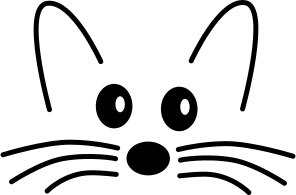
\includegraphics[width=1.4em]{squeak-logo}}}
\newcommand{\dothis}[1]{%
	\medskip
	\noindent\dothisicon
	\ifx#1\empty\else\quad\emph{#1}\fi
	\par\smallskip\nopagebreak}
% NB: To use this in an individual chapter, you must set:
%\graphicspath{{figures/} {../figures/}}
% at the head of the chapter.  Don't forget the final /
%=============================================================
%:Reader hints (hint)
%
% Indicates a non-obvious consequence 
\newcommand{\hint}[1]{\vspace{1ex}\noindent\fbox{\textsc{Astuce}} \emph{#1}}
%=================================================================
% graphics for Morphic handles
\newcommand{\grabHandle}{\raisebox{-0.2ex}{
\includegraphics[width=1em]{blackHandle}}}
\newcommand{\moveHandle}{\raisebox{-0.2ex}{
\includegraphics[width=1em]{moveHandle}}}
\newcommand{\debugHandle}{\raisebox{-0.2ex}{
\includegraphics[width=1em]{debugHandle}}}
% squeak-fr (added for Morphic handles)
\newcommand{\rotateHandle}{\raisebox{-0.2ex}{
\includegraphics[width=1em]{rotateHandle}}}
\newcommand{\viewerHandle}{\raisebox{-0.2ex}{
\includegraphics[width=1em]{viewerHandle}}}
% squeak-fr (add cloverHandle to use \clover in QuickTour.tex as alias
% todo 

%=============================================================
%:Highlighting Important stuff (doublebox)
%
% From Seaside book ...
\newsavebox{\SavedText}
\newlength{\InnerBoxRule}\setlength{\InnerBoxRule}{.75\fboxrule}
\newlength{\OuterBoxRule}\setlength{\OuterBoxRule}{1.5\fboxrule}
\newlength{\BoxSeparation}\setlength{\BoxSeparation}{1.5\fboxrule}
\addtolength{\BoxSeparation}{.5pt}
\newlength{\SaveBoxSep}\setlength{\SaveBoxSep}{2\fboxsep}
%
\newenvironment{doublebox}{\begin{lrbox}{\SavedText}
    \begin{minipage}{.75\textwidth}}
    {\end{minipage}\end{lrbox}\begin{center}
    \setlength{\fboxsep}{\BoxSeparation}\setlength{\fboxrule}{\OuterBoxRule}
    \fbox{\setlength{\fboxsep}{\SaveBoxSep}\setlength{\fboxrule}{\InnerBoxRule}%
      \fbox{\usebox{\SavedText}}}
  \end{center}}
% Use this:
\newcommand{\important}[1]{\begin{doublebox}#1\end{doublebox}}
%=============================================================
%:Section depth
\setcounter{secnumdepth}{2}
%% for this to happen start the file with
%\ifx\wholebook\relax\else
%% $Author$ Martial
% $Date$ Wed Oct 10 13:34:55 CEST 2007
% $Revision$ source: SBE 12715 
% Last Changed Date: 2007-10-08 21:32:45 +0200 (Mon, 08 Oct 2007)
%=============================================================
% NB: documentclass must be set in main document.
% Allows book to be generated in multiple formats.
%=============================================================
%:Packages
\usepackage[french]{babel}
\usepackage[T1]{fontenc}  %%%%%% really important to get the code directly in the text!
\usepackage{lmodern}
%\usepackage[scaled=0.85]{bookmanx} % needs another scale factor if used with \renewcommand{\sfdefault}{cmbr}
\usepackage{palatino}
\usepackage[scaled=0.85]{helvet}
\usepackage{microtype}
\usepackage{graphicx}
\usepackage{theorem}
\usepackage[utf8]{inputenc}
% ON: pdfsync breaks the use of p{width} for tabular columns!
\ifdefined\usepdfsync\usepackage{pdfsync}\fi % Requires texlive 2007
%=============================================================
%:More packages
%Stef should check which ones are used!
%\usepackage{picinpar}
%\usepackage{layout}
%\usepackage{color}
%\usepackage{enum}
%\usepackage{a4wide}
% \usepackage{fancyhdr}
\usepackage{ifthen}
\usepackage{float}
\usepackage{longtable}
\usepackage{makeidx}
\usepackage[nottoc]{tocbibind}
\usepackage{multicol}
\usepackage{booktabs}	% book-style tables
\usepackage{topcapt}	% enables \topcaption
\usepackage{multirow}
\usepackage{tabularx}
%\usepackage[bottom]{footmisc}
\usepackage{xspace}
\usepackage{alltt}
\usepackage{amssymb,textcomp}
\usepackage[usenames,dvipsnames]{color}
%\usepackage{colortbl}
\usepackage[hang]{subfigure}\makeatletter\def\p@subfigure{\thefigure\,}\makeatother
\usepackage{rotating}
\usepackage{enumitem}	% apb: allows more control over tags in enumerations
\usepackage{verbatim}     % for comment environment
\usepackage{varioref}	% for page references that work
\labelformat{footnote}{\thechapter--#1} % to distinguish citations from jurabib
\usepackage{needspace}
\usepackage{isodateo} % enable \isodate
\usepackage[newparttoc]{titlesec}
\usepackage{titletoc}
\usepackage{eurosym}
\usepackage{wrapfig}

\usepackage[
	super,
	citefull=first,
	authorformat={allreversed,and},
	titleformat={commasep,italic}
]{jurabib} % citations as footnotes
\usepackage[
	colorlinks=true,
	linkcolor=black,
	urlcolor=black,
	citecolor=black
]{hyperref}   % should come last

%=============================================================
%:URL style
\makeatletter

\def\url@leostyle{%
  \@ifundefined{selectfont}{\def\UrlFont{\sf}}{\def\UrlFont{\sffamily}}}
% ajouter par Martial pour \traduit (met une dague dans les \doublebox
\def\thempfootnote{\fnsymbol{mpfootnote}}

\makeatother
% Now actually use the newly defined style.
\urlstyle{leo}
%=============================================================
%:Booleans
\newboolean{lulu}
\setboolean{lulu}{false}
\newcommand{\ifluluelse}[2]{\ifthenelse{\boolean{lulu}}{#1}{#2}}
%=============================================================
%:Names
\newcommand{\SUnit}{SUnit\xspace}
\newcommand{\sunit}{SUnit\xspace}
\newcommand{\xUnit}{$x$Unit\xspace}
\newcommand{\JUnit}{JUnit\xspace}
%\newcommand{\XP}{eXtreme Programming\xspace}
\newcommand{\st}{Smalltalk\xspace}
\newcommand{\Squeak}{Squeak\xspace}
\newcommand{\sq}{Squeak\xspace}
\newcommand{\sqmap}{SqueakMap\xspace}
\newcommand{\squeak}{Squeak\xspace}
%\newcommand{\sbe}{\url{scg.unibe.ch/SBE}\xspace}
%\newcommand{\sbe}{\url{squeakbyexample.org}\xspace}
\newcommand{\sbe}{\url{SqueakByExample.org}\xspace}
% squeak-fr: adresse de la version francaise
\newcommand{\spe}{\url{SqueakByExample.org}\xspace} % ?/FR
\newcommand{\sba}{\url{SquareBracketAssociates.org}\xspace}

% squeak-fr: ajout de la \squeakdev pour eviter les problemes de
% changements d'url rencontres dans la VO:
\newcommand{\squeakdev}{\url{www.squeaksource.com/ImageForDevelopers}\xspace} %ou
%\newcommand{\squeakdev}{\url{squeak.ofset.org/squeak-dev}\xspace}

%=============================================================
%:Editorial comment macros
\newcommand{\nnbb}[2]{
    \fbox{\bfseries\sffamily\scriptsize#1}
    {\sf\small$\blacktriangleright$\textit{#2}$\blacktriangleleft$}
   }
\newcommand{\ab}[1]{\nnbb{Andrew}{#1}}
\newcommand{\sd}[1]{\nnbb{St\'{e}f}{#1}}
\newcommand{\md}[1]{\nnbb{Marcus}{#1}}
\newcommand{\on}[1]{\nnbb{Oscar}{#1}}
\newcommand{\damien}[1]{\nnbb{Damien}{#1}}
\newcommand{\lr}[1]{\nnbb{Lukas}{#1}}
\newcommand{\orla}[1]{\nnbb{Orla}{#1}}
%\newcommand{\here}{\nnbb{CONTINUE}{HERE}}
\newcommand{\here}{\nnbb{CONTINUE}{ICI}}

%=============================================================
%:Abbreviation macros
\newcommand{\ie}{\emph{c-\`a-d.}\xspace}
\newcommand{\cad}{\emph{c-\`a-d.}\xspace}
%\newcommand{\eg}{\emph{e.g.},\xspace}
\newcommand{\eg}{\emph{par ex.},\xspace}
\newcommand{\parex}{\emph{par ex.},\xspace}
\newcommand{\etc}{etc\xspace}
%=============================================================
%:Cross reference macros

% [squeak-fr] martial: remarquez les articles devant les noms
\newcommand{\charef}[1]{le chapitre~\ref{cha:#1}\xspace}
% note de martial: utilise dans chapitre Syntax.tex: a redefinir
\newcommand{\charefs}[2]{les chapitres~\ref{cha:#1} et \ref{cha:#2}\xspace}
\newcommand{\secref}[1]{la section~\ref{sec:#1}\xspace}
\newcommand{\figref}[1]{la figure~\ref{fig:#1}\xspace}
\newcommand{\Figref}[1]{La figure~\ref{fig:#1}\xspace}
\newcommand{\appref}[1]{l'annexe~\ref{app:#1}\xspace}
\newcommand{\tabref}[1]{la table~\ref{tab:#1}\xspace}
% defini pour le chapitre Messages.tex
\newcommand{\Tabref}[1]{La table~\ref{tab:#1}\xspace}

% APB: I removed trailing \xspace commands from these macros because
% \xspace mostly doesn't work.  If you want a space after your
% references, type one!
% ON: xspace has always worked just fine for me!  Please leave them in.
%
\newcommand{\ruleref}[1]{\ref{rule:#1}\xspace}
%
\newcommand{\egref}[1]{exemple~\ref{eg:#1}\xspace}
\newcommand{\Egref}[1]{Exemple~\ref{eg:#1}\xspace}
%
\newcommand{\scrref}[1]{script~\ref{scr:#1}\xspace}
\newcommand{\Scrref}[1]{Script~\ref{scr:#1}\xspace}
% t = the
\newcommand{\tscrref}[1]{le script~\ref{scr:#1}\xspace}
\newcommand{\Tscrref}[1]{Le script~\ref{scr:#1}\xspace}
%
\newcommand{\mthref}[1]{m\'ethode~\ref{mth:#1}\xspace}
\newcommand{\mthsref}[1]{m\'ethodes~\ref{mth:#1}\xspace}
\newcommand{\Mthref}[1]{M\'ethode~\ref{mth:#1}\xspace}
\newcommand{\tmthref}[1]{la m\'ethode~\ref{mth:#1}\xspace}
\newcommand{\Tmthref}[1]{La m\'ethode~\ref{mth:#1}\xspace}
%
\newcommand{\clsref}[1]{classe~\ref{cls:#1}\xspace}
\newcommand{\tclsref}[1]{la classe~\ref{cls:#1}\xspace}
\newcommand{\Tclsref}[1]{La classe~\ref{cls:#1}\xspace}
%=============================================================
%:Menu item macro
% for menu items, so we can change our minds on how to print them! (apb)
\definecolor{lightgray}{gray}{0.89}
\newcommand{\menu}[1]{{%
	\setlength{\fboxsep}{0pt}%
	\colorbox{lightgray}{{{\upshape\sffamily\strut \,#1\,}}}}}
% \newcommand{\menu}[1]{{%
% 	\fontfamily{lmr}\selectfont
% 	\upshape\textlangle{\sffamily #1}\textrangle}}
% For submenu items:
\newcommand{\go}{\,$\triangleright$\,}
% \newcommand{\go}{\,$\blacktriangleright$\,}
% For keyboard shortcuts:
%\newcommand{\short}[1]{\mbox{$\langle${\sc CMD}$\rangle$-#1}\xspace}
\newcommand{\short}[1]{\mbox{{\sc cmd}\hspace{0.08em}--\hspace{0.09em}#1}\xspace}
% For buttons:
\newcommand{\button}[1]{{%
	\setlength{\fboxsep}{0pt}%
	\fbox{{\upshape\sffamily\strut \,#1\,}}}}
\newcommand{\toolsflap}{l'onglet \textit{Tools}\xspace}
%=============================================================
%:Reader cues (do this)
%
% Indicate something the reader should try out.
\newcommand{\dothisicon}{\raisebox{-.5ex}{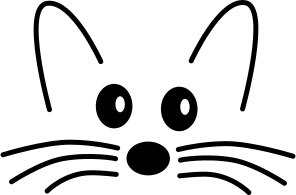
\includegraphics[width=1.4em]{squeak-logo}}}
\newcommand{\dothis}[1]{%
	\medskip
	\noindent\dothisicon
	\ifx#1\empty\else\quad\emph{#1}\fi
	\par\smallskip\nopagebreak}
% NB: To use this in an individual chapter, you must set:
%\graphicspath{{figures/} {../figures/}}
% at the head of the chapter.  Don't forget the final /
%=============================================================
%:Reader hints (hint)
%
% Indicates a non-obvious consequence 
\newcommand{\hint}[1]{\vspace{1ex}\noindent\fbox{\textsc{Astuce}} \emph{#1}}
%=================================================================
% graphics for Morphic handles
\newcommand{\grabHandle}{\raisebox{-0.2ex}{
\includegraphics[width=1em]{blackHandle}}}
\newcommand{\moveHandle}{\raisebox{-0.2ex}{
\includegraphics[width=1em]{moveHandle}}}
\newcommand{\debugHandle}{\raisebox{-0.2ex}{
\includegraphics[width=1em]{debugHandle}}}
% squeak-fr (added for Morphic handles)
\newcommand{\rotateHandle}{\raisebox{-0.2ex}{
\includegraphics[width=1em]{rotateHandle}}}
\newcommand{\viewerHandle}{\raisebox{-0.2ex}{
\includegraphics[width=1em]{viewerHandle}}}
% squeak-fr (add cloverHandle to use \clover in QuickTour.tex as alias
% todo 

%=============================================================
%:Highlighting Important stuff (doublebox)
%
% From Seaside book ...
\newsavebox{\SavedText}
\newlength{\InnerBoxRule}\setlength{\InnerBoxRule}{.75\fboxrule}
\newlength{\OuterBoxRule}\setlength{\OuterBoxRule}{1.5\fboxrule}
\newlength{\BoxSeparation}\setlength{\BoxSeparation}{1.5\fboxrule}
\addtolength{\BoxSeparation}{.5pt}
\newlength{\SaveBoxSep}\setlength{\SaveBoxSep}{2\fboxsep}
%
\newenvironment{doublebox}{\begin{lrbox}{\SavedText}
    \begin{minipage}{.75\textwidth}}
    {\end{minipage}\end{lrbox}\begin{center}
    \setlength{\fboxsep}{\BoxSeparation}\setlength{\fboxrule}{\OuterBoxRule}
    \fbox{\setlength{\fboxsep}{\SaveBoxSep}\setlength{\fboxrule}{\InnerBoxRule}%
      \fbox{\usebox{\SavedText}}}
  \end{center}}
% Use this:
\newcommand{\important}[1]{\begin{doublebox}#1\end{doublebox}}
%=============================================================
%:Section depth
\setcounter{secnumdepth}{2}
%% for this to happen start the file with
%\ifx\wholebook\relax\else
%% $Author$ Martial
% $Date$ Wed Oct 10 13:34:55 CEST 2007
% $Revision$ source: SBE 12715 
% Last Changed Date: 2007-10-08 21:32:45 +0200 (Mon, 08 Oct 2007)
%=============================================================
% NB: documentclass must be set in main document.
% Allows book to be generated in multiple formats.
%=============================================================
%:Packages
\usepackage[french]{babel}
\usepackage[T1]{fontenc}  %%%%%% really important to get the code directly in the text!
\usepackage{lmodern}
%\usepackage[scaled=0.85]{bookmanx} % needs another scale factor if used with \renewcommand{\sfdefault}{cmbr}
\usepackage{palatino}
\usepackage[scaled=0.85]{helvet}
\usepackage{microtype}
\usepackage{graphicx}
\usepackage{theorem}
\usepackage[utf8]{inputenc}
% ON: pdfsync breaks the use of p{width} for tabular columns!
\ifdefined\usepdfsync\usepackage{pdfsync}\fi % Requires texlive 2007
%=============================================================
%:More packages
%Stef should check which ones are used!
%\usepackage{picinpar}
%\usepackage{layout}
%\usepackage{color}
%\usepackage{enum}
%\usepackage{a4wide}
% \usepackage{fancyhdr}
\usepackage{ifthen}
\usepackage{float}
\usepackage{longtable}
\usepackage{makeidx}
\usepackage[nottoc]{tocbibind}
\usepackage{multicol}
\usepackage{booktabs}	% book-style tables
\usepackage{topcapt}	% enables \topcaption
\usepackage{multirow}
\usepackage{tabularx}
%\usepackage[bottom]{footmisc}
\usepackage{xspace}
\usepackage{alltt}
\usepackage{amssymb,textcomp}
\usepackage[usenames,dvipsnames]{color}
%\usepackage{colortbl}
\usepackage[hang]{subfigure}\makeatletter\def\p@subfigure{\thefigure\,}\makeatother
\usepackage{rotating}
\usepackage{enumitem}	% apb: allows more control over tags in enumerations
\usepackage{verbatim}     % for comment environment
\usepackage{varioref}	% for page references that work
\labelformat{footnote}{\thechapter--#1} % to distinguish citations from jurabib
\usepackage{needspace}
\usepackage{isodateo} % enable \isodate
\usepackage[newparttoc]{titlesec}
\usepackage{titletoc}
\usepackage{eurosym}
\usepackage{wrapfig}

\usepackage[
	super,
	citefull=first,
	authorformat={allreversed,and},
	titleformat={commasep,italic}
]{jurabib} % citations as footnotes
\usepackage[
	colorlinks=true,
	linkcolor=black,
	urlcolor=black,
	citecolor=black
]{hyperref}   % should come last

%=============================================================
%:URL style
\makeatletter

\def\url@leostyle{%
  \@ifundefined{selectfont}{\def\UrlFont{\sf}}{\def\UrlFont{\sffamily}}}
% ajouter par Martial pour \traduit (met une dague dans les \doublebox
\def\thempfootnote{\fnsymbol{mpfootnote}}

\makeatother
% Now actually use the newly defined style.
\urlstyle{leo}
%=============================================================
%:Booleans
\newboolean{lulu}
\setboolean{lulu}{false}
\newcommand{\ifluluelse}[2]{\ifthenelse{\boolean{lulu}}{#1}{#2}}
%=============================================================
%:Names
\newcommand{\SUnit}{SUnit\xspace}
\newcommand{\sunit}{SUnit\xspace}
\newcommand{\xUnit}{$x$Unit\xspace}
\newcommand{\JUnit}{JUnit\xspace}
%\newcommand{\XP}{eXtreme Programming\xspace}
\newcommand{\st}{Smalltalk\xspace}
\newcommand{\Squeak}{Squeak\xspace}
\newcommand{\sq}{Squeak\xspace}
\newcommand{\sqmap}{SqueakMap\xspace}
\newcommand{\squeak}{Squeak\xspace}
%\newcommand{\sbe}{\url{scg.unibe.ch/SBE}\xspace}
%\newcommand{\sbe}{\url{squeakbyexample.org}\xspace}
\newcommand{\sbe}{\url{SqueakByExample.org}\xspace}
% squeak-fr: adresse de la version francaise
\newcommand{\spe}{\url{SqueakByExample.org}\xspace} % ?/FR
\newcommand{\sba}{\url{SquareBracketAssociates.org}\xspace}

% squeak-fr: ajout de la \squeakdev pour eviter les problemes de
% changements d'url rencontres dans la VO:
\newcommand{\squeakdev}{\url{www.squeaksource.com/ImageForDevelopers}\xspace} %ou
%\newcommand{\squeakdev}{\url{squeak.ofset.org/squeak-dev}\xspace}

%=============================================================
%:Editorial comment macros
\newcommand{\nnbb}[2]{
    \fbox{\bfseries\sffamily\scriptsize#1}
    {\sf\small$\blacktriangleright$\textit{#2}$\blacktriangleleft$}
   }
\newcommand{\ab}[1]{\nnbb{Andrew}{#1}}
\newcommand{\sd}[1]{\nnbb{St\'{e}f}{#1}}
\newcommand{\md}[1]{\nnbb{Marcus}{#1}}
\newcommand{\on}[1]{\nnbb{Oscar}{#1}}
\newcommand{\damien}[1]{\nnbb{Damien}{#1}}
\newcommand{\lr}[1]{\nnbb{Lukas}{#1}}
\newcommand{\orla}[1]{\nnbb{Orla}{#1}}
%\newcommand{\here}{\nnbb{CONTINUE}{HERE}}
\newcommand{\here}{\nnbb{CONTINUE}{ICI}}

%=============================================================
%:Abbreviation macros
\newcommand{\ie}{\emph{c-\`a-d.}\xspace}
\newcommand{\cad}{\emph{c-\`a-d.}\xspace}
%\newcommand{\eg}{\emph{e.g.},\xspace}
\newcommand{\eg}{\emph{par ex.},\xspace}
\newcommand{\parex}{\emph{par ex.},\xspace}
\newcommand{\etc}{etc\xspace}
%=============================================================
%:Cross reference macros

% [squeak-fr] martial: remarquez les articles devant les noms
\newcommand{\charef}[1]{le chapitre~\ref{cha:#1}\xspace}
% note de martial: utilise dans chapitre Syntax.tex: a redefinir
\newcommand{\charefs}[2]{les chapitres~\ref{cha:#1} et \ref{cha:#2}\xspace}
\newcommand{\secref}[1]{la section~\ref{sec:#1}\xspace}
\newcommand{\figref}[1]{la figure~\ref{fig:#1}\xspace}
\newcommand{\Figref}[1]{La figure~\ref{fig:#1}\xspace}
\newcommand{\appref}[1]{l'annexe~\ref{app:#1}\xspace}
\newcommand{\tabref}[1]{la table~\ref{tab:#1}\xspace}
% defini pour le chapitre Messages.tex
\newcommand{\Tabref}[1]{La table~\ref{tab:#1}\xspace}

% APB: I removed trailing \xspace commands from these macros because
% \xspace mostly doesn't work.  If you want a space after your
% references, type one!
% ON: xspace has always worked just fine for me!  Please leave them in.
%
\newcommand{\ruleref}[1]{\ref{rule:#1}\xspace}
%
\newcommand{\egref}[1]{exemple~\ref{eg:#1}\xspace}
\newcommand{\Egref}[1]{Exemple~\ref{eg:#1}\xspace}
%
\newcommand{\scrref}[1]{script~\ref{scr:#1}\xspace}
\newcommand{\Scrref}[1]{Script~\ref{scr:#1}\xspace}
% t = the
\newcommand{\tscrref}[1]{le script~\ref{scr:#1}\xspace}
\newcommand{\Tscrref}[1]{Le script~\ref{scr:#1}\xspace}
%
\newcommand{\mthref}[1]{m\'ethode~\ref{mth:#1}\xspace}
\newcommand{\mthsref}[1]{m\'ethodes~\ref{mth:#1}\xspace}
\newcommand{\Mthref}[1]{M\'ethode~\ref{mth:#1}\xspace}
\newcommand{\tmthref}[1]{la m\'ethode~\ref{mth:#1}\xspace}
\newcommand{\Tmthref}[1]{La m\'ethode~\ref{mth:#1}\xspace}
%
\newcommand{\clsref}[1]{classe~\ref{cls:#1}\xspace}
\newcommand{\tclsref}[1]{la classe~\ref{cls:#1}\xspace}
\newcommand{\Tclsref}[1]{La classe~\ref{cls:#1}\xspace}
%=============================================================
%:Menu item macro
% for menu items, so we can change our minds on how to print them! (apb)
\definecolor{lightgray}{gray}{0.89}
\newcommand{\menu}[1]{{%
	\setlength{\fboxsep}{0pt}%
	\colorbox{lightgray}{{{\upshape\sffamily\strut \,#1\,}}}}}
% \newcommand{\menu}[1]{{%
% 	\fontfamily{lmr}\selectfont
% 	\upshape\textlangle{\sffamily #1}\textrangle}}
% For submenu items:
\newcommand{\go}{\,$\triangleright$\,}
% \newcommand{\go}{\,$\blacktriangleright$\,}
% For keyboard shortcuts:
%\newcommand{\short}[1]{\mbox{$\langle${\sc CMD}$\rangle$-#1}\xspace}
\newcommand{\short}[1]{\mbox{{\sc cmd}\hspace{0.08em}--\hspace{0.09em}#1}\xspace}
% For buttons:
\newcommand{\button}[1]{{%
	\setlength{\fboxsep}{0pt}%
	\fbox{{\upshape\sffamily\strut \,#1\,}}}}
\newcommand{\toolsflap}{l'onglet \textit{Tools}\xspace}
%=============================================================
%:Reader cues (do this)
%
% Indicate something the reader should try out.
\newcommand{\dothisicon}{\raisebox{-.5ex}{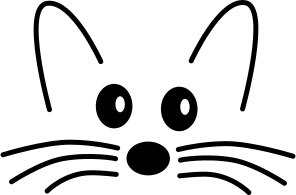
\includegraphics[width=1.4em]{squeak-logo}}}
\newcommand{\dothis}[1]{%
	\medskip
	\noindent\dothisicon
	\ifx#1\empty\else\quad\emph{#1}\fi
	\par\smallskip\nopagebreak}
% NB: To use this in an individual chapter, you must set:
%\graphicspath{{figures/} {../figures/}}
% at the head of the chapter.  Don't forget the final /
%=============================================================
%:Reader hints (hint)
%
% Indicates a non-obvious consequence 
\newcommand{\hint}[1]{\vspace{1ex}\noindent\fbox{\textsc{Astuce}} \emph{#1}}
%=================================================================
% graphics for Morphic handles
\newcommand{\grabHandle}{\raisebox{-0.2ex}{
\includegraphics[width=1em]{blackHandle}}}
\newcommand{\moveHandle}{\raisebox{-0.2ex}{
\includegraphics[width=1em]{moveHandle}}}
\newcommand{\debugHandle}{\raisebox{-0.2ex}{
\includegraphics[width=1em]{debugHandle}}}
% squeak-fr (added for Morphic handles)
\newcommand{\rotateHandle}{\raisebox{-0.2ex}{
\includegraphics[width=1em]{rotateHandle}}}
\newcommand{\viewerHandle}{\raisebox{-0.2ex}{
\includegraphics[width=1em]{viewerHandle}}}
% squeak-fr (add cloverHandle to use \clover in QuickTour.tex as alias
% todo 

%=============================================================
%:Highlighting Important stuff (doublebox)
%
% From Seaside book ...
\newsavebox{\SavedText}
\newlength{\InnerBoxRule}\setlength{\InnerBoxRule}{.75\fboxrule}
\newlength{\OuterBoxRule}\setlength{\OuterBoxRule}{1.5\fboxrule}
\newlength{\BoxSeparation}\setlength{\BoxSeparation}{1.5\fboxrule}
\addtolength{\BoxSeparation}{.5pt}
\newlength{\SaveBoxSep}\setlength{\SaveBoxSep}{2\fboxsep}
%
\newenvironment{doublebox}{\begin{lrbox}{\SavedText}
    \begin{minipage}{.75\textwidth}}
    {\end{minipage}\end{lrbox}\begin{center}
    \setlength{\fboxsep}{\BoxSeparation}\setlength{\fboxrule}{\OuterBoxRule}
    \fbox{\setlength{\fboxsep}{\SaveBoxSep}\setlength{\fboxrule}{\InnerBoxRule}%
      \fbox{\usebox{\SavedText}}}
  \end{center}}
% Use this:
\newcommand{\important}[1]{\begin{doublebox}#1\end{doublebox}}
%=============================================================
%:Section depth
\setcounter{secnumdepth}{2}
%% for this to happen start the file with
%\ifx\wholebook\relax\else
%\input{../common.tex}
%\begin{document}
%\fi
% and terminate by
% \ifx\wholebook\relax\else\end{document}\fi

\DeclareGraphicsExtensions{.pdf, .jpg, .png}
%=============================================================
%:PDF setup
\hypersetup{
%   a4paper,
%   pdfstartview=FitV,
%   colorlinks,
%   linkcolor=darkblue,
%   citecolor=darkblue,
%   pdftitle={Squeak by Example},
pdftitle={Squeak par l'exemple},
   pdfauthor={Andrew Black, St\'ephane Ducasse,	Oscar Nierstrasz,
Damien Pollet},
   pdfkeywords={Smalltalk, Squeak, Programmation Orient\'ee Objet},
pdfsubject={Informatique, Computer Science}
}
%=============================================================
%:Page layout and appearance
%
% \renewcommand{\headrulewidth}{0pt}
\renewcommand{\chaptermark}[1]{\markboth{#1}{}}
\renewcommand{\sectionmark}[1]{\markright{\thesection\ #1}}
\renewpagestyle{plain}[\small\itshape]{%
	\setheadrule{0pt}%
	\sethead[\thepage][][]{}{}{\thepage}%
	\setfoot[][][]{}{}{}}
\renewpagestyle{headings}[\small\itshape]{%
	\setheadrule{0pt}%
	\setmarks{chapter}{section}%
	\sethead[\thepage][][\chaptertitle]{\sectiontitle}{}{\thepage}%
	\setfoot[][][]{}{}{}}
%=============================================================
%:Title section setup and TOC numbering depth
\setcounter{secnumdepth}{1}
\setcounter{tocdepth}{1}
\titleformat{\part}[display]{\centering}{\huge\partname\ \thepart}{1em}{\Huge\textbf}[]
\titleformat{\chapter}[display]{}{\huge\chaptertitlename\ \thechapter}{1em}{\Huge\raggedright\textbf}[]
\titlecontents{part}[3pc]{%
		\pagebreak[2]\addvspace{1em plus.4em minus.2em}%
		\leavevmode\large\bfseries}
	{\contentslabel{3pc}}{\hspace*{-3pc}}
	{}[\nopagebreak]
\titlecontents{chapter}[3pc]{%
		\pagebreak[0]\addvspace{1em plus.2em minus.2em}%
		\leavevmode\bfseries}
	{\contentslabel{3pc}}{}
	{\hfill\contentspage}[\nopagebreak]
\dottedcontents{section}[3pc]{}{3pc}{1pc}
\dottedcontents{subsection}[3pc]{}{0pc}{1pc}
% \dottedcontents{subsection}[4.5em]{}{0pt}{1pc}
% Make \cleardoublepage insert really blank pages http://www.tex.ac.uk/cgi-bin/texfaq2html?label=reallyblank
\let\origdoublepage\cleardoublepage
\newcommand{\clearemptydoublepage}{%
  \clearpage
  {\pagestyle{empty}\origdoublepage}}
\let\cleardoublepage\clearemptydoublepage % see http://www.tex.ac.uk/cgi-bin/texfaq2html?label=patch
%=============================================================
%:FAQ macros (for FAQ chapter)
\newtheorem{faq}{FAQ}
\newcommand{\answer}{\paragraph{R\'eponse}\ }
%=============================================================
%:Listings package configuration
\usepackage{listings}
\newcommand{\caret}{\makebox{\raisebox{0.4ex}{\footnotesize{$\wedge$}}}}
\lstdefinelanguage{Smalltalk}{
%  morekeywords={self,super,true,false,nil,thisContext}, % This is overkill
  morestring=[d]',
  morecomment=[s]{"}{"},
  alsoletter={\#:},
  escapechar={!},
  escapebegin=\itshape, % comment-like by default (Martial 11/2007)
  literate=
    {BANG}{!}1
    {UNDERSCORE}{\_}1
    {\\st}{Smalltalk}9 % convenience -- in case \st occurs in code
    % {'}{{\textquotesingle}}1 % replaced by upquote=true in \lstset
    {_}{{$\leftarrow$}}1
    {>>>}{{\sep}}1
    {^}{{$\uparrow$}}1
    {~}{{$\sim$}}1
    {-}{{\sf -\hspace{-0.13em}-}}1  % the goal is to make - the same width as +
    {+}{\raisebox{0.08ex}{+}}1		% and to raise + off the baseline to match -
    {-->}{{\quad$\longrightarrow$\quad}}3
	, % Don't forget the comma at the end!
  tabsize=4
}[keywords,comments,strings]
% ajout pour les échappements dans les codes
% indispensable pour mettre le code en emphase (cf. Model.tex) 
\newcommand{\codeify}[1]{\NoAutoSpaceBeforeFDP#1\AutoSpaceBeforeFDP}
\newcommand{\normcomment}[1]{\emph{#1}} %cf. Streams
\newcommand{\normcode}[1]{\emph{\codeify{#1}}} %cf. Streams
\newcommand{\emcode}[1]{\textbf{\normcode{#1}}} % Martial 11/2007
\lstset{language=Smalltalk,
	basicstyle=\sffamily,
	keywordstyle=\color{black}\bfseries,
	% stringstyle=\ttfamily, % Ugly! do we really want this? -- on
	%commentstyle=\itshape,
	mathescape=true,
	showstringspaces=false,
	keepspaces=true,
	breaklines=true,
	breakautoindent=true,
	lineskip={-1pt}, % Ugly hack
	upquote=true, % straight quote; requires textcomp package
	columns=fullflexible} % no fixed width fonts
% In-line code (literal)
% Normally use this for all in-line code:
\newcommand{\ct}{\lstinline[mathescape=false,basicstyle={\sffamily\upshape}]}
% apb 2007.8.28 added the \upshape declaration to avoid getting italicized code in \dothis{ } sections.
% In-line code (latex enabled)
% Use this only in special situations where \ct does not work
% (within section headings ...):

% [squeak-fr] Modification de \lct suivant les indications de Martial Boniou
\newcommand{\lct}[1]{\textsf{\textup{\NoAutoSpaceBeforeFDP #1
\AutoSpaceBeforeFDP}}} %\xspace

% Use these for system categories and protocols:
\newcommand{\scat}[1]{\emph{\textsf{#1}}\xspace}
\newcommand{\pkg}[1]{\emph{\textsf{#1}}\xspace}
\newcommand{\prot}[1]{\emph{\textsf{#1}}\xspace}
% Code environments
% NB: the arg is for tests
% Only code and example environments may be tests
\lstnewenvironment{code}[1]{%
	\lstset{%
		frame=lines,
		mathescape=false
	}
}{}
\def\ignoredollar#1{}
%=============================================================
%:Code environments (method, script ...)
% NB: the third arg is for tests
% Only code and example environments may be tests
\lstnewenvironment{example}[3][defaultlabel]{%
	\renewcommand{\lstlistingname}{Exemple}%
	\lstset{
		frame=lines,
		mathescape=false,
		caption={\emph{#2}},
		label={eg:#1}
	}
}{}
\lstnewenvironment{script}[2][defaultlabel]{%
\renewcommand{\lstlistingname}{Script}%
	\lstset{
		frame=lines,
		mathescape=false,
		name={Script},
		caption={\emph{#2}},
		label={scr:#1}
	}
}{}
\lstnewenvironment{method}[2][defaultlabel]{%
	\renewcommand{\lstlistingname}{M\'ethode}%
	\lstset{
		frame=lines,
		mathescape=false,
		name={M\'ethode},
		caption={\emph{#2}},
		label={mth:#1}
	}
}{}
\lstnewenvironment{methods}[2][defaultlabel]{% just for multiple methods at once
	\renewcommand{\lstlistingname}{M\'ethodes}%
	\lstset{
		frame=lines,
		mathescape=false,
		name={M\'ethode},
		caption={\emph{#2}},
		label={mth:#1}
	}
}{}
\lstnewenvironment{numMethod}[2][defaultlabel]{%
	\renewcommand{\lstlistingname}{M\'ethode}%
	\lstset{
		numbers=left,
		numberstyle={\tiny\sffamily},
		frame=lines,
		mathescape=false,
		name={M\'ethode},
		caption={\emph{#2}},
		label={mth:#1}
	}
}{}
\lstnewenvironment{classdef}[2][defaultlabel]{%
	\renewcommand{\lstlistingname}{Classe}%
	\lstset{
		frame=lines,
		mathescape=false,
		name={Classe},
		caption={\emph{#2}},
		label={cls:#1}
	}
}{}
%=============================================================
%:Reserving space
% Usually need one more line than the actual lines of code
\newcommand{\needlines}[1]{\Needspace{#1\baselineskip}}
%=============================================================
%:Indexing macros
% Macros ending with "ind" generate text as well as an index entry
% Macros ending with "index" *only* generate an index entry
\newcommand{\ind}[1]{\index{#1}#1\xspace} % plain text
\newcommand{\subind}[2]{\index{#1!#2}#2\xspace} % show #2, subindex inder #1
\newcommand{\emphind}[1]{\index{#1}\emph{#1}\xspace} % emph #1
\newcommand{\emphsubind}[2]{\index{#1!#2}\emph{#2}\xspace} % show emph #2, subindex inder #1
\newcommand{\scatind}[1]{\index{#1@\textsf{#1} (cat\'egorie)}\scat{#1}} % category
\newcommand{\protind}[1]{\index{#1@\textsf{#1} (protocole)}\prot{#1}} % protocol
% \newcommand{\clsind}[1]{\index{#1@\textsf{#1} (class)}\ct{#1}\xspace}
\newcommand{\clsind}[1]{\index{#1!\#@(classe)}\ct{#1}\xspace} % class
\newcommand{\cvind}[1]{\index{#1@\textsf{#1} (variable de classe)}\ct{#1}\xspace} % class var
\newcommand{\glbind}[1]{\index{#1@\textsf{#1} (globale)}\ct{#1}\xspace} % global
\newcommand{\patind}[1]{\index{#1@#1 (patron)}\ct{#1}\xspace} % pattern
\newcommand{\pvind}[1]{\index{#1@\textsf{#1} (pseudo-variable)}\ct{#1}\xspace} % pseudo variable
% [squeak - fr]Martial: I found the following cleaner (should be
% merged in SBE for self and super)
\newcommand{\subpvindex}[2]{\index{#1@\textsf{#1} (pseudo-variable)!#2}}
\newcommand{\subpvind}[2]{\index{#1@\textsf{#1} (pseudo-variable)!#2}#2\xspace}
% used in Model.tex
\newcommand{\mthind}[2]{\index{#1!#2@\ct{#2}}\ct{#2}\xspace} % show method name only
\newcommand{\lmthind}[2]{\index{#1!#2@\ct{#2}}\lct{#2}\xspace} % show method name only
\newcommand{\cmind}[2]{\index{#1!#2@\ct{#2}}\ct{#1>>>#2}\xspace} % show class>>method
\newcommand{\toolsflapind}{\index{onglet Tools}\toolsflap} % index tools flap
% The following only generate an index entry:
% \newcommand{\clsindex}[1]{\index{#1@\textsf{#1} (class)}}
\newcommand{\clsindex}[1]{\index{#1!\#@(classe)}} % class
\newcommand{\cmindex}[2]{\index{#1!#2@\ct{#2}}} % class>>method
\newcommand{\cvindex}[1]{\index{#1@\textsf{#1} (variable de classe)}} % class var
\newcommand{\glbindex}[1]{\index{#1@\textsf{#1} (globale)}}% global
\newcommand{\pvindex}[1]{\index{#1@\textsf{#1} (pseudo-variable)}}% pseudo var
\newcommand{\seeindex}[2]{\index{#1|see{#2}}} % #1, see #2
\newcommand{\scatindex}[1]{\index{#1@\textsf{#1} (cat\'egorie)}} % category
\newcommand{\protindex}[1]{\index{#1@\textsf{#1} (protocole)}} % protocol
% How can we have the main entry page numbers in bold yet not break the hyperlink?
\newcommand{\boldidx}[1]{{\bf #1}} % breaks hyperlink
%\newcommand{\indmain}[1]{\index{#1|boldidx}#1\xspace} % plain text, main entry
%\newcommand{\emphsubindmain}[2]{\index{#1!#2|boldidx}\emph{#2}\xspace} % subindex, main entry
%\newcommand{\subindmain}[2]{\index{#1!#2|boldidx}#2\xspace} % subindex, main entry
%\newcommand{\clsindmain}[1]{\index{#1@\textsf{#1} (class)|boldidx}\ct{#1}\xspace}
%\newcommand{\clsindmain}[1]{\index{#1!\#@(class)|boldidx}\ct{#1}\xspace} % class main
%\newcommand{\indexmain}[1]{\index{#1|boldidx}} % main index entry only
\newcommand{\indmain}[1]{\index{#1}#1\xspace} 
\newcommand{\emphsubindmain}[2]{\index{#1!#2}\emph{#2}\xspace} % subindex, main entry
\newcommand{\subindmain}[2]{\index{#1!#2}#2\xspace} % subindex, main entry
%\newcommand{\clsindmain}[1]{\index{#1@\textsf{#1} (class)}\ct{#1}\xspace}
\newcommand{\clsindmain}[1]{\index{#1!\#@(classe)}\ct{#1}\xspace} % class main
\newcommand{\indexmain}[1]{\index{#1}} 
%=============================================================
%:Code macros
% some constants
\newcommand{\codesize}{\small}
\newcommand{\codefont}{\sffamily}
\newcommand{\cat}[1]{\textit{Dans la cat\'egorie #1}}%%To remove later
\newlength{\scriptindent}
\setlength{\scriptindent}{.3cm}
%% Method presentation constants
\newlength{\methodindent}
\newlength{\methodwordlength}
\newlength{\aftermethod}
\setlength{\methodindent}{0.2cm}
\settowidth{\methodwordlength}{\ M\'ethode\ }
%=============================================================
%:Smalltalk macros
%\newcommand{\sep}{{$\gg$}}
\newcommand{\sep}{\mbox{>>}}
\newcommand{\self}{\ct{self}\xspace}
\newcommand{\super}{\ct{super}\xspace}
\newcommand{\nil}{\ct{nil}\xspace}
%=============================================================
% be less conservative about float placement
% these commands are from http://www.tex.ac.uk/cgi-bin/texfaq2html?label=floats
\renewcommand{\topfraction}{.9}
\renewcommand{\bottomfraction}{.9}
\renewcommand{\textfraction}{.1}
\renewcommand{\floatpagefraction}{.85}
\renewcommand{\dbltopfraction}{.66}
\renewcommand{\dblfloatpagefraction}{.85}
\setcounter{topnumber}{9}
\setcounter{bottomnumber}{9}
\setcounter{totalnumber}{20}
\setcounter{dbltopnumber}{9}
%=============================================================
%% [Squeak-fr]
% pour identifier les zones de texte à corriger d'urgence!
\newcommand{\arevoir}[1]{#1}
% \traduit utilisé dans Model.tex
\newcommand{\traduit}[1]{\footnote[2]{#1}}
% changeset alias
\newcommand{\changeset}{\emph{change set}\xspace}
\newcommand{\changesets}{\emph{change sets}\xspace}
% callback alias
\newcommand{\callback}{\emph{callback}\xspace}
% blobmorph alias (QuickTour->blob)
\newcommand{\blobmorph}{\emph{blob}\xspace}
% repository
\newcommand{\squeaksource}{\textsf{SqueakSource}\xspace}
\newcommand{\sourceforge}{\textsf{SourceForge}\xspace}
% L'onglet Tools
\newcommand{\Toolsflap}{L'onglet \textit{Tools}\xspace}
% Mac OS X
\newcommand{\macosx}{\mbox{Mac OS X}\xspace}
% code en francais (uniquement dans le chapitre BasicClasses)
\newcommand{\codefrench}[1]{\NoAutoSpaceBeforeFDP\texttt{#1}\AutoSpaceBeforeFDP\xspace}
% mantra du modele objet (suite a l'erreur de martial)
\newcommand{\Mantra}{Tout est objet\xspace}
\newcommand{\mantra}{\MakeLowercase{\Mantra}\xspace}
% césure
\hyphenation{Omni-Brow-ser}
\hyphenation{m\'e-tho-de} % erreur de cesure commune
\hyphenation{m\'e-tho-des}
\hyphenation{e-xem-ple}
\hyphenation{en-re-gi-stre}
\hyphenation{a-na-ly-seur}
\hyphenation{glo-ba-le}
\hyphenation{fi-gu-re}
\hyphenation{vi-si-bles}
\hyphenation{cor-res-pon-dan-te}
\hyphenation{Work-space}
%=============================================================
% apb doesn't like paragraphs to run in to each other without a break
\parskip 1ex
%=============================================================
%:Stuff to check, merge or deprecate
%\setlength{\marginparsep}{2mm}
%\renewcommand{\baselinestretch}{1.1}
%=============================================================

%\begin{document}
%\fi
% and terminate by
% \ifx\wholebook\relax\else\end{document}\fi

\DeclareGraphicsExtensions{.pdf, .jpg, .png}
%=============================================================
%:PDF setup
\hypersetup{
%   a4paper,
%   pdfstartview=FitV,
%   colorlinks,
%   linkcolor=darkblue,
%   citecolor=darkblue,
%   pdftitle={Squeak by Example},
pdftitle={Squeak par l'exemple},
   pdfauthor={Andrew Black, St\'ephane Ducasse,	Oscar Nierstrasz,
Damien Pollet},
   pdfkeywords={Smalltalk, Squeak, Programmation Orient\'ee Objet},
pdfsubject={Informatique, Computer Science}
}
%=============================================================
%:Page layout and appearance
%
% \renewcommand{\headrulewidth}{0pt}
\renewcommand{\chaptermark}[1]{\markboth{#1}{}}
\renewcommand{\sectionmark}[1]{\markright{\thesection\ #1}}
\renewpagestyle{plain}[\small\itshape]{%
	\setheadrule{0pt}%
	\sethead[\thepage][][]{}{}{\thepage}%
	\setfoot[][][]{}{}{}}
\renewpagestyle{headings}[\small\itshape]{%
	\setheadrule{0pt}%
	\setmarks{chapter}{section}%
	\sethead[\thepage][][\chaptertitle]{\sectiontitle}{}{\thepage}%
	\setfoot[][][]{}{}{}}
%=============================================================
%:Title section setup and TOC numbering depth
\setcounter{secnumdepth}{1}
\setcounter{tocdepth}{1}
\titleformat{\part}[display]{\centering}{\huge\partname\ \thepart}{1em}{\Huge\textbf}[]
\titleformat{\chapter}[display]{}{\huge\chaptertitlename\ \thechapter}{1em}{\Huge\raggedright\textbf}[]
\titlecontents{part}[3pc]{%
		\pagebreak[2]\addvspace{1em plus.4em minus.2em}%
		\leavevmode\large\bfseries}
	{\contentslabel{3pc}}{\hspace*{-3pc}}
	{}[\nopagebreak]
\titlecontents{chapter}[3pc]{%
		\pagebreak[0]\addvspace{1em plus.2em minus.2em}%
		\leavevmode\bfseries}
	{\contentslabel{3pc}}{}
	{\hfill\contentspage}[\nopagebreak]
\dottedcontents{section}[3pc]{}{3pc}{1pc}
\dottedcontents{subsection}[3pc]{}{0pc}{1pc}
% \dottedcontents{subsection}[4.5em]{}{0pt}{1pc}
% Make \cleardoublepage insert really blank pages http://www.tex.ac.uk/cgi-bin/texfaq2html?label=reallyblank
\let\origdoublepage\cleardoublepage
\newcommand{\clearemptydoublepage}{%
  \clearpage
  {\pagestyle{empty}\origdoublepage}}
\let\cleardoublepage\clearemptydoublepage % see http://www.tex.ac.uk/cgi-bin/texfaq2html?label=patch
%=============================================================
%:FAQ macros (for FAQ chapter)
\newtheorem{faq}{FAQ}
\newcommand{\answer}{\paragraph{R\'eponse}\ }
%=============================================================
%:Listings package configuration
\usepackage{listings}
\newcommand{\caret}{\makebox{\raisebox{0.4ex}{\footnotesize{$\wedge$}}}}
\lstdefinelanguage{Smalltalk}{
%  morekeywords={self,super,true,false,nil,thisContext}, % This is overkill
  morestring=[d]',
  morecomment=[s]{"}{"},
  alsoletter={\#:},
  escapechar={!},
  escapebegin=\itshape, % comment-like by default (Martial 11/2007)
  literate=
    {BANG}{!}1
    {UNDERSCORE}{\_}1
    {\\st}{Smalltalk}9 % convenience -- in case \st occurs in code
    % {'}{{\textquotesingle}}1 % replaced by upquote=true in \lstset
    {_}{{$\leftarrow$}}1
    {>>>}{{\sep}}1
    {^}{{$\uparrow$}}1
    {~}{{$\sim$}}1
    {-}{{\sf -\hspace{-0.13em}-}}1  % the goal is to make - the same width as +
    {+}{\raisebox{0.08ex}{+}}1		% and to raise + off the baseline to match -
    {-->}{{\quad$\longrightarrow$\quad}}3
	, % Don't forget the comma at the end!
  tabsize=4
}[keywords,comments,strings]
% ajout pour les échappements dans les codes
% indispensable pour mettre le code en emphase (cf. Model.tex) 
\newcommand{\codeify}[1]{\NoAutoSpaceBeforeFDP#1\AutoSpaceBeforeFDP}
\newcommand{\normcomment}[1]{\emph{#1}} %cf. Streams
\newcommand{\normcode}[1]{\emph{\codeify{#1}}} %cf. Streams
\newcommand{\emcode}[1]{\textbf{\normcode{#1}}} % Martial 11/2007
\lstset{language=Smalltalk,
	basicstyle=\sffamily,
	keywordstyle=\color{black}\bfseries,
	% stringstyle=\ttfamily, % Ugly! do we really want this? -- on
	%commentstyle=\itshape,
	mathescape=true,
	showstringspaces=false,
	keepspaces=true,
	breaklines=true,
	breakautoindent=true,
	lineskip={-1pt}, % Ugly hack
	upquote=true, % straight quote; requires textcomp package
	columns=fullflexible} % no fixed width fonts
% In-line code (literal)
% Normally use this for all in-line code:
\newcommand{\ct}{\lstinline[mathescape=false,basicstyle={\sffamily\upshape}]}
% apb 2007.8.28 added the \upshape declaration to avoid getting italicized code in \dothis{ } sections.
% In-line code (latex enabled)
% Use this only in special situations where \ct does not work
% (within section headings ...):

% [squeak-fr] Modification de \lct suivant les indications de Martial Boniou
\newcommand{\lct}[1]{\textsf{\textup{\NoAutoSpaceBeforeFDP #1
\AutoSpaceBeforeFDP}}} %\xspace

% Use these for system categories and protocols:
\newcommand{\scat}[1]{\emph{\textsf{#1}}\xspace}
\newcommand{\pkg}[1]{\emph{\textsf{#1}}\xspace}
\newcommand{\prot}[1]{\emph{\textsf{#1}}\xspace}
% Code environments
% NB: the arg is for tests
% Only code and example environments may be tests
\lstnewenvironment{code}[1]{%
	\lstset{%
		frame=lines,
		mathescape=false
	}
}{}
\def\ignoredollar#1{}
%=============================================================
%:Code environments (method, script ...)
% NB: the third arg is for tests
% Only code and example environments may be tests
\lstnewenvironment{example}[3][defaultlabel]{%
	\renewcommand{\lstlistingname}{Exemple}%
	\lstset{
		frame=lines,
		mathescape=false,
		caption={\emph{#2}},
		label={eg:#1}
	}
}{}
\lstnewenvironment{script}[2][defaultlabel]{%
\renewcommand{\lstlistingname}{Script}%
	\lstset{
		frame=lines,
		mathescape=false,
		name={Script},
		caption={\emph{#2}},
		label={scr:#1}
	}
}{}
\lstnewenvironment{method}[2][defaultlabel]{%
	\renewcommand{\lstlistingname}{M\'ethode}%
	\lstset{
		frame=lines,
		mathescape=false,
		name={M\'ethode},
		caption={\emph{#2}},
		label={mth:#1}
	}
}{}
\lstnewenvironment{methods}[2][defaultlabel]{% just for multiple methods at once
	\renewcommand{\lstlistingname}{M\'ethodes}%
	\lstset{
		frame=lines,
		mathescape=false,
		name={M\'ethode},
		caption={\emph{#2}},
		label={mth:#1}
	}
}{}
\lstnewenvironment{numMethod}[2][defaultlabel]{%
	\renewcommand{\lstlistingname}{M\'ethode}%
	\lstset{
		numbers=left,
		numberstyle={\tiny\sffamily},
		frame=lines,
		mathescape=false,
		name={M\'ethode},
		caption={\emph{#2}},
		label={mth:#1}
	}
}{}
\lstnewenvironment{classdef}[2][defaultlabel]{%
	\renewcommand{\lstlistingname}{Classe}%
	\lstset{
		frame=lines,
		mathescape=false,
		name={Classe},
		caption={\emph{#2}},
		label={cls:#1}
	}
}{}
%=============================================================
%:Reserving space
% Usually need one more line than the actual lines of code
\newcommand{\needlines}[1]{\Needspace{#1\baselineskip}}
%=============================================================
%:Indexing macros
% Macros ending with "ind" generate text as well as an index entry
% Macros ending with "index" *only* generate an index entry
\newcommand{\ind}[1]{\index{#1}#1\xspace} % plain text
\newcommand{\subind}[2]{\index{#1!#2}#2\xspace} % show #2, subindex inder #1
\newcommand{\emphind}[1]{\index{#1}\emph{#1}\xspace} % emph #1
\newcommand{\emphsubind}[2]{\index{#1!#2}\emph{#2}\xspace} % show emph #2, subindex inder #1
\newcommand{\scatind}[1]{\index{#1@\textsf{#1} (cat\'egorie)}\scat{#1}} % category
\newcommand{\protind}[1]{\index{#1@\textsf{#1} (protocole)}\prot{#1}} % protocol
% \newcommand{\clsind}[1]{\index{#1@\textsf{#1} (class)}\ct{#1}\xspace}
\newcommand{\clsind}[1]{\index{#1!\#@(classe)}\ct{#1}\xspace} % class
\newcommand{\cvind}[1]{\index{#1@\textsf{#1} (variable de classe)}\ct{#1}\xspace} % class var
\newcommand{\glbind}[1]{\index{#1@\textsf{#1} (globale)}\ct{#1}\xspace} % global
\newcommand{\patind}[1]{\index{#1@#1 (patron)}\ct{#1}\xspace} % pattern
\newcommand{\pvind}[1]{\index{#1@\textsf{#1} (pseudo-variable)}\ct{#1}\xspace} % pseudo variable
% [squeak - fr]Martial: I found the following cleaner (should be
% merged in SBE for self and super)
\newcommand{\subpvindex}[2]{\index{#1@\textsf{#1} (pseudo-variable)!#2}}
\newcommand{\subpvind}[2]{\index{#1@\textsf{#1} (pseudo-variable)!#2}#2\xspace}
% used in Model.tex
\newcommand{\mthind}[2]{\index{#1!#2@\ct{#2}}\ct{#2}\xspace} % show method name only
\newcommand{\lmthind}[2]{\index{#1!#2@\ct{#2}}\lct{#2}\xspace} % show method name only
\newcommand{\cmind}[2]{\index{#1!#2@\ct{#2}}\ct{#1>>>#2}\xspace} % show class>>method
\newcommand{\toolsflapind}{\index{onglet Tools}\toolsflap} % index tools flap
% The following only generate an index entry:
% \newcommand{\clsindex}[1]{\index{#1@\textsf{#1} (class)}}
\newcommand{\clsindex}[1]{\index{#1!\#@(classe)}} % class
\newcommand{\cmindex}[2]{\index{#1!#2@\ct{#2}}} % class>>method
\newcommand{\cvindex}[1]{\index{#1@\textsf{#1} (variable de classe)}} % class var
\newcommand{\glbindex}[1]{\index{#1@\textsf{#1} (globale)}}% global
\newcommand{\pvindex}[1]{\index{#1@\textsf{#1} (pseudo-variable)}}% pseudo var
\newcommand{\seeindex}[2]{\index{#1|see{#2}}} % #1, see #2
\newcommand{\scatindex}[1]{\index{#1@\textsf{#1} (cat\'egorie)}} % category
\newcommand{\protindex}[1]{\index{#1@\textsf{#1} (protocole)}} % protocol
% How can we have the main entry page numbers in bold yet not break the hyperlink?
\newcommand{\boldidx}[1]{{\bf #1}} % breaks hyperlink
%\newcommand{\indmain}[1]{\index{#1|boldidx}#1\xspace} % plain text, main entry
%\newcommand{\emphsubindmain}[2]{\index{#1!#2|boldidx}\emph{#2}\xspace} % subindex, main entry
%\newcommand{\subindmain}[2]{\index{#1!#2|boldidx}#2\xspace} % subindex, main entry
%\newcommand{\clsindmain}[1]{\index{#1@\textsf{#1} (class)|boldidx}\ct{#1}\xspace}
%\newcommand{\clsindmain}[1]{\index{#1!\#@(class)|boldidx}\ct{#1}\xspace} % class main
%\newcommand{\indexmain}[1]{\index{#1|boldidx}} % main index entry only
\newcommand{\indmain}[1]{\index{#1}#1\xspace} 
\newcommand{\emphsubindmain}[2]{\index{#1!#2}\emph{#2}\xspace} % subindex, main entry
\newcommand{\subindmain}[2]{\index{#1!#2}#2\xspace} % subindex, main entry
%\newcommand{\clsindmain}[1]{\index{#1@\textsf{#1} (class)}\ct{#1}\xspace}
\newcommand{\clsindmain}[1]{\index{#1!\#@(classe)}\ct{#1}\xspace} % class main
\newcommand{\indexmain}[1]{\index{#1}} 
%=============================================================
%:Code macros
% some constants
\newcommand{\codesize}{\small}
\newcommand{\codefont}{\sffamily}
\newcommand{\cat}[1]{\textit{Dans la cat\'egorie #1}}%%To remove later
\newlength{\scriptindent}
\setlength{\scriptindent}{.3cm}
%% Method presentation constants
\newlength{\methodindent}
\newlength{\methodwordlength}
\newlength{\aftermethod}
\setlength{\methodindent}{0.2cm}
\settowidth{\methodwordlength}{\ M\'ethode\ }
%=============================================================
%:Smalltalk macros
%\newcommand{\sep}{{$\gg$}}
\newcommand{\sep}{\mbox{>>}}
\newcommand{\self}{\ct{self}\xspace}
\newcommand{\super}{\ct{super}\xspace}
\newcommand{\nil}{\ct{nil}\xspace}
%=============================================================
% be less conservative about float placement
% these commands are from http://www.tex.ac.uk/cgi-bin/texfaq2html?label=floats
\renewcommand{\topfraction}{.9}
\renewcommand{\bottomfraction}{.9}
\renewcommand{\textfraction}{.1}
\renewcommand{\floatpagefraction}{.85}
\renewcommand{\dbltopfraction}{.66}
\renewcommand{\dblfloatpagefraction}{.85}
\setcounter{topnumber}{9}
\setcounter{bottomnumber}{9}
\setcounter{totalnumber}{20}
\setcounter{dbltopnumber}{9}
%=============================================================
%% [Squeak-fr]
% pour identifier les zones de texte à corriger d'urgence!
\newcommand{\arevoir}[1]{#1}
% \traduit utilisé dans Model.tex
\newcommand{\traduit}[1]{\footnote[2]{#1}}
% changeset alias
\newcommand{\changeset}{\emph{change set}\xspace}
\newcommand{\changesets}{\emph{change sets}\xspace}
% callback alias
\newcommand{\callback}{\emph{callback}\xspace}
% blobmorph alias (QuickTour->blob)
\newcommand{\blobmorph}{\emph{blob}\xspace}
% repository
\newcommand{\squeaksource}{\textsf{SqueakSource}\xspace}
\newcommand{\sourceforge}{\textsf{SourceForge}\xspace}
% L'onglet Tools
\newcommand{\Toolsflap}{L'onglet \textit{Tools}\xspace}
% Mac OS X
\newcommand{\macosx}{\mbox{Mac OS X}\xspace}
% code en francais (uniquement dans le chapitre BasicClasses)
\newcommand{\codefrench}[1]{\NoAutoSpaceBeforeFDP\texttt{#1}\AutoSpaceBeforeFDP\xspace}
% mantra du modele objet (suite a l'erreur de martial)
\newcommand{\Mantra}{Tout est objet\xspace}
\newcommand{\mantra}{\MakeLowercase{\Mantra}\xspace}
% césure
\hyphenation{Omni-Brow-ser}
\hyphenation{m\'e-tho-de} % erreur de cesure commune
\hyphenation{m\'e-tho-des}
\hyphenation{e-xem-ple}
\hyphenation{en-re-gi-stre}
\hyphenation{a-na-ly-seur}
\hyphenation{glo-ba-le}
\hyphenation{fi-gu-re}
\hyphenation{vi-si-bles}
\hyphenation{cor-res-pon-dan-te}
\hyphenation{Work-space}
%=============================================================
% apb doesn't like paragraphs to run in to each other without a break
\parskip 1ex
%=============================================================
%:Stuff to check, merge or deprecate
%\setlength{\marginparsep}{2mm}
%\renewcommand{\baselinestretch}{1.1}
%=============================================================

%\begin{document}
%\fi
% and terminate by
% \ifx\wholebook\relax\else\end{document}\fi

\DeclareGraphicsExtensions{.pdf, .jpg, .png}
%=============================================================
%:PDF setup
\hypersetup{
%   a4paper,
%   pdfstartview=FitV,
%   colorlinks,
%   linkcolor=darkblue,
%   citecolor=darkblue,
%   pdftitle={Squeak by Example},
pdftitle={Squeak par l'exemple},
   pdfauthor={Andrew Black, St\'ephane Ducasse,	Oscar Nierstrasz,
Damien Pollet},
   pdfkeywords={Smalltalk, Squeak, Programmation Orient\'ee Objet},
pdfsubject={Informatique, Computer Science}
}
%=============================================================
%:Page layout and appearance
%
% \renewcommand{\headrulewidth}{0pt}
\renewcommand{\chaptermark}[1]{\markboth{#1}{}}
\renewcommand{\sectionmark}[1]{\markright{\thesection\ #1}}
\renewpagestyle{plain}[\small\itshape]{%
	\setheadrule{0pt}%
	\sethead[\thepage][][]{}{}{\thepage}%
	\setfoot[][][]{}{}{}}
\renewpagestyle{headings}[\small\itshape]{%
	\setheadrule{0pt}%
	\setmarks{chapter}{section}%
	\sethead[\thepage][][\chaptertitle]{\sectiontitle}{}{\thepage}%
	\setfoot[][][]{}{}{}}
%=============================================================
%:Title section setup and TOC numbering depth
\setcounter{secnumdepth}{1}
\setcounter{tocdepth}{1}
\titleformat{\part}[display]{\centering}{\huge\partname\ \thepart}{1em}{\Huge\textbf}[]
\titleformat{\chapter}[display]{}{\huge\chaptertitlename\ \thechapter}{1em}{\Huge\raggedright\textbf}[]
\titlecontents{part}[3pc]{%
		\pagebreak[2]\addvspace{1em plus.4em minus.2em}%
		\leavevmode\large\bfseries}
	{\contentslabel{3pc}}{\hspace*{-3pc}}
	{}[\nopagebreak]
\titlecontents{chapter}[3pc]{%
		\pagebreak[0]\addvspace{1em plus.2em minus.2em}%
		\leavevmode\bfseries}
	{\contentslabel{3pc}}{}
	{\hfill\contentspage}[\nopagebreak]
\dottedcontents{section}[3pc]{}{3pc}{1pc}
\dottedcontents{subsection}[3pc]{}{0pc}{1pc}
% \dottedcontents{subsection}[4.5em]{}{0pt}{1pc}
% Make \cleardoublepage insert really blank pages http://www.tex.ac.uk/cgi-bin/texfaq2html?label=reallyblank
\let\origdoublepage\cleardoublepage
\newcommand{\clearemptydoublepage}{%
  \clearpage
  {\pagestyle{empty}\origdoublepage}}
\let\cleardoublepage\clearemptydoublepage % see http://www.tex.ac.uk/cgi-bin/texfaq2html?label=patch
%=============================================================
%:FAQ macros (for FAQ chapter)
\newtheorem{faq}{FAQ}
\newcommand{\answer}{\paragraph{R\'eponse}\ }
%=============================================================
%:Listings package configuration
\usepackage{listings}
\newcommand{\caret}{\makebox{\raisebox{0.4ex}{\footnotesize{$\wedge$}}}}
\lstdefinelanguage{Smalltalk}{
%  morekeywords={self,super,true,false,nil,thisContext}, % This is overkill
  morestring=[d]',
  morecomment=[s]{"}{"},
  alsoletter={\#:},
  escapechar={!},
  escapebegin=\itshape, % comment-like by default (Martial 11/2007)
  literate=
    {BANG}{!}1
    {UNDERSCORE}{\_}1
    {\\st}{Smalltalk}9 % convenience -- in case \st occurs in code
    % {'}{{\textquotesingle}}1 % replaced by upquote=true in \lstset
    {_}{{$\leftarrow$}}1
    {>>>}{{\sep}}1
    {^}{{$\uparrow$}}1
    {~}{{$\sim$}}1
    {-}{{\sf -\hspace{-0.13em}-}}1  % the goal is to make - the same width as +
    {+}{\raisebox{0.08ex}{+}}1		% and to raise + off the baseline to match -
    {-->}{{\quad$\longrightarrow$\quad}}3
	, % Don't forget the comma at the end!
  tabsize=4
}[keywords,comments,strings]
% ajout pour les échappements dans les codes
% indispensable pour mettre le code en emphase (cf. Model.tex) 
\newcommand{\codeify}[1]{\NoAutoSpaceBeforeFDP#1\AutoSpaceBeforeFDP}
\newcommand{\normcomment}[1]{\emph{#1}} %cf. Streams
\newcommand{\normcode}[1]{\emph{\codeify{#1}}} %cf. Streams
\newcommand{\emcode}[1]{\textbf{\normcode{#1}}} % Martial 11/2007
\lstset{language=Smalltalk,
	basicstyle=\sffamily,
	keywordstyle=\color{black}\bfseries,
	% stringstyle=\ttfamily, % Ugly! do we really want this? -- on
	%commentstyle=\itshape,
	mathescape=true,
	showstringspaces=false,
	keepspaces=true,
	breaklines=true,
	breakautoindent=true,
	lineskip={-1pt}, % Ugly hack
	upquote=true, % straight quote; requires textcomp package
	columns=fullflexible} % no fixed width fonts
% In-line code (literal)
% Normally use this for all in-line code:
\newcommand{\ct}{\lstinline[mathescape=false,basicstyle={\sffamily\upshape}]}
% apb 2007.8.28 added the \upshape declaration to avoid getting italicized code in \dothis{ } sections.
% In-line code (latex enabled)
% Use this only in special situations where \ct does not work
% (within section headings ...):

% [squeak-fr] Modification de \lct suivant les indications de Martial Boniou
\newcommand{\lct}[1]{\textsf{\textup{\NoAutoSpaceBeforeFDP #1
\AutoSpaceBeforeFDP}}} %\xspace

% Use these for system categories and protocols:
\newcommand{\scat}[1]{\emph{\textsf{#1}}\xspace}
\newcommand{\pkg}[1]{\emph{\textsf{#1}}\xspace}
\newcommand{\prot}[1]{\emph{\textsf{#1}}\xspace}
% Code environments
% NB: the arg is for tests
% Only code and example environments may be tests
\lstnewenvironment{code}[1]{%
	\lstset{%
		frame=lines,
		mathescape=false
	}
}{}
\def\ignoredollar#1{}
%=============================================================
%:Code environments (method, script ...)
% NB: the third arg is for tests
% Only code and example environments may be tests
\lstnewenvironment{example}[3][defaultlabel]{%
	\renewcommand{\lstlistingname}{Exemple}%
	\lstset{
		frame=lines,
		mathescape=false,
		caption={\emph{#2}},
		label={eg:#1}
	}
}{}
\lstnewenvironment{script}[2][defaultlabel]{%
\renewcommand{\lstlistingname}{Script}%
	\lstset{
		frame=lines,
		mathescape=false,
		name={Script},
		caption={\emph{#2}},
		label={scr:#1}
	}
}{}
\lstnewenvironment{method}[2][defaultlabel]{%
	\renewcommand{\lstlistingname}{M\'ethode}%
	\lstset{
		frame=lines,
		mathescape=false,
		name={M\'ethode},
		caption={\emph{#2}},
		label={mth:#1}
	}
}{}
\lstnewenvironment{methods}[2][defaultlabel]{% just for multiple methods at once
	\renewcommand{\lstlistingname}{M\'ethodes}%
	\lstset{
		frame=lines,
		mathescape=false,
		name={M\'ethode},
		caption={\emph{#2}},
		label={mth:#1}
	}
}{}
\lstnewenvironment{numMethod}[2][defaultlabel]{%
	\renewcommand{\lstlistingname}{M\'ethode}%
	\lstset{
		numbers=left,
		numberstyle={\tiny\sffamily},
		frame=lines,
		mathescape=false,
		name={M\'ethode},
		caption={\emph{#2}},
		label={mth:#1}
	}
}{}
\lstnewenvironment{classdef}[2][defaultlabel]{%
	\renewcommand{\lstlistingname}{Classe}%
	\lstset{
		frame=lines,
		mathescape=false,
		name={Classe},
		caption={\emph{#2}},
		label={cls:#1}
	}
}{}
%=============================================================
%:Reserving space
% Usually need one more line than the actual lines of code
\newcommand{\needlines}[1]{\Needspace{#1\baselineskip}}
%=============================================================
%:Indexing macros
% Macros ending with "ind" generate text as well as an index entry
% Macros ending with "index" *only* generate an index entry
\newcommand{\ind}[1]{\index{#1}#1\xspace} % plain text
\newcommand{\subind}[2]{\index{#1!#2}#2\xspace} % show #2, subindex inder #1
\newcommand{\emphind}[1]{\index{#1}\emph{#1}\xspace} % emph #1
\newcommand{\emphsubind}[2]{\index{#1!#2}\emph{#2}\xspace} % show emph #2, subindex inder #1
\newcommand{\scatind}[1]{\index{#1@\textsf{#1} (cat\'egorie)}\scat{#1}} % category
\newcommand{\protind}[1]{\index{#1@\textsf{#1} (protocole)}\prot{#1}} % protocol
% \newcommand{\clsind}[1]{\index{#1@\textsf{#1} (class)}\ct{#1}\xspace}
\newcommand{\clsind}[1]{\index{#1!\#@(classe)}\ct{#1}\xspace} % class
\newcommand{\cvind}[1]{\index{#1@\textsf{#1} (variable de classe)}\ct{#1}\xspace} % class var
\newcommand{\glbind}[1]{\index{#1@\textsf{#1} (globale)}\ct{#1}\xspace} % global
\newcommand{\patind}[1]{\index{#1@#1 (patron)}\ct{#1}\xspace} % pattern
\newcommand{\pvind}[1]{\index{#1@\textsf{#1} (pseudo-variable)}\ct{#1}\xspace} % pseudo variable
% [squeak - fr]Martial: I found the following cleaner (should be
% merged in SBE for self and super)
\newcommand{\subpvindex}[2]{\index{#1@\textsf{#1} (pseudo-variable)!#2}}
\newcommand{\subpvind}[2]{\index{#1@\textsf{#1} (pseudo-variable)!#2}#2\xspace}
% used in Model.tex
\newcommand{\mthind}[2]{\index{#1!#2@\ct{#2}}\ct{#2}\xspace} % show method name only
\newcommand{\lmthind}[2]{\index{#1!#2@\ct{#2}}\lct{#2}\xspace} % show method name only
\newcommand{\cmind}[2]{\index{#1!#2@\ct{#2}}\ct{#1>>>#2}\xspace} % show class>>method
\newcommand{\toolsflapind}{\index{onglet Tools}\toolsflap} % index tools flap
% The following only generate an index entry:
% \newcommand{\clsindex}[1]{\index{#1@\textsf{#1} (class)}}
\newcommand{\clsindex}[1]{\index{#1!\#@(classe)}} % class
\newcommand{\cmindex}[2]{\index{#1!#2@\ct{#2}}} % class>>method
\newcommand{\cvindex}[1]{\index{#1@\textsf{#1} (variable de classe)}} % class var
\newcommand{\glbindex}[1]{\index{#1@\textsf{#1} (globale)}}% global
\newcommand{\pvindex}[1]{\index{#1@\textsf{#1} (pseudo-variable)}}% pseudo var
\newcommand{\seeindex}[2]{\index{#1|see{#2}}} % #1, see #2
\newcommand{\scatindex}[1]{\index{#1@\textsf{#1} (cat\'egorie)}} % category
\newcommand{\protindex}[1]{\index{#1@\textsf{#1} (protocole)}} % protocol
% How can we have the main entry page numbers in bold yet not break the hyperlink?
\newcommand{\boldidx}[1]{{\bf #1}} % breaks hyperlink
%\newcommand{\indmain}[1]{\index{#1|boldidx}#1\xspace} % plain text, main entry
%\newcommand{\emphsubindmain}[2]{\index{#1!#2|boldidx}\emph{#2}\xspace} % subindex, main entry
%\newcommand{\subindmain}[2]{\index{#1!#2|boldidx}#2\xspace} % subindex, main entry
%\newcommand{\clsindmain}[1]{\index{#1@\textsf{#1} (class)|boldidx}\ct{#1}\xspace}
%\newcommand{\clsindmain}[1]{\index{#1!\#@(class)|boldidx}\ct{#1}\xspace} % class main
%\newcommand{\indexmain}[1]{\index{#1|boldidx}} % main index entry only
\newcommand{\indmain}[1]{\index{#1}#1\xspace} 
\newcommand{\emphsubindmain}[2]{\index{#1!#2}\emph{#2}\xspace} % subindex, main entry
\newcommand{\subindmain}[2]{\index{#1!#2}#2\xspace} % subindex, main entry
%\newcommand{\clsindmain}[1]{\index{#1@\textsf{#1} (class)}\ct{#1}\xspace}
\newcommand{\clsindmain}[1]{\index{#1!\#@(classe)}\ct{#1}\xspace} % class main
\newcommand{\indexmain}[1]{\index{#1}} 
%=============================================================
%:Code macros
% some constants
\newcommand{\codesize}{\small}
\newcommand{\codefont}{\sffamily}
\newcommand{\cat}[1]{\textit{Dans la cat\'egorie #1}}%%To remove later
\newlength{\scriptindent}
\setlength{\scriptindent}{.3cm}
%% Method presentation constants
\newlength{\methodindent}
\newlength{\methodwordlength}
\newlength{\aftermethod}
\setlength{\methodindent}{0.2cm}
\settowidth{\methodwordlength}{\ M\'ethode\ }
%=============================================================
%:Smalltalk macros
%\newcommand{\sep}{{$\gg$}}
\newcommand{\sep}{\mbox{>>}}
\newcommand{\self}{\ct{self}\xspace}
\newcommand{\super}{\ct{super}\xspace}
\newcommand{\nil}{\ct{nil}\xspace}
%=============================================================
% be less conservative about float placement
% these commands are from http://www.tex.ac.uk/cgi-bin/texfaq2html?label=floats
\renewcommand{\topfraction}{.9}
\renewcommand{\bottomfraction}{.9}
\renewcommand{\textfraction}{.1}
\renewcommand{\floatpagefraction}{.85}
\renewcommand{\dbltopfraction}{.66}
\renewcommand{\dblfloatpagefraction}{.85}
\setcounter{topnumber}{9}
\setcounter{bottomnumber}{9}
\setcounter{totalnumber}{20}
\setcounter{dbltopnumber}{9}
%=============================================================
%% [Squeak-fr]
% pour identifier les zones de texte à corriger d'urgence!
\newcommand{\arevoir}[1]{#1}
% \traduit utilisé dans Model.tex
\newcommand{\traduit}[1]{\footnote[2]{#1}}
% changeset alias
\newcommand{\changeset}{\emph{change set}\xspace}
\newcommand{\changesets}{\emph{change sets}\xspace}
% callback alias
\newcommand{\callback}{\emph{callback}\xspace}
% blobmorph alias (QuickTour->blob)
\newcommand{\blobmorph}{\emph{blob}\xspace}
% repository
\newcommand{\squeaksource}{\textsf{SqueakSource}\xspace}
\newcommand{\sourceforge}{\textsf{SourceForge}\xspace}
% L'onglet Tools
\newcommand{\Toolsflap}{L'onglet \textit{Tools}\xspace}
% Mac OS X
\newcommand{\macosx}{\mbox{Mac OS X}\xspace}
% code en francais (uniquement dans le chapitre BasicClasses)
\newcommand{\codefrench}[1]{\NoAutoSpaceBeforeFDP\texttt{#1}\AutoSpaceBeforeFDP\xspace}
% mantra du modele objet (suite a l'erreur de martial)
\newcommand{\Mantra}{Tout est objet\xspace}
\newcommand{\mantra}{\MakeLowercase{\Mantra}\xspace}
% césure
\hyphenation{Omni-Brow-ser}
\hyphenation{m\'e-tho-de} % erreur de cesure commune
\hyphenation{m\'e-tho-des}
\hyphenation{e-xem-ple}
\hyphenation{en-re-gi-stre}
\hyphenation{a-na-ly-seur}
\hyphenation{glo-ba-le}
\hyphenation{fi-gu-re}
\hyphenation{vi-si-bles}
\hyphenation{cor-res-pon-dan-te}
\hyphenation{Work-space}
%=============================================================
% apb doesn't like paragraphs to run in to each other without a break
\parskip 1ex
%=============================================================
%:Stuff to check, merge or deprecate
%\setlength{\marginparsep}{2mm}
%\renewcommand{\baselinestretch}{1.1}
%=============================================================

%	\usepackage{a4wide}
% --------------------------------------------
    \graphicspath{{figures/} {../figures/}}
	\begin{document}
	\renewcommand{\nnbb}[2]{} % Disable editorial comments
	\sloppy
\fi
%=================================================================
\chapter{Une première application}
\label{cha:firstApp}

Dans ce chapitre, nous allons développer un jeu très simple, le jeu de \ind{Quinto}. 
En cours de route, nous allons faire la démonstration de la plupart des outils que les développeurs \squeak utilisent pour construire et déboguer leurs programmes et comment les programmes sont échangés entre les développeurs. Nous verrons notamment le navigateur de classes (system browser), l'inspecteur d'objet, le d\'ebogueur et le navigateur de \ind{paquetages} \ind{Monticello}. 
Le développement avec Smalltalk est efficace : vous d\'ecouvrirez que vous passerez beaucoup plus de temps à écrire du code et beaucoup moins à gérer le processus de d\'eveloppement. 
Ceci est en partie du au fait que Smalltalk est langage très simple, et d'autre part que les outils qui forment l'environnement de programmation sont tr\`es int\'egr\'es avec le langage.

%=================================================================
\section{Le jeu de Quinto}

% DON'T USE WRAPFIGURE CLOSE TOO A PAGE BREAK!!! (ON)
%\begin{wrapfigure}[13]{r}{0.35\linewidth}%
%	\vskip -\baselineskip
%	\centerline{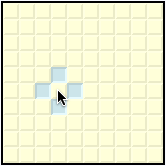
\includegraphics[width=.8\linewidth]{GameBoard}}
%	\caption{The Quinto game board. The user has just clicked the mouse as shown by the cursor.
%	\label{fig:gameBoard}}
%\end{wrapfigure}

\begin{figure}[ht]
	\vskip -\baselineskip
	\centerline{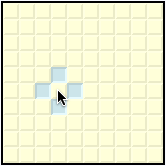
\includegraphics[width=.3\linewidth]{GameBoard}}
	\caption{Le plateau de jeu de Quinto. L'utilisateur vient de cliquer sur une case avec la souris comme le montre le curseur.
	\label{fig:gameBoard}}
\end{figure}

Pour vous montrer comment utiliser les outils de d\'eveloppement de \squeak, nous allons construire un jeu tr\`es simple nomm\'e \emph{Quinto}.  Le tableau de jeu est montr\'e dans \figref{gameBoard}; il consiste en un tableau rectangulaire de \emph{cellules} jaunes claires.  Lorsque l'on clique sur l'une de ces cellules avec la souris, les quatre qui l'entourent deviennent bleue. Cliquez de nouveau et elles repassent au jaune pale. Le but du jet est de passer au bleu autant de cellules que possible.

Le jeu de Quinto montr\'e dans \figref{gameBoard} est fait de deux types d'objets : le plateau de jeu lui-même et une centaine de cellule-objets individuels. Le code \squeak pour r\'ealiser ce jeu va contenir deux classes : une pour le jeu et une autre pour les cellules.
Nous allons voir maintenant comment d\'efinir ces deux classes en utilisant les outils de programmation de \squeak.

%=================================================================
\section{Créer une nouvelle catégorie de classe}

Nous avons déjà vu le \ind{navigateur de classes} (system browser) dans \charef{quick}, où nous avons appris à naviguer dans les classes et m\'ethodes et comment d\'efinir de nouvelles m\'ethodes.
Nous allons maintenant voir comment cr\'eer des cat\'egories syst\`emes et des classes.
\seeindex{system category}{category}
\seeindex{class category}{system category}
\index{category!creating}

\dothis{Ouvrir un navigateur de classes et cliquer avec le bouton jaune sur le panneau des cat\'egories.
S\'electionner \menu{add item \ldots}.}

\begin{figure}[htb]
\begin{minipage}[b]{0.48\textwidth}
\ifluluelse
	{\centerline {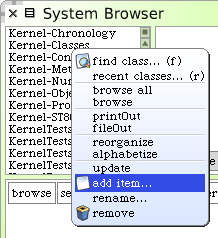
\includegraphics[width=0.9\textwidth]{AddCategory}}}
	{\centerline {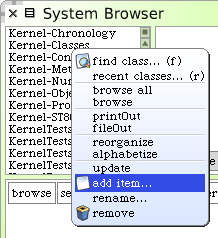
\includegraphics[scale=0.7]{AddCategory}}}
	\caption{Ajouter une cat\'egorie système.
	\label{fig:addCategory}}
\end{minipage}
\hfill
\begin{minipage}[b]{0.48\textwidth}
\ifluluelse
	{\centerline {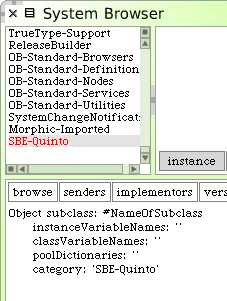
\includegraphics[width=0.9\textwidth]{ClassTemplate}}}
	{\centerline {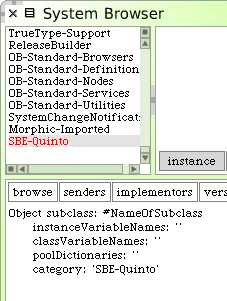
\includegraphics[scale=0.7]{ClassTemplate}}}
	\caption{Le modèle de création d'une classe.
	\label{fig:classTemplate}}
\end{minipage}
\end{figure}

Taper le nom de la nouvelle catégorie (nous allons utiliser \scat{SBE-Quinto}) dans la boîte de dialogue et cliquer sur \menu{accept} (ou appuyer juste la touche entrée); la nouvelle catégorie est créée et se positionne à la fin de la liste de catégories.
Si vous sélectionné une catégorie existante, alors la nouvelle catégorie sera positionnée juste après celle sélectionnée.

%=================================================================
\section{Définir la classe SBECell}

Pour l'instant, il n'y a aucune classe dans cette nouvelle catégorie. Néanmoins, la zone principale d'édition affiche un modèle afin de créer facilement une nouvelle classe (voir \figref{classTemplate}).

Ce modèle nous montre une expression \st qui envoie un message à la classe appellée \ct{Object}, lui demandant de créer une sous-classe appellée \ct{NameOfSubClass}.  La nouvelle classe n'a pas de variables et devrait appartenir à la catégorie \scat{SBE-Quinto}.

Nous modifions simplement le modèle afin de créer la classe que nous souhaitons.

\dothis{Modifier le modèle de création d'une classe comme suit :}
\begin{itemize}
  \item Remplacer \clsind{Object} par \clsind{SimpleSwitchMorph}.
  \item Remplacer \ct{NameOfSubClass} par \clsind{SBECell}.
  \item Ajouter \ct{mouseAction} dans la liste de variables d'instances.
\end{itemize}
Le résultat doit ressembler à \tclsref{firstClassDef}.

\begin{classdef}[firstClassDef]{Définition de la classe \ct| SBECell|}
SimpleSwitchMorph subclass: #SBECell
   instanceVariableNames: 'mouseAction'
   classVariableNames: ''
   poolDictionaries: ''
   category: 'SBE-Quinto'
\end{classdef}
\index{system browser!defining a class}
\index{class!creation}
\index{Morphic}

Cette nouvelle définition consiste en une expression \st qui envoie un message à une classe existante \ct{SimpleSwitchMorph}, lui demandant de créer une sous-classe appellée \ct{SBECell}.
(En fait, comme \ct{SBECell} n'existe pas encore, nous passons comme argument le \emphind{symbole} \ct{#SBECell} qui  correspond au nom de la classe à créer.)
Nous indiquons également que les instances de cette nouvelle classe doivent avoir une variable d'instance \ct{mouseAction}, que nous utiliserons pour définir l'action que la cellule doit effectuer lorsque l'utilisateur clique dessus avec la souris.

\emph{À ce point, nous n'avons encore rien construit.}
Notez que le bord du panneau du modèle de la classe est passé en rouge (\figref{acceptClassDef}).
Cela signifie qu'il y a des \emph{modifications non sauvegardées}.
Pour effectivement envoyer ce message, vous devez faire \menu{accept}.

\begin{figure}[h!t]
\ifluluelse
	{\centerline {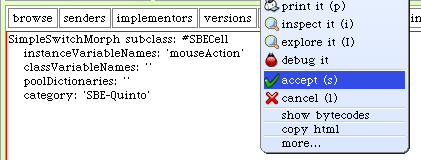
\includegraphics[width=\textwidth]{AcceptClassDef}}}
	{\centerline {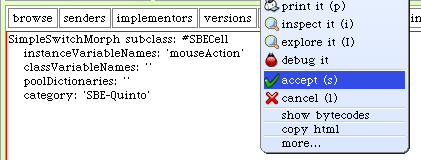
\includegraphics[scale=0.7]{AcceptClassDef}}}
\caption{Le modèle de création d'une classe.
\label{fig:acceptClassDef}}
\end{figure}

\dothis{Accepter la nouvelle définition de classe.}
Utiliser le clic jaune ou bien sélectionner \menu{accept} ou encore utiliser le raccourci clavier \short{s} (pour ``save'').
Ce message sera envoyé à \ct{SimpleSwitchMorph}, ce qui compilera la nouvelle classe.
\index{yellow button}
\index{keyboard shortcut!accept}

Une fois la définition de classe acceptée, la classe va être créée et apparaître dans le panneau des classes du navigateur (\figref{SBECell}).
Le panneau d'édition montre maintenant la définition de la classe et un petit panneau dessous vous invite à écrire quelques mots décrivant l'objectif de la classe. On appelle cela un \emph{commentaire de classe} et cela assez important d'en écrire un qui donnera aux autres développeurs une vision de haut niveau de votre classe.
Les Smalltalkiens accordent une grande valeur à la lisibilité de leur code et il est inusuel de trouver des commentaires détaillés dans leurs méthodes; la philosophie est plutôt d'avoir un code qui parle pour lui-même (si cela n'est pas le cas, vous devez le refactoriser, jusqu'à ce que le soit !). Un \subind{class}{commentaire} de classe ne nécessite pas une description détaillée de la classe, mais quelques mots la décrivant sont vital si les développeurs qui viennent après vous souhaitent passer un peu de temps sur votre classe.
\index{refactoring}

\dothis{Taper un commentaire de classe pour \ct{SBECell} et accepter le; vous aurez tout le loisir de l'améliorer par la suite.}

\begin{figure}[h!t]
\ifluluelse
	{\centerline {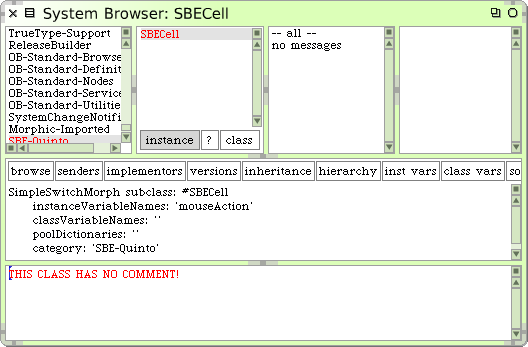
\includegraphics[width=\textwidth]{SBECell}}}
	{\centerline {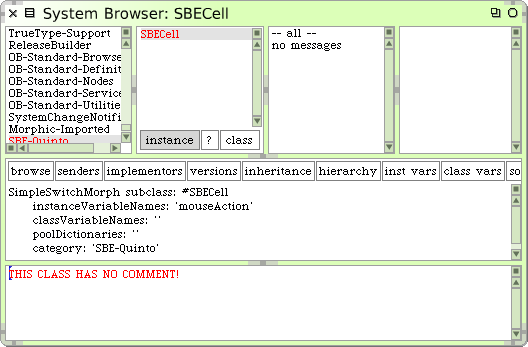
\includegraphics[scale=0.7]{SBECell}}}
\caption{La classe nouvellement créée \ct{SBECell}\label{fig:SBECell}}
\end{figure}

%=================================================================
\section{Ajouter des méthodes à la classe}

Ajoutons maintenant quelques méthodes à notre classe.

\dothis{Sélectionnez le protocole \prot{-{}-all-{}-} dans le panneau des contrôleurs.}
Vous voyez maintenant un modèle pour la création d'une méthode dans le panneau d'édition.
Sélectionnez le et remplacez le par le texte de \mthref{scbecellinitialize}.
\protindex{all}
\index{method!creation}
\index{system browser!defining a method}

\needlines{10}
\begin{numMethod}[scbecellinitialize]{Initialisation des instances de \ct{SBECell}}
initialize
   super initialize.
   self label: ''.
   self borderWidth: 2.
   bounds := 0@0 corner: 16@16.
   offColor := Color paleYellow.
   onColor := Color paleBlue darker.
   self useSquareCorners.
   self turnOff
\end{numMethod}
\index{initialization}

\noindent
Notez que les caractères \ct{''} de la ligne 3 sont deux quotes séparées avec rien entre les deux, et pas un guillemet ! \ct{''} représente la chaîne de caractères vide.

\dothis{Faire un \menu{accept} de cette définition de méthode.}

Que fait le code ci-dessus ?  Nous n'allons pas rentrer dans tous les détails maintenant (c'est l'objet du reste de ce livre !), mais nous allons vous en donner un bref aperçu. Prenons le ligne par ligne.

Notons que la méthode s'appelle \mthind{SBECell}{initialize}.
Ce nom dit bien ce qu'il veut dire !
Par convention, si une classe définit une méthode nommée \ct{initialize}, elle sera appellée dés que l'objet aura été créé.
Ainsi dés que nous évaluons \ct{SBECell new}, le message \ct{initialize} sera envoyé automatiquement à cet objet nouvellement créé.
Les méthodes d'initialisation sont utilisées pour définir l'état des objets, généralement pour donner une valeur à leurs variables d'instances; c'est exactement ce que nous faisons ici.
\seeindex{Object!initialization}{initialization}
\index{initialization}

La première chose que cette méthode fait (ligne 2) est d'exécuter la méthode \ct{initialize} de sa super-classe, \ct{SimpleSwitchMorph}.
L'idée est que tout état hérité sera initialisé correctement par la méthode \ct{initialize} de la super-classe.
C'est toujours une bonne idée d'initialiser l'état hérité en envoyant \ct{super initialize} avant de faire tout autre chose; nous ne savons pas exactement ce que la méthode \ct{initialize} de \ct{SimpleSwitchMorph} va faire, et nous ne nous en soucions pas, mais il est raisonnable de penser que cette méthode va initialiser quelques variables d'instance avec des valeurs par défaut, et qu'il faut mieux le faire sinon il y a le risque d'avoir un état incorrect.

Le reste de la méthode donne un état à cet objet.
Envoyer \ct{self label: ''} par exemple fixe le label de cet objet avec la chaîne de caractères vide.
\pvindex{self}

L'expression \ct{0@0 corner: 16@16} nécessite probablement plus d'explications.
\lct{0@0} représente un objet \clsind{Point} dont les coordonnées $x$ et $y$ ont été fixées à 0.
En fait, \ct{0@0} envoie le message \ct{@}% Yuck... the following should be \mthind{Number}{@} 
%%% THIS IS BROKEN -- don't do it! (on)
%\def\atsign{\textsf{@}}%
%{\makeatletter
%	\protected@write\@indexfile{}%
%    {\string\indexentry{\string\atsign|see{Number, \string\atsign}}{\thepage}}%
%	\protected@write\@indexfile{}%
%    {\string\indexentry{Number!\string\atsign|hyperpage}{\thepage}}%
%	\makeatother}
au nombre \ct{0} avec l'argument \ct{0}.
L'effet produit sera que le nombre \ct{0} va demander à la classe \ct{Point} de créer une nouvelle instance de coordonnées (0,0).
Puis, nous envoyons à ce nouveau point le message \ct{corner: 16@16}, ce qui cause la création d'un \clsind{Rectangle} de coins \ct{0@0} et \ct{16@16}.
Ce nouveau rectangle va être affecté à la variable \ct{bounds} héritée de la super-classe.

Notez que l'origine de l'écran \sq est en \emph{haut à gauche} et que les coordonnées en $y$ augmente \emph{vers le bas}.

Le reste de la méthode doit être compréhensible d'elle même.
Une partie de l'art d'écrire du bon code \st est de choisir les bons noms de méthodes de telle sorte que le code \st peut être lu comme du pidgin anglais.
Vous devriez être capable d'imaginer l'objet se parlant à lui-même et dire :  ``\ct{Utilise des bords carr\e's!}'', ``\ct{\'Eteinds les cellules!}''.

%=================================================================
\section{Inspecter un objet}

Vous pouvez tester l'effet du code que vous avez écrit en créant un nouvel objet \ct{SBECell} et en l'inspectant.

\dothis{Ouvrir un espace de travail. Tapez l'expression \ct{SBCell new} et choisir \menu{inspect it}.}

\begin{figure}[htbp]
   \centering
   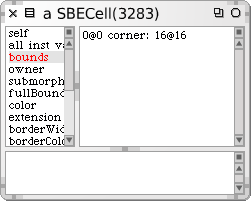
\includegraphics[scale=0.7]{SBECellInspector} 
   \caption{L'inspecteur utilisé pour examiner l'objet SBECell.\label{fig:SBECellInspector}}
\end{figure}

Le panneau gauche de l'\ind{inspecteur} montre une liste de variables d'instances; si vous en sélectionnez une (par exemple \mbox{\ct{bounds}),} la valeur de la \ind{variable d'instance} est affché dans le panneau droit. Vous pouvez également utiliser l'inspecteur pour changer la valeur d'une variable d'instance.

\dothis{Changer la valeur de \ct{bounds} à \ct{0@0 corner: 50@50} et  faire \menu{accept}.}

Le panneau en bas d'un inspecteur est un mini espace de travail (workspace). C'est très utile car dans cet espace de travail, la pseudo-variable \self est liée à l'objet inspecté.

\dothis{Tapez le texte \ct{self openInWorld} dans la zone du bas et choisir \menu{do it}.}
La cellule doit apparaître à l'angle haut à gauche de l'écran, en fait à l'endroit exact où sa sa variable \ct{bounds} dit qu'elle doit apparaître.
Faire un clic bleu sur la cellule afin de faire apparaître son \subind{Morphic}{halo} morphique.
Déplacer la cellule avec la poignée marron (à côte de celle en haut à droite) et redimensionner la avec la poignée jaune (en bas à droite).
Vérifier que les limites indiquées par l'inspecteur sont modifiées en conséquence.

\begin{figure}[htbp]
\centering
\ifluluelse
	{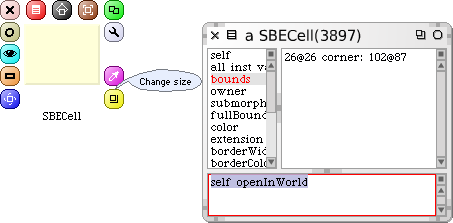
\includegraphics[width=\textwidth]{SBECellResize} }
	{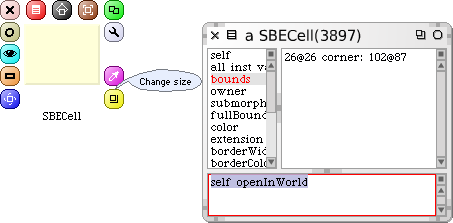
\includegraphics[scale=0.7]{SBECellResize} }
\caption{Redimensionner la cellule.\label{fig:cellresize}}
\end{figure}

\dothis{Détruire la cellule en cliquant sur le \ct{x} de la poignée mauve.}

%=================================================================
\section{Définir la classe SBEGame}

Crééons maintenant l'autre classe dont nous avons besoin dans le jeu, que nous appellerons \clsind{SBEGame}.

\dothis{Faire apparaître le modèle de définition de classe dans la fenêtre principale du navigateur.}
Pour cela re-sélectionner le nom de la catégorie de classe existante ou en affichant de nouveau la définition de \ct{SBECell} (en cliquant sur le bouton \button{instance}).
Éditer le code telle sorte qu'il peut être lu comme suit et faire \menu{accept}.

\needlines{6}
\begin{classdef}[sbegame]{Définition de la classe \ct{SBEGame}}
BorderedMorph subclass: #SBEGame
   instanceVariableNames: ''
   classVariableNames: ''
   poolDictionaries: ''
   category: 'SBE-Quinto'
\end{classdef}

Ici nous sous-classons \clsind{BorderedMorph}; \clsind{Morph} est la superclasse de toutes les formes graphiques de \squeak, et (suprise!) un \ct{BorderedMorph} est un \ct{Morph} avec un bord.  
Nous pouvons également insérer les noms des variables d'instances entre quote sur la seconde ligne, mais pour l'instant laissons cette liste vide.

Définissons maintenant une méthode \mthind{SBEGame}{initialize} pour \ct{SBEGame}.

\dothis{Tapez ce qui suit dans le navigateur comme une méthode de \ct{SBEGame} et faire ensuite \menu{accept} :}

\begin{numMethod}[sbegameinitialize]{Inialisation du jeu}
initialize
   | sampleCell width height n |
   super initialize.
   n := self cellsPerSide.
   sampleCell := SBECell new.
   width := sampleCell width.
   height := sampleCell height.
   self bounds: (5@5 extent: ((width*n) @(height*n)) + (2 * self borderWidth)).
   cells := Matrix new: n tabulate: [ :i :j | self newCellAt: i at: j ].
\end{numMethod}

%\sd{it would be nicer if we would not have to create an instance of SBECell for nothing}
%\on{yes}

\squeak va se plaindre qu'il ne connait pas la signification de certains termes.
\squeak vous indique qu'il ne connait pas le message \ct{cellsPerSide}, et suggère un certain nombre de propositions, dans le cas où il s'agirait d'une erreur de frappe.

\begin{figure}[htb]
\begin{minipage}{0.34\textwidth}
	\centering
	\ifluluelse
		{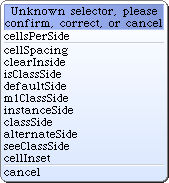
\includegraphics[width=\textwidth]{UnknownSelector}}
		{\includegraphics[scale=0.7]{UnknownSelector}}
	\caption{\squeak détecte un sélecteur inconnu.\label{fig:unknownSelector}}
\end{minipage}
\hfill
\begin{minipage}{0.64\textwidth}
	\centering
	\ifluluelse
		{\includegraphics[width=\textwidth]{DeclareInstanceVar}}
		{\includegraphics[scale=0.7]{DeclareInstanceVar}}
	\caption{Déclaration d'une nouvelle variable d'instance.\label{fig:declareInstance}}
\end{minipage}
\end{figure}

Mais \ct{cellsPerSide} n'est pas une erreur \,---\, c'est juste le nom d'une méthode que nous n'avons pas encore définie\,---\,que nous allons faire dans une minute ou deux.

\dothis{Sélectionner le premier élément du menu, afin de confirmer que nous parlons bien de \ct{cellsPerSide}.}

Puis, \squeak va se plaindre de ne pas connaître la signification \ct{cells}. Il vous offre plusieurs possibilités de le corriger.

\dothis{Choisir \menu{declare instance} parce que nous souhaitons que \ct{cells} soit une variable d'instance.}
Enfin, \squeak va se plaindre à propos du message \ct{newCellAt:at:} envoyé à la dernière ligne; ce n'est toujours pas une erreur, confirmez donc ce message également.
\index{on the fly variable definition}
\index{instance variable definition} 

Si vous regardez maintenant de nouveau la définition de classe (en cliquant sur le bouton \button{instance}), vous allez voir que la définition a été modifiée pour inclure la variable d'instance \ct{cells}.

Examinons plus précisemment cette méthode \ct{initialize}.
La ligne \ct{| sampleCell width height n |} déclare 4 variables temporaires. Elles sont appellées variables temporaires car leur portée et leur durée de vie sont limitées à cette méthode. Des variables temporaires avec des noms explicites sont utiles afin de rendre le code plus lisible. \st n'a pas de syntaxe spéciale pour distinguer les constantes et les variables et en fait ces 4 ``variables'' sont en fait des constantes. Les lignes 4 à 7 définissent les constantes.

Quelle taille doit faire notre plateau de jeu ? Big enough to hold some integral number of cells, and big enough to draw a border around them.
Quel est le bon nombre de cellules ? 5 ? 10 ? 100 ? Nous ne le savons pas pour l'instant et si nous savions, il y aurait des chances pour que nous changions par la suite d'idée par la suite. Nous déléguons donc la responsabilité de connaître ce nombre à une autre méthode, que nous appellons \ct{cellsPerSide}, et que nous écrirons dans une minute ou deux.
C'est parce que nous envoyons le message \ct{cellsPerSide} avant de définir une méthode avec ce nom que \squeak nous demande ``confirm, correct, or cancel'' lorsque nous acceptons le corps de la méthode \ct{initialize}.
Ne soyez pas inquiété par cela : c'est en fait une bonne pratique d'écrire en fonction d'autres méthodes qui ne sont pas encore définies.
Pourquoi ? En fait, ce n'est que quand nous avons commencé à écrire la méthode \ct{initialize} que nous nous sommes rendu compte que nous en avions besoin, et à ce point, nous lui avons donné un nom qui fait sens et nous avons poursuivi, sans nous interrompre.
 
La quatrième ligne utilise cette méthode : le code Smalltalk \ct{self cellsPerSide} envoie le message \ct{cellsPerSide} à \pvind{self}, i.e., à l'objet lui-même. La réponse, qui sera le nombre de cellules par côté du plateau de jeu est affecté à \ct{n}.

Les trois lignes suivantes créent un nouvel objet \ct{SBECell} et assigne sa largeur et sa hauteur aux variables temporaires appropriées.

%The eighth line sends the message \ct{bounds:} to \self.
%\ct{bounds:} is a method that we inherit from our superclass; it is used to define the space on the screen that this Morph will occupy.  
%The single colon (\ct{:}) at the end of the name says that \ct{bounds:} expects a single parameter, which should be a rectangle object.
La ligne 8 fixe la valeur de \ct{bounds} du nouvel objet.
Without worrying too much about the details just yet, just believe us that the expression in parentheses creates a square with its origin (\ie its top-left corner) at the point (5,5) and its bottom-right corner far enough away to allow space for the right number of cells.

The last line sets the \ct{SBEGame} object's instance variable \ct{cells} to a newly created \clsind{Matrix} with the right number of rows and columns.   We do this by sending the message \ct{new:tabulate:} to the \ct{Matrix} class (classes are objects too, so we can send them messages).  We know that \mthind{Matrix class}{new:tabulate:} takes two arguments because it has two colons (\ct{:}) in its name.   The arguments go right after the colons.
If you are used to languages that put all of the arguments together inside parentheses, this may seem weird at first.  Don't panic, it's only syntax!
It turns out to be a very good syntax because the name of the method can be used to explain the roles of the arguments.  For example, it is pretty clear that \ct{Matrix rows: 5 columns: 2} has 5 rows and 2 columns, and not 2 rows and 5 columns.
\cmindex{Matrix class}{rows:columns:}

\ct{Matrix new: n tabulate: [ :i :j | self newCellAt: i at: j ]} créée une nouvelle matrice de taille \ct{n}{$\times$}\ct{n} et initialise ses éléments. La valeur initiale de chaque élément dépend de ses coordonnées. L'élément \ct{(i,j)}\textsuperscript{th} sera initialisé avec le résultat de l'évaluation de \ct{self newCellAt: i at: j}.  

Voilà pour \ct{initialize}.  When you accept this message body, you might want to take the opportunity to pretty-up the formatting.  You don't have to do this by hand: from the the yellow-button menu select \menu{more \ldots \go prettyprint}, and the browser will do it for you\damien{this didn't do anything to me}.  You have to \menu{accept} again after you have \subind{method}{pretty-print}{}ed a method, or of course you can \subind{keyboard shortcut}{cancel} 
(\short{l}\,---\,that's a lower-case letter \emph{L}) if you don't like the result.
Alternatively, you can set up the browser to use the pretty-printer automatically whenever it shows you code: use the the right-most button in the button bar to adjust the view.
\seeindex{pretty-print}{method}

If you find yourself using \menu{more\,\ldots} a lot, it's useful to know that you can hold down the {\sc shift} key when you click to directly bring up the \menu{more \ldots} menu.

%=================================================================
\section{Organiser les méthodes en protocoles}

Avant de définir de nouvelles méthodes, attardons nous un peu sur le troisième panneau en haut du navigateur.
De la même façon que le premier panneau du navigateur nous permet de catégoriser les classes de telle sorte que nous ne soyons pas submergé par une liste de nom de classes trop longue dans le second panneau, le troisième panneau nous permet de catégoriser les méthodes de telle sorte que n'ayons pas pas une liste de méthodes trop longue dans le quatrième panneau.
Ces catégories de méthodes sont appellés ``protocoles''.
\index{protocol}

S'il y avait juste quelques méthodes par classes, ce niveau hiérarchique supplémentaire ne serait pas vraiment nécessaire.
C'est pour cela que le navigateur offre un protocole virtuel \prot{-{}-all-{}-}, qui vous ne serez pas surpris d'apprendre, contient toutes les méthodes de la classe.
\protindex{all}

\begin{figure}[htbp]
   \centering
   \includegraphics[scale=0.7]{Categorize} 
   \caption{Catégoriser toutes les méthodes non catégorisées.\label{fig:categorize}}
\end{figure}

Si vous avez suivi l'exemple jusqu'à présent, le troisième panneau doit contenir le protocole \protind{as yet unclassified}\footnote{NdT : non encore classifié}.

\dothis{Sélectionner avec le \ind{button jaune} l'élément du menu \menu{categorize all uncategorized} afin de régler ce problème et déplacer les méthodes \ct{initialize} vers un nouveau protocole appelé \protind{initialization}.}
Comment \squeak{} sait que c'est le bon protocole ? Well, in general \squeak{} can't know, but in this case there is also an \ct{initialize} method in a superclass, and \squeak assumes that our \ct{initialize} method should go in the same category as the one that it overrides.
\index{method!categorize}

You may find that \squeak has already put your \ct{initialize} method into the \protind{initialization} protocol.
If so, it's probably because you have loaded a package called \ct{AutomaticMethodCategorizer} into your image.

\paragraph{Une convention typographique.} Les Smalltalkiens utilisent fréquement la notation ``\verb|>>|'' afin d'identifier la classe à laquelle la méthode appartient, ainsi par exemple la méthode \ct{cellsPerSide} de la classe \ct{SBEGame} sera référencé comme \ct{SBEGame>>cellsPerSide}.
Afin d'indiquer que cela ne fait pas parti de la syntaxe de \st, nous utiliserons plutôt le symbole spécial \ct{>>>} de telle sorte que cette méthode apparaîtra dans le texte comme \ct{SBEGame>>>cellsPerSide}
\cmindex{Behavior}{>>}

From now on, when we show a method in this book, we will write the name of the method in this form.  Of course, when you actually type the code into the browser, you don't have to type the class name or the \ct{>>>}; instead, you just make sure that the appropriate class is selected in the class pane.  

Définissons maintenant les autres méthodes qui sont utilisées par la méthode \ct{SBEGame>>>initialize}. Les deux peuvent être mises dans le protocole \prot{initialization}.

\begin{method}[sbegamecellsperside]{Une méthode constante.}
SBEGame>>>cellsPerSide
   "The number of cells along each side of the game"
   ^ 10
\end{method}
\cmindex{SBEGame}{cellsPerSide}
\index{constant methods}

Cette méthode ne peut pas être plus simple : elle retourne la constante 10. Un avantage a représenter les constantes comme des méthodes est que si le programme évolue de telle sorte que la constante dépend d'autres propriétés, la méthode peut être modifiée pour calculer la valeur.

\needlines{10}
\begin{method}[newCellAt:at:]{Une méthode d'aide à l'initialisation.}
SBEGame>>>newCellAt: i at: j
   "Create a cell for position (i,j) and add it to my on-screen
   representation at the appropriate screen position.  Answer the new cell"
   | c origin |
   c := SBECell new.
   origin := self innerBounds origin.
   self addMorph: c.
   c position: ((i - 1) * c width) @ ((j - 1) * c height) + origin.
   c mouseAction: [self toggleNeighboursOfCellAt: i at: j ].
\end{method}
\cmindex{SBEGame}{newCellAt:at:}
%   ^ c      "omit this final line to create a bug"

\dothis{Ajouter les méthodes \ct{SBEGame>>>cellsPerSide} et \ct{SBEGame>>>newCellAt:at:}.}
Confirmer que les sélecteurs \ct{toggleNeighboursOfCellAt:at:} et \ct{mouseAction:} s'épellent correctement.

\Mthref{newCellAt:at:} answers a new SBECell, specialized to position \ct{(i, j)} in the \clsind{Matrix} of cells.
The last line defines the new cell's \ct{mouseAction} to be the \emph{block}
\mbox{\lct{[self toggleNeighboursOfCellAt: i at: j ]}.}
 In effect, this defines the callback behaviour to perform when the mouse is clicked.
The corresponding method also needs to be defined.

\begin{method}[toggleNeighboursOfCellAt:at:]{The callback method}
SBEGame>>>toggleNeighboursOfCellAt: i at: j
   (i > 1) ifTrue: [ (cells at: i - 1 at: j ) toggleState].
   (i < self cellsPerSide) ifTrue: [ (cells at: i + 1 at: j) toggleState].
   (j > 1) ifTrue: [ (cells at: i  at: j - 1) toggleState].
   (j < self cellsPerSide) ifTrue: [ (cells at: i at: j + 1) toggleState].
\end{method}
\cmindex{SBEGame}{toggleNeighboursOfCellAt:at:}

\Mthref{toggleNeighboursOfCellAt:at:} toggles the state of the four cells to the north, south, west and east of cell (\ct{i}, \ct{j}).  The only complication is that the board is finite, so we have to make sure that a neighboring cell exists before we toggle its state.

\dothis{Place this method in a new protocol called \prot{game logic}.\damien{this has to be explained. There were no explications before on how to create a new protocol.}}
To move the method, you can simply click on its name and drag it to the newly-created protocol (\figref{dragMethod}).

\begin{figure}[htbp]
   \centering
   \ifluluelse
		{\includegraphics[width=\textwidth]{DragMethod} }
		{\includegraphics[scale=0.7]{DragMethod} }
   \caption{Faire un glisser-déposer de la méthode dans un protocole.\label{fig:dragMethod}}
\end{figure}

To complete the Quinto game, we need to define two more methods in class \ct{SBECell} to handle mouse events.
\begin{method}[mouseAction:]{A typical setter method}
SBECell>>>mouseAction: aBlock
   ^ mouseAction := aBlock
\end{method}
\cmindex{SBECell}{mouseAction:}

\Mthref{mouseAction:} does nothing more than set the cell's \ct{mouseAction} variable to the argument, and then answers the new value.
Any method that \emph{changes} the value of an instance variable in this way is called a \emph{setter method}; a method that \emph{answers} the current value of an instance variable is called a \emph{getter method}.
\seeindex{setter method}{accessor}
\seeindex{getter method}{accessor}

If you are used to getters and setters in other programming languages, you might expect these methods to be called \ct{setmouseAction} and \ct{getmouseAction}.
The \st convention is different.
A getter always has the same name as the variable it gets, and a setter is named similarly, but with a trailing ``\ct{:}'', hence \ct{mouseAction} and \ct{mouseAction:}.

Collectively, setters and getters are called  \emphind{accessor} methods, and by convention they should be placed in the \protind{accessing} protocol.
In Smalltalk, \emph{all} instance variables are private to the object that owns them, so the only way for another object to read or write those variables in the Smalltalk language is through accessor methods like this one\footnote{In fact, the instance variables can be accessed in subclasses too.}.

\dothis{Go to the class \ct{SBECell}, define \ct{SBECell>>>mouseAction:} and put it in the \prot{accessing} protocol.}

Finally, we need to define a method \ct{mouseUp:}; this will be called automatically by the GUI framework if the mouse button is released while the mouse is over this cell on the screen.

\begin{method}[sbecellmouseup]{Un gestionnaire d'évènement.}
SBECell>>>mouseUp: anEvent
   mouseAction value
\end{method}
\cmindex{SBECell}{mouseUp:}

\dothis{Ajouter la méthode \ct{SBECell>>>mouseUp:} ensuite faire \menu{categorize all uncategorized}.}
\index{method!categorize}

What this method does is to send the message \ct{value} to the object stored in the instance variable \ct{mouseAction}. 
Recall that in \ct{SBEGame>>>newCellAt: i at: j} we assigned the following code fragment to \ct{mouseAction}:

\ct{[self toggleNeighboursOfCellAt: i at: j ]} 

\noindent
Sending the \ct{value} message causes this code fragment to be evaluated, and consequently the state of the cells will toggle.

%=================================================================
\section{Essayons notre code}

Voila, le jeu de Quinto est complet!

Si vous avez suivi toutes les étapes, vous devez pouvoir jouer au jeu qui consistent en 2 classes et 7 méthodes.

\dothis{Dans un espace de travail, tappez \ct{SBEGame new openInWorld} et faire \menu{do it}.}

The game will open, and you should be able to click on the cells and see how it works.

Well, so much for theory\ldots{}
When you click on a cell, a \emphind{notifier} window called the \clsind{PreDebugWindow}window appears with an error message!
As depicted in \figref{quintoError}, it says \ct{MessageNotUnderstood: SBEGame>>>toggleState}.

\begin{figure}[ht]
\ifluluelse
	{\centerline{\includegraphics[width=\textwidth]{Error}}}
	{\centerline{\includegraphics[scale=0.7]{Error}}}
\caption{Il y a une erreur dans notre jeu lorsqu'une cellule est sélectionnée !
\label{fig:quintoError}}
\end{figure}

\noindent
What happened? To find out, let's use one of Smalltalk's more powerful tools: the \ind{debugger}.

\dothis{Click on the \menu{debug} button in the notifer window.}
The debugger will appear.
In the upper part of the debugger window you can see the execution stack, showing all the active methods; selecting any one of them will show, in the middle pane, the Smalltalk code being executed in that method, with the part that triggered the error highlighted.

\dothis{Click on the line labelled
\ct{SBEGame>>>toggleNeighboursOfCellAt:at:} (near the top).}
The debugger will show you the \ind{execution context} within this method where the error occurred (\figref{debugToggle}).

\begin{figure}[ht]
\ifluluelse
	{\centerline {\includegraphics[width=\textwidth]{Debugger}}}
	{\centerline {\includegraphics[scale=0.7]{Debugger}}}
\caption{Le débogueur avec la méthode \ct{toggleNeighboursOfCell:at:} sélectionnée.
\label{fig:debugToggle}}
\end{figure}

At the bottom of the debugger are two small inspector windows.  On the left, you can inspect the object that is the receiver of the message that caused the selected method to execute, so you can look here to see the values of the instance variables.
On the right you can inspect an object that represents the currently executing method itself, so you can look here to see the values of the method's parameters and temporary variables.

Using the debugger, you can execute code step by step, inspect objects in parameters and local variables, evaluate code just as you can in a workspace, and, most surprisingly to those used to other debuggers, change the code while it is being debugged! Some Smalltalkers program in the debugger almost all the time, rather than in the browser.  The advantage of this is that you see the method that you are writing as it will be executed, with real parameters in the actual execution context.

In this case we can see in the first line of the top panel that the \ct{toggleState} message has been sent to an instance of \ct{SBEGame}, while it should clearly have been an instance of \lct{SBECell}.
The problem is most likely with the initialization of the \ct{cells} matrix.
Browsing the code of \cmind{SBEGame}{initialize} shows that \ct{cells} is filled with the return values of \ct{newCellAt:at:}, but when we look at that method, we see that there is no return statement there!
By default, a method returns \ct{self}, which in the case of \ct{newCellAt:at:} is indeed an instance of \ct{SBEGame}.
\index{method!returning self}

\dothis{Fermer la fen\^etre du d\'ebogueur.
Ajouter l'expression ``\ct{^ c}'' à la fin de la méthode \ct{SBEGame>>>newCellAt:at:} de telle sorte quelle retourne \ct{c}.
% It should now look as shown in \mthref{newCellAt:at:nobug}.}
(Voir \mthref{newCellAt:at:nobug}.)}

% \needlines{6}
\begin{method}[newCellAt:at:nobug]{Corriger l'erreur.}
SBEGame>>>newCellAt: i at: j
   "Create a cell for position (i,j) and add it to my on-screen
   representation at the appropriate screen position.  Answer the new cell"
   | c origin |
   c := SBECell new.
   origin := self innerBounds origin.
   self addMorph: c.
   c position: ((i - 1) * c width) @ ((j - 1) * c height) + origin.
   c mouseAction: [self toggleNeighboursOfCellAt: i at: j].
   ^ c
\end{method}
\cmindex{SBEGame}{newCellAt:at:}

\noindent
Recall from \charef{quick} that the construct to \ind{return} a \subind{method}{value} from a method in Smalltalk is \ct{^}, which you obtain by typing \verb|^|.
% \index{^@\verb|^|}
\index{^@{$\uparrow$}|see{return}}

Often, you can fix the code directly in the debugger window and click \menu{Proceed} to continue running the application.
In our case, because the bug was in the initialization of an object, rather than in the method that failed, the easiest thing to do is to close the debugger window, destroy the running instance of the game (with the \subind{Morphic}{halo}), and create a new one.

%Indeed, even in this case it would be possible to \menu{do} \ct{self initialize} and then \menu{Proceed} the \ct{toggleNeighboursOfCellAt:at:} method.
%\ab{St\'eph, did you try this?  It seems to me that it ought to work, but when I tried it, it messed up my image.}
% ON : It messed me up too!  Better not propose this.

\dothis{Exécuter : \ct{SBEGame new openInWorld} de nouveau.}
Le jeu doit maintenant se dérouler sans problèmes.

%\sd{It would be good to have a word about the debugger buttons into, step.... Or to have a separate chapter, we would use the material I wrote for my turtle book, please check it.}
%\on{I think that is too much for this chapter. It will come soon enough.}

%=================================================================
\section{Sauvegarder et partager le code Smalltalk}
\label{sec:Monticello}

Maintenant que nous avons un jeu de Quinto qui fonctionne, vous avez probablement envie de le sauvegarder quelque part de telle sorte à pouvoir le partager avec des amis. Bien sur, vous pouvez sauvegarder l'ensemble de votre image \squeak et montrer votre premier programme en l'exécutant, mais vos amis ont probablement leur propre code dans leurs images et ne veulent pas sans passer pour utiliser votre image.
Ce dont nous avons besoin est de pouvoir extraire le code source d'une image \squeak afin que d'autres développeurs puissent le charger dans leurs images.

The simplest way of doing this is by \emph{filing out} the code.  The yellow-button menu in the System Categories pane will give you the option to file out the whole of category \scat{SBE-Quinto}.
The resulting file is more or less human readable, but is really intended for computers, not humans.
You can email this file to your friends, and they can file it into their own \squeak images using the file list browser.
\seeindex{saving code}{categories}
\seeindex{category!filing out}{file, filing out}
\seeindex{class!filing out}{file, filing out}
\seeindex{method!filing out}{file, filing out}
\index{file!filing out}

\dothis{Yellow-click on the \scat{SBE-Quinto} category and \menu{fileOut} the contents.}
You should now find a file called ``SBE-Quinto.st'' in the same folder on disk where your image is saved.
Have a look at this file with a text editor.

\dothis{Open a fresh \squeak image and use the File List tool to \menu{file in} the SBE-Quinto.st fileout.
Verify that the game now works in the new image.}
\seeindex{category!filing in}{file, filing in}
\seeindex{class!filing in}{file, filing in}
\seeindex{method!filing in}{file, filing in}
\index{file!filing in}

\begin{figure}[ht]
\centerline {\includegraphics[width=\textwidth]{FileIn}}
\caption{Filing in \squeak source code.
\label{fig:filein}}
\end{figure}

\subsection{Les paquetages Monticello}
Although fileouts are a convenient way of making a snapshot of the code you have written, they are decidedly ``old school''.
Just as most open-source projects find it much more convenient to maintain their code in a repository using \ind{CVS}\footnote{\url{www.nongnu.org/cvs}} or \ind{Subversion}\footnote{\url{subversion.tigris.org}},
so \squeak programmers find it more convenient to manage their code using \ind{Monticello} packages. 
These packages are represented as files with names ending in \ct{.mcz}; they are actually zip-compressed bundles that contain the complete code of your \ind{package}.

Using the Monticello package browser, you can save packages to repositories on various types of server, including FTP and HTTP servers; you can also just write the packages to a repository in a local file system directory.
A copy of your package is also always cached on your local hard-disk in the \emph{package-cache} folder. 
Monticello lets you save multiple versions of your program, merge versions, go back to an old version, and browse the differences between versions. 
In fact, it supports the same sort of operations that you are used to if you share your work using CVS or Subversion.
\seeindex{package browser}{Monticello}

A good trick is to always develop in the same folder. This way you get a copy of all the code that you publish on squeaksource on your local machine. You can then backup and browse at will.

You can also send a \ct{.mcz} file by email. 
The recipient will have to place it in her \emph{package-cache} folder; she will then be able to use Monticello to browse and load it. 
%(It is also possible to load it using the file list, but there is a difference between loading a \ct{.mcz} file using a file list and using Monticello \sd{check}.)

\dothis{Open the Monticello browser by selecting \menu{World \go open\,\ldots \go Monticello browser}.}
In the right-hand pane of the browser (see \figref{monticello1}) is a list of Monticello repositories, which will include all of the repositories from which code has been loaded into the image that you are using.  
%In addition to SqueakSource servers, Monticello repositories can live in a variety of other places, the simplest being a directory on your local disk.

\begin{figure}[hbt]
\ifluluelse
	{\centerline {\includegraphics[width=\textwidth]{MonticelloBrowser}}}
	{\centerline {\includegraphics[scale=0.7]{MonticelloBrowser}}}
\caption{The Monticello browser.
\label{fig:monticello1}}
\end{figure}

At the top of the list in the Monticello browser is a repository in a local directory called the \emphind{package cache}, which caches copies of the packages that you have loaded or published over the network. This local cache is really handy because it lets you keep your own local history; it also allows you to work in places where you do not have internet access, or where access is slow enough that you do not want to save to a remote repository very frequently.


\subsection{Sauvegarder et charger du code avec Monticello.}
On the left-hand side of the Monticello browser is a list of packages that have a version loaded into the image; packages that have been modified since they were loaded are marked with an asterisk.  (These are sometimes referred to as \subind{package}{dirty} packages.)  If you select a package, the list of repositories is restricted to just those repositories that contain a copy of the selected package.
\seeindex{*}{package, dirty}
\seeindex{dirty package}{package, dirty}

What is a package?  For now, you can think of a package as a group of  class and method categories that share the same prefix.  Since we put all of the code for the Quinto game into the class category called \scat{SBE-Quinto}, we can refer to it as the \ct{SBE-Quinto} package.

\dothis{Ajouter le paquetage \ct{SBE-Quinto} à votre navigateur Monticello en utilisant le boutton \button{+Package}.}

\subsection{\ind{SqueakSource}: un \ind{SourceForge} pour \squeak.} 
Nous pensons que la meilleure façon de sauvegarder votre code et de le partager est de créer un compte sur un serveur SqueakSource\footnote{\url{http://www.squeaksource.com/}}.
SqueakSource est similaire à SourceForge\footnote{\url{http://sourceforge.net/}} : il s'agit d'un frontal web à un serveur Monticello HTTP qui vous permet de gérer vos projets.
%In addition, SqueakSource includes a wiki, remote code browsing, RSS feed, admin right and access right management,   
% A number of {SqueakSource servers} around the Internet provide Monticello repositories and other facilities for development projects, including as a Wiki for documentation, remote code browsing, an RSS feed for update notification, and automatic publishing on SqueakMap.
\lr{- Automatic publishing on SqueakMap does not work reliable anymore (the SqueakMap API changed several times), so better remove this part (p. 53)}
Il y a un serveur public SqueakSource à l'adresse \url{http://www.squeaksource.com/}, et une copie du code concernant ce livre est enregistré sur \url{http://www.squeaksource.com/SqueakByExample.html}. Vous pouvez consulter ce projet à l'aide d'un navigateur internet, mais il est beaucoup plus productif de le faire depuis \squeak, un outil ad-hoc appellé navigateur Monticello, qui vous permet de gérer vos paquetages.

\dothis{Ouvrir un navigateur web à l'adresse \url{http://www.squeaksource.com/}.
Ouvrir un compte et ensuite créer un projet (\ie ``register'').}
SqueakSource va vous montrer l'information que vous devez utiliser lorsque on ajoute un dépôt au moyen d'un navigateur Monticello.

Une fois que votre projet a été créé sur SqueakSource, vous devez indiquer au système \squeak comment l'utiliser.

\dothis{Avec le paquetage \ct{SBE-Quinto} sélectionné, cliquer le boutton \button{+Repository} dans le navigateur Monticello.}  Vous verrez une liste des différents type de dépôts disponible; pour ajouter un dépôt SqueakSource, sélectionner le menu \menu{HTTP}. You will be presented with a dialog in which you can provide the necessary information about the server.
You should copy the presented template to identify your SqueakSource project, paste it into Monticello and supply your initials and password:

\needlines{5}
\begin{code}{}
MCHttpRepository 
    location: 'http://www.squeaksource.com/!\emph{YourProject}!'
    user: '!\emph{yourInitials}!' 
    password: '!\emph{yourPassword}!'
\end{code}   

\noindent
If you provide empty initials and password strings, you can still load the project, but you will not be able to update it:

\needlines{5}
\begin{code}{}
MCHttpRepository 
    location: 'http://www.squeaksource.com/SqueakByExample'
    user: '' 
    password: ''
\end{code}   

%You can then load the code in your image by selecting the version you want. You can browse the code without loading it, using the \button{Browse} button.
Une fois que vous avez accepté ce modèle, un nouveau dépôt doit apparaître dans la partie droite du navigateur Monticello.

\begin{figure}[hbt]
\ifluluelse
	{\centerline {\includegraphics[width=\textwidth]{BrowseRepository}}}
	{\centerline {\includegraphics[scale=0.7]{BrowseRepository}}}
\caption{Parcourir un dépôt Monticello
\label{fig:monticello3}}
\end{figure}

\dothis{Cliquer sur le boutton \button{Save} pour faire une première sauvegarde de jeu Quinto sur SqueakSource.}

Pour charger un paquetage dans votre image, vous devez d'abord sélectionner une version particulière. Vous pouvez faire cela dans le navigateur de dépôt, que vous pouvez ouvrir avec le boutton \button{Open} ou le boutton jaune de la souris. Une fois que vous avez sélectionné une version, vous pouvez la charger dans votre image.

\dothis{Ouvrir le dépôt \ct{SBE-Quinto} que vous venez de sauvegarder.}

Monticello a beaucoup d'autres fonctionnalités qui seront discutées plus en détail au \charef{env}.
Vous pouvez également consulter la documentation en ligne pour Monticello à l'adresse \url{http://www.wiresong.ca/Monticello/}.

%=================================================================
\section{Résumé du chapitre}
Dans ce chapitre, nous avons vu comment créer des catégories, classes et méthodes. Nous avons vu comment utiliser le navigateur de classes (system browser), l'inspecteur, le débogueur et le gestionnaire Monticello.

\begin{itemize}
  \item Les catégories sont des groupes de classes qui ont à voir entre elles.
  \item Une nouvelle classe est créée en envoyant un message à sa super-classe.
  \item Les protocoles sont de groupes de méthodes qui ont à voir entre elles.
  \item Une nouvelle méthode est créée ou modifiée en éditant la définition dans le navigateur de classes et en \emph{acceptant} les modifications.
  \item L'inspecteur offre une manière simple et générale pour inspecter et interagir avec des objets arbitraires.
  \item Le navigateur de classes détecte l'utilisation de méthodes et de variables non déclarées et propose d'éventuelles corrections.
  \item La méthode \ct{initialize} est automatiquement éxecutée après la création d'un objet en \squeak. Vous pouvez y mettre tout code d'initialisation spécifique.
  \item Le débogueur procure un outil de haut-niveau pour inspecter et modifier l'état d'un programme en cours d'ex\'ecution.
  \item Vous pouvez partager le code source en le sauvegardant une catégorie sous forme d'un fichier.
  \item Une meilleure façon de partager le code est d'utiliser Monticello afin de gérer un dépôt externe, défini par exemple comme un projet SqueakSource.
\end{itemize}

%=================================================================
\ifx\wholebook\relax\else\end{document}\fi
%=================================================================
%=================================================================
%%% Local Variables:
%%% coding: utf-8
%%% mode: latex
%%% TeX-master: t
%%% TeX-PDF-mode: t
%%% ispell-local-dictionary: "english"
%%% End:
